\documentclass[10pt,letterpaper,twocolumn]{article}

\usepackage{amsmath}
\usepackage{amsfonts}
\usepackage{amssymb}
\usepackage{graphicx}
\usepackage[left=1cm,right=1cm,top=0.75cm,bottom=1.5cm]{geometry}
\usepackage{gensymb}
\usepackage{textgreek}
\usepackage{xcolor}
\usepackage[colorlinks]{hyperref}
	\hypersetup{
	colorlinks,
	linkcolor={red!50!black},
	citecolor={blue!60!black},
	urlcolor={blue!40!black}
	}
\usepackage{titlesec}
	\titleformat{\section}{\normalfont\large\scshape}{\thesection}{1em}{}
	\titleformat{\subsection}{\normalfont\normalsize\bfseries}{\thesubsection}{1em}{}
	\titleformat{\subsubsection}[runin]{\normalfont\normalsize\itshape}{\thesubsubsection}{1em}{}
	\titlespacing*{\section}{0pt}{5pt}{5pt}
	\titlespacing*{\subsection}{0pt}{5pt}{5pt}
	\titlespacing*{\subsubsection}{0pt}{5pt}{5pt}
\usepackage{savetrees}
\usepackage[font=footnotesize,labelfont=bf]{caption}
\usepackage[font=footnotesize,labelfont=bf]{subcaption}
\usepackage{courier}
\usepackage{listings}
	\lstset{
		language=R,
		basicstyle=\scriptsize\ttfamily,
		commentstyle=\ttfamily\color{gray},
		numbers=left,
		numberstyle=\ttfamily\color{gray}\footnotesize,
		stepnumber=1,
		numbersep=5pt,
		backgroundcolor=\color{white},
		showspaces=false,
		showstringspaces=false,
		showtabs=false,
		frame=single,
		tabsize=2,
		captionpos=b,
		breaklines=true,
		breakatwhitespace=false,
		title=\lstname,   
		commentstyle=\color{olive},
		keywordstyle=\color{blue},
		stringstyle=\color{purple},
		aboveskip=-10pt,
		belowskip=-10pt
	}
\usepackage[maxfloats=500]{morefloats}
\usepackage{textgreek}
\usepackage[capitalize]{cleveref}

\renewcommand\labelenumi{\textbf{(\theenumi)}}
\renewcommand{\thesubsection}{\thesection.\Alph{subsection}}
\usepackage{nth}
\setlength{\textfloatsep}{2pt plus 1.0pt minus 2.0pt}
\setlength{\floatsep}{2pt plus 2.0pt minus 2.0pt}
\setlength{\abovecaptionskip}{2pt plus 1.0pt minus 2.0pt}
\maxdeadcycles2000

\begin{document}

\begin{titlepage}
	\centering
	{\scshape\LARGE Quarterly Report\par}
	\vspace{1cm}
	{\scshape\Large Non-target Pesticide Effects Study\par}
	\vspace{1.5cm}
	{\huge\bfseries Summary of 2015 sample data\par}
	\vspace{2cm}
	{\Large\itshape {\href{mailto:majanse1@asu.edu}{Andrew Jansen}}\par}
	\vfill
	supervised by\par
	Dr.~Sangmi \textsc{Lee}\\
	Dr.~Nico \textsc{Franz}

	\vfill

% Bottom of the page
	{\large \today\par}
\end{titlepage}

\section{Exploration of sample mass - family count}\label{sec:mass-vs-count}
Initial statistical exploration of the relationship between sample mass and family level diversity was undertaken using simple linear regression for each block, site, sample date, and method, by insect order.
Assessment of this relationship is needed to evaluate the suitability of sample mass and family count as measures of insect abundance and diversity, respectively, and to characterize the degree to which these signals either support or contradict each other in quantifying non-target pesticide effects.
In summary, there appears to be a fixed effect of sample mass on family count, with random effects from each of the aforementioned factors.
However, the family count and mass data are not normally distributed (see \cref{sec:blocks,sec:bulk}), indicating the need for a general linear mixed model using either a Poisson or negative binomial distribution to make more robust inferences (see \cref{sec:glmm}).

In this section, all of the individual regressions, residual distributions, and normal probability plots are shown along with summary and test statistics for each regression.
Residual distribution and normal probability were only conducted where the insect order was present in samples from all three sampling methods.

%MALAISE TRAPS
\begin{figure}[h]
	\centering
	\begin{subfigure}[b]{0.15\textwidth}
		\caption{Mass vs. families}
		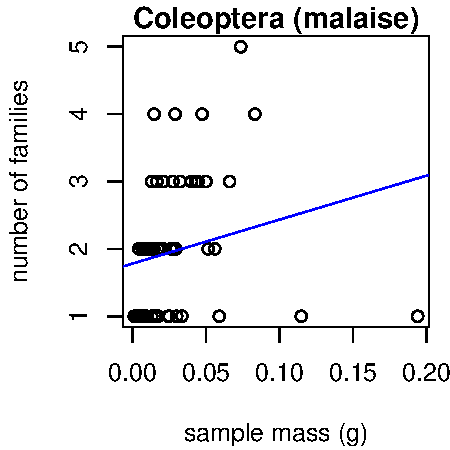
\includegraphics[width=\textwidth]{plots/mass-vs-count/scatter/2015_malaise_Coleoptera_mass-vs-count.pdf}
		\label{fig:malaise_coleoptera_scatter}
	\end{subfigure}
	~
	\begin{subfigure}[b]{0.15\textwidth}
		\caption{Residuals}
		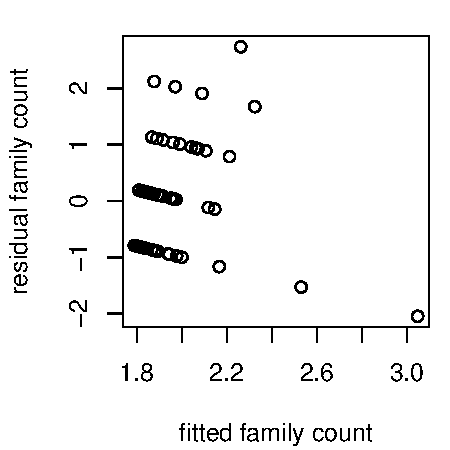
\includegraphics[width=\textwidth]{plots/mass-vs-count/residual/2015_malaise_Coleoptera_residual.pdf}
		\label{fig:malaise_coleoptera_resid}
	\end{subfigure}
	~
	\begin{subfigure}[b]{0.15\textwidth}
		\caption{Residual probability}
		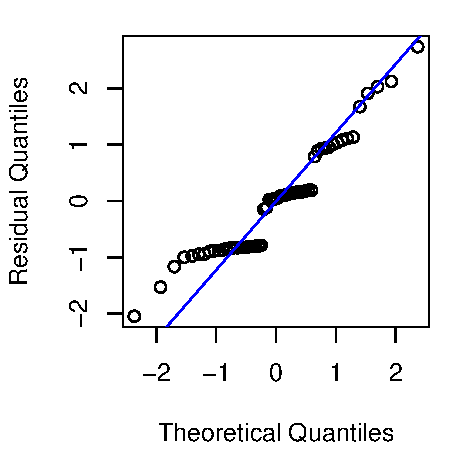
\includegraphics[width=\textwidth]{plots/mass-vs-count/qqplot/2015_malaise_Coleoptera_qqplot.pdf}
		\label{fig:malaise_coleoptera_qqplot}
	\end{subfigure}
	\caption{\textbf{(a)}~Scatter plot showing effect of sample mass on family count in malaise traps for order Coleoptera, with line of best fit (blue), \textbf{(b)}~scatter plot of fitted values and residuals, and \textbf{(c)}~normal probability plot of the residuals.}
	\label{fig:malaise_coleoptera}
	\smallskip
	\nointerlineskip
	\hrulefill
\end{figure}

\begin{figure}[h]
	\lstset{numbers=left}
	\lstset{xleftmargin=5mm,framexleftmargin=5mm}
	\begin{lstlisting}
malaise Coleoptera
Call:
lm(formula = temp.frame)

Residuals:
     Min       1Q   Median       3Q      Max 
-2.04754 -0.83021  0.04349  0.81422  2.73834 

Coefficients:
            Estimate Std. Error t value Pr(>|t|)    
(Intercept)   1.7813     0.1809   9.849 1.17e-13 ***
temp.mass     6.5272     4.2720   1.528    0.132    
---
Signif. codes:  0 '***' 0.001 '**' 0.01 '*' 0.05 '.' 0.1 ' ' 1

Residual standard error: 1.014 on 54 degrees of freedom
Multiple R-squared:  0.04144,	Adjusted R-squared:  0.02369 
F-statistic: 2.335 on 1 and 54 DF,  p-value: 0.1324
	\end{lstlisting}
	\caption{Verbatim R output of the results of linear regression of family count on sample mass in malaise traps for Coleoptera.}
	\label{fig:malaise_coleoptera_regression}
	\smallskip
	\nointerlineskip
	\hrulefill
\end{figure}

\begin{figure}[h]
	\centering
	\begin{subfigure}[b]{0.15\textwidth}
		\caption{Mass vs. families}
		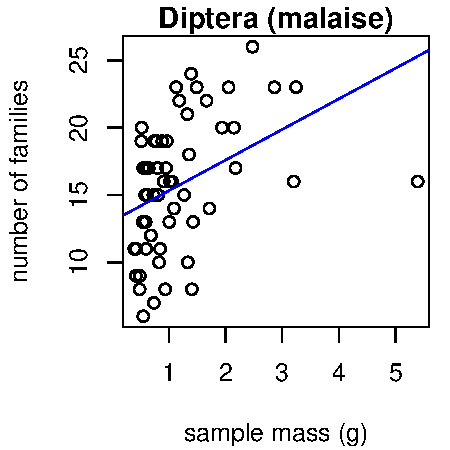
\includegraphics[width=\textwidth]{plots/mass-vs-count/scatter/2015_malaise_Diptera_mass-vs-count.pdf}
		\label{fig:malaise_diptera_scatter}
	\end{subfigure}
	~
	\begin{subfigure}[b]{0.15\textwidth}
		\caption{Residuals}
		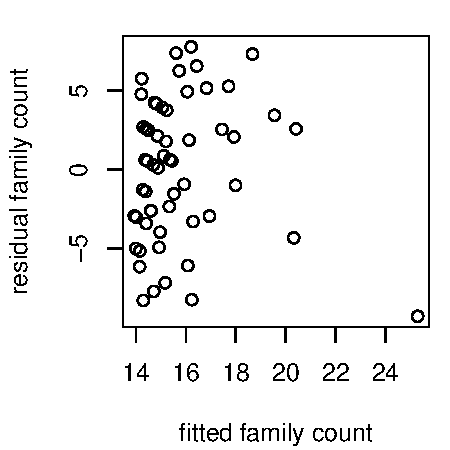
\includegraphics[width=\textwidth]{plots/mass-vs-count/residual/2015_malaise_Diptera_residual.pdf}
		\label{fig:malaise_diptera_resid}
	\end{subfigure}
	~
	\begin{subfigure}[b]{0.15\textwidth}
		\caption{Residual probability}
		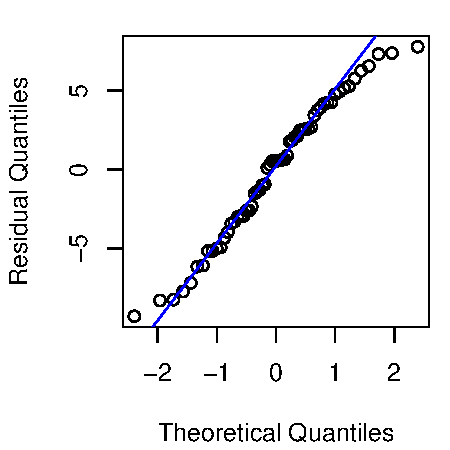
\includegraphics[width=\textwidth]{plots/mass-vs-count/qqplot/2015_malaise_Diptera_qqplot.pdf}
		\label{fig:malaise_diptera_qqplot}
	\end{subfigure}
	\caption{\textbf{(a)}~Scatter plot showing effect of sample mass on family count in malaise traps for order Diptera, with line of best fit (blue), \textbf{(b)}~scatter plot of fitted values and residuals, and \textbf{(c)}~normal probability plot of the residuals.}
	\label{fig:malaise_diptera}
	\smallskip
	\nointerlineskip
	\hrulefill
\end{figure}

\begin{figure}[h]
	\lstset{numbers=left}
	\lstset{xleftmargin=5mm,framexleftmargin=5mm}
	\begin{lstlisting}
malaise Diptera
Call:
lm(formula = temp.frame)

Residuals:
    Min      1Q  Median      3Q     Max 
-9.2933 -3.0763  0.5549  3.5269  7.7887 

Coefficients:
            Estimate Std. Error t value Pr(>|t|)    
(Intercept)  13.0480     0.9630  13.549  < 2e-16 ***
temp.mass     2.2715     0.6652   3.415  0.00117 ** 
---
Signif. codes:  0 '***' 0.001 '**' 0.01 '*' 0.05 '.' 0.1 ' ' 1

Residual standard error: 4.462 on 58 degrees of freedom
Multiple R-squared:  0.1674,	Adjusted R-squared:  0.153 
F-statistic: 11.66 on 1 and 58 DF,  p-value: 0.001171
	\end{lstlisting}
	\caption{Verbatim R output of the results of linear regression of family count on sample mass in malaise traps for Diptera.}
	\label{fig:malaise_diptera_regression}
	\smallskip
	\nointerlineskip
	\hrulefill
\end{figure}

\begin{figure}[h]
	\centering
	\begin{subfigure}[b]{0.15\textwidth}
		\caption{Mass vs. families}
		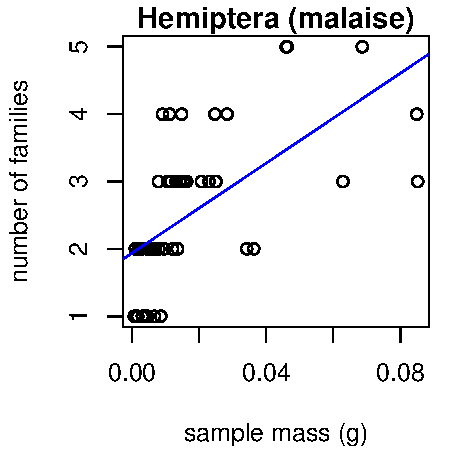
\includegraphics[width=\textwidth]{plots/mass-vs-count/scatter/2015_malaise_Hemiptera_mass-vs-count.pdf}
		\label{fig:malaise_hemiptera_scatter}
	\end{subfigure}
	~
	\begin{subfigure}[b]{0.15\textwidth}
		\caption{Residuals}
		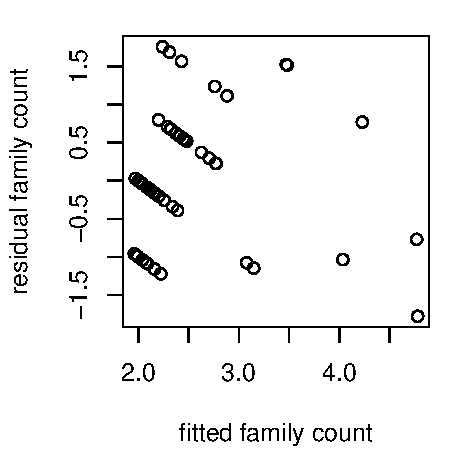
\includegraphics[width=\textwidth]{plots/mass-vs-count/residual/2015_malaise_Hemiptera_residual.pdf}
		\label{fig:malaise_hemiptera_resid}
	\end{subfigure}
	~
	\begin{subfigure}[b]{0.15\textwidth}
		\caption{Residual probability}
		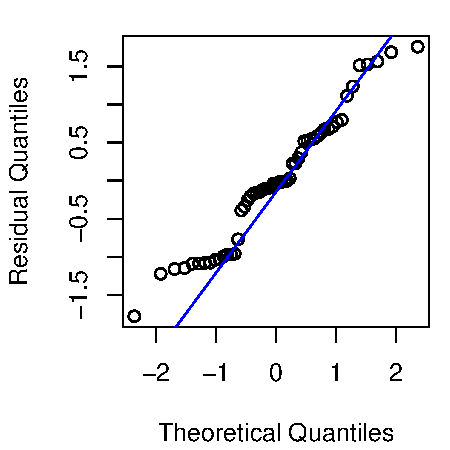
\includegraphics[width=\textwidth]{plots/mass-vs-count/qqplot/2015_malaise_Hemiptera_qqplot.pdf}
		\label{fig:malaise_hemiptera_qqplot}
	\end{subfigure}
	\caption{\textbf{(a)}~Scatter plot showing effect of sample mass on family count in malaise traps for order Hemiptera, with line of best fit (blue), \textbf{(b)}~scatter plot of fitted values and residuals, and \textbf{(c)}~normal probability plot of the residuals.}
	\label{fig:malaise_hemiptera}
	\smallskip
	\nointerlineskip
	\hrulefill
\end{figure}

\begin{figure}[h]
	\lstset{numbers=left}
	\lstset{xleftmargin=5mm,framexleftmargin=5mm}
	\begin{lstlisting}
malaise Hemiptera
Call:
lm(formula = temp.frame)

Residuals:
     Min       1Q   Median       3Q      Max 
-1.77990 -0.86472 -0.03631  0.56984  1.76009 

Coefficients:
            Estimate Std. Error t value Pr(>|t|)
(Intercept)   1.9362     0.1526  12.692  < 2e-16 ***
temp.mass    33.3770     5.9045   5.653 6.42e-07 ***
---
Signif. codes:  0 '***' 0.001 '**' 0.01 '*' 0.05 '.' 0.1 ' ' 1

Residual standard error: 0.8662 on 53 degrees of freedom
Multiple R-squared:  0.3761,	Adjusted R-squared:  0.3644 
F-statistic: 31.95 on 1 and 53 DF,  p-value: 6.424e-07
	\end{lstlisting}
	\caption{Verbatim R output of the results of linear regression of family count on sample mass in malaise traps for Hemiptera.}
	\label{fig:malaise_hemiptera_regression}
	\smallskip
	\nointerlineskip
	\hrulefill
\end{figure}

\begin{figure}[h]
	\centering
	\begin{subfigure}[b]{0.15\textwidth}
		\caption{Mass vs. families}
		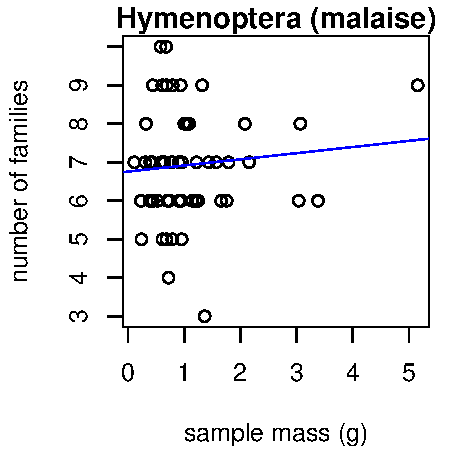
\includegraphics[width=\textwidth]{plots/mass-vs-count/scatter/2015_malaise_Hymenoptera_mass-vs-count.pdf}
		\label{fig:malaise_hymenoptera_scatter}
	\end{subfigure}
	~
	\begin{subfigure}[b]{0.15\textwidth}
		\caption{Residuals}
		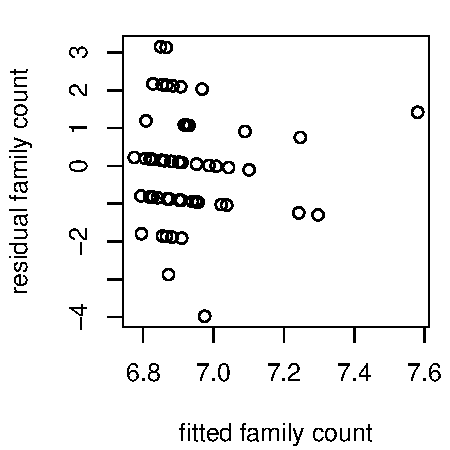
\includegraphics[width=\textwidth]{plots/mass-vs-count/residual/2015_malaise_Hymenoptera_residual.pdf}
		\label{fig:malaise_hymenoptera_resid}
	\end{subfigure}
	~
	\begin{subfigure}[b]{0.15\textwidth}
		\caption{Residual probability}
		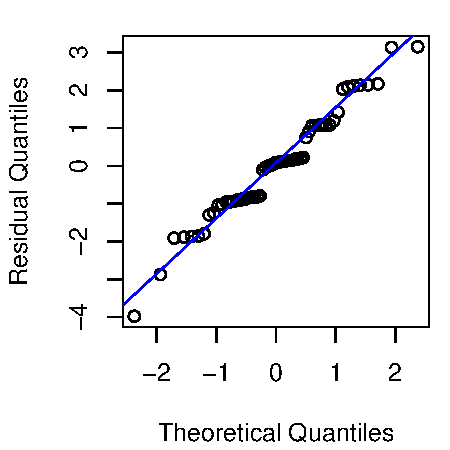
\includegraphics[width=\textwidth]{plots/mass-vs-count/qqplot/2015_malaise_Hymenoptera_qqplot.pdf}
		\label{fig:malaise_hymenoptera_qqplot}
	\end{subfigure}
	\caption{\textbf{(a)}~Scatter plot showing effect of sample mass on family count in malaise traps for order Hymenoptera, with line of best fit (blue), \textbf{(b)}~scatter plot of fitted values and residuals, and \textbf{(c)}~normal probability plot of the residuals.}
	\label{fig:malaise_hymenoptera}
	\smallskip
	\nointerlineskip
	\hrulefill
\end{figure}

\begin{figure}[h]
	\lstset{numbers=left}
	\lstset{xleftmargin=5mm,framexleftmargin=5mm}
	\begin{lstlisting}
malaise Hymenoptera
Call:
lm(formula = temp.frame)

Residuals:
    Min      1Q  Median      3Q     Max 
-3.9748 -0.9086  0.0898  1.0705  3.1505 

Coefficients:
            Estimate Std. Error t value Pr(>|t|)    
(Intercept)   6.7574     0.3053  22.131   <2e-16 ***
temp.mass     0.1595     0.2202   0.724    0.472    
---
Signif. codes:  0 '***' 0.001 '**' 0.01 '*' 0.05 '.' 0.1 ' ' 1

Residual standard error: 1.444 on 55 degrees of freedom
Multiple R-squared:  0.009444,	Adjusted R-squared:  -0.008566 
F-statistic: 0.5244 on 1 and 55 DF,  p-value: 0.4721
	\end{lstlisting}
	\caption{Verbatim R output of the results of linear regression of family count on sample mass in malaise traps for Hymenoptera.}
	\label{fig:malaise_hymenoptera_regression}
	\smallskip
	\nointerlineskip
	\hrulefill
\end{figure}

\begin{figure}[h]
	\centering
	\begin{subfigure}[b]{0.15\textwidth}
		\caption{Mass vs. families}
		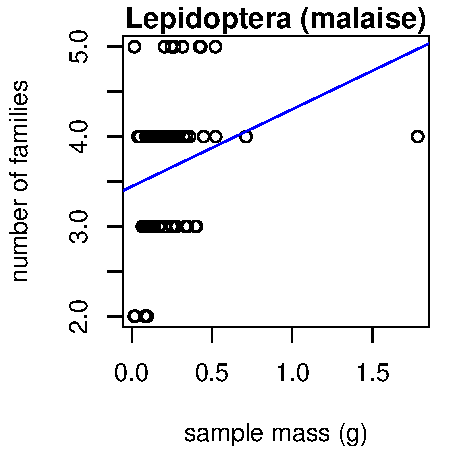
\includegraphics[width=\textwidth]{plots/mass-vs-count/scatter/2015_malaise_Lepidoptera_mass-vs-count.pdf}
		\label{fig:malaise_lepidoptera_scatter}
	\end{subfigure}
	~
	\begin{subfigure}[b]{0.15\textwidth}
		\caption{Residuals}
		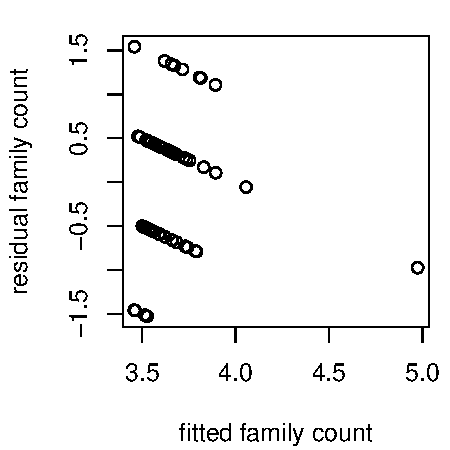
\includegraphics[width=\textwidth]{plots/mass-vs-count/residual/2015_malaise_Lepidoptera_residual.pdf}
		\label{fig:malaise_lepidoptera_resid}
	\end{subfigure}
	~
	\begin{subfigure}[b]{0.15\textwidth}
		\caption{Residual probability}
		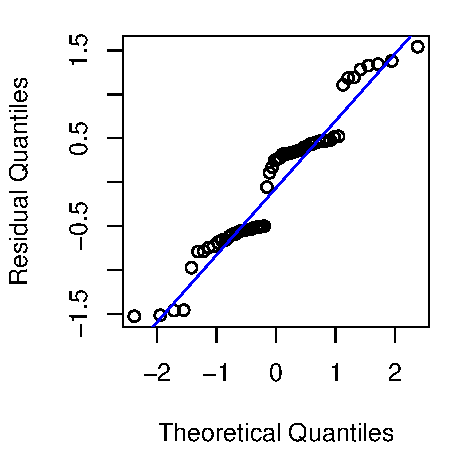
\includegraphics[width=\textwidth]{plots/mass-vs-count/qqplot/2015_malaise_Lepidoptera_qqplot.pdf}
		\label{fig:malaise_lepidoptera_qqplot}
	\end{subfigure}
	\caption{\textbf{(a)}~Scatter plot showing effect of sample mass on family count in malaise traps for order Lepidoptera, with line of best fit (blue), \textbf{(b)}~scatter plot of fitted values and residuals, and \textbf{(c)}~normal probability plot of the residuals.}
	\label{fig:malaise_lepidoptera}
	\smallskip
	\nointerlineskip
	\hrulefill
\end{figure}

\begin{figure}[h]
	\lstset{numbers=left}
	\lstset{xleftmargin=5mm,framexleftmargin=5mm}
	\begin{lstlisting}
malaise Lepidoptera
Call:
lm(formula = temp.frame)

Residuals:
    Min      1Q  Median      3Q     Max 
-1.5277 -0.5831  0.2536  0.4476  1.5408 

Coefficients:
            Estimate Std. Error t value Pr(>|t|)    
(Intercept)   3.4451     0.1444  23.864   <2e-16 ***
temp.mass     0.8582     0.4133   2.077   0.0424 *  
---
Signif. codes:  0 '***' 0.001 '**' 0.01 '*' 0.05 '.' 0.1 ' ' 1

Residual standard error: 0.7843 on 56 degrees of freedom
Multiple R-squared:  0.0715,	Adjusted R-squared:  0.05492 
F-statistic: 4.312 on 1 and 56 DF,  p-value: 0.04243
	\end{lstlisting}
	\caption{Verbatim R output of the results of linear regression of family count on sample mass in malaise traps for Lepidoptera.}
	\label{fig:malaise_lepidoptera_regression}
	\smallskip
	\nointerlineskip
	\hrulefill
\end{figure}

\begin{figure}[h]
	\centering
	\begin{subfigure}[b]{0.15\textwidth}
		\caption{Mass vs. families}
		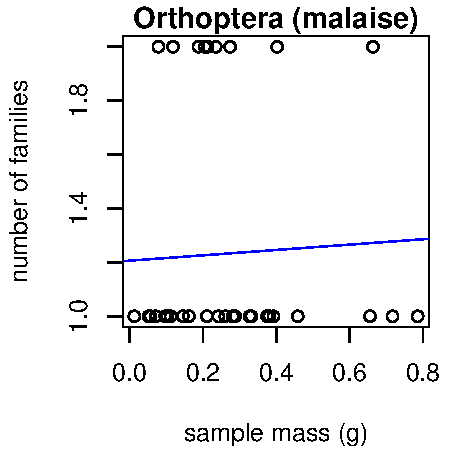
\includegraphics[width=\textwidth]{plots/mass-vs-count/scatter/2015_malaise_Orthoptera_mass-vs-count.pdf}
		\label{fig:malaise_orthoptera_scatter}
	\end{subfigure}
	~
	\begin{subfigure}[b]{0.15\textwidth}
		\caption{Residuals}
		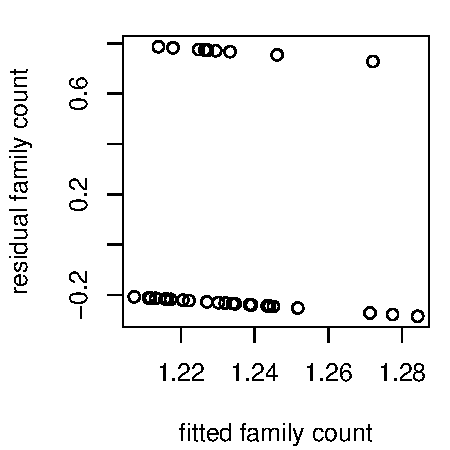
\includegraphics[width=\textwidth]{plots/mass-vs-count/residual/2015_malaise_Orthoptera_residual.pdf}
		\label{fig:malaise_orthoptera_resid}
	\end{subfigure}
	~
	\begin{subfigure}[b]{0.15\textwidth}
		\caption{Residual probability}
		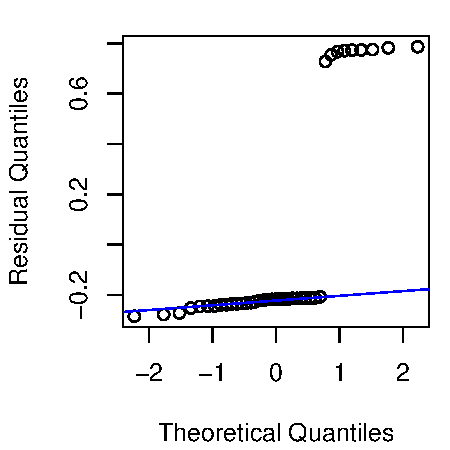
\includegraphics[width=\textwidth]{plots/mass-vs-count/qqplot/2015_malaise_Orthoptera_qqplot.pdf}
		\label{fig:malaise_orthoptera_qqplot}
	\end{subfigure}
	\caption{\textbf{(a)}~Scatter plot showing effect of sample mass on family count in malaise traps for order Orthoptera, with line of best fit (blue), \textbf{(b)}~scatter plot of fitted values and residuals, and \textbf{(c)}~normal probability plot of the residuals.}
	\label{fig:malaise_orthoptera}
	\smallskip
	\nointerlineskip
	\hrulefill
\end{figure}

\begin{figure}[h]
	\lstset{numbers=left}
	\lstset{xleftmargin=5mm,framexleftmargin=5mm}
	\begin{lstlisting}
malaise Orthoptera
Call:
lm(formula = temp.frame)

Residuals:
    Min      1Q  Median      3Q     Max 
-0.2843 -0.2346 -0.2163 -0.2093  0.7861 

Coefficients:
            Estimate Std. Error t value Pr(>|t|)    
(Intercept)  1.20611    0.11261  10.710 6.84e-13 ***
temp.mass    0.09944    0.35823   0.278    0.783    
---
Signif. codes:  0 '***' 0.001 '**' 0.01 '*' 0.05 '.' 0.1 ' ' 1

Residual standard error: 0.4321 on 37 degrees of freedom
Multiple R-squared:  0.002078,	Adjusted R-squared:  -0.02489 
F-statistic: 0.07706 on 1 and 37 DF,  p-value: 0.7829
	\end{lstlisting}
	\caption{Verbatim R output of the results of linear regression of family count on sample mass in malaise traps for Orthoptera.}
	\label{fig:malaise_orthoptera_regression}
	\smallskip
	\nointerlineskip
	\hrulefill
\end{figure}

\begin{figure}[h]
	\centering
	\begin{subfigure}[b]{0.15\textwidth}
		\caption{Mass vs. families}
		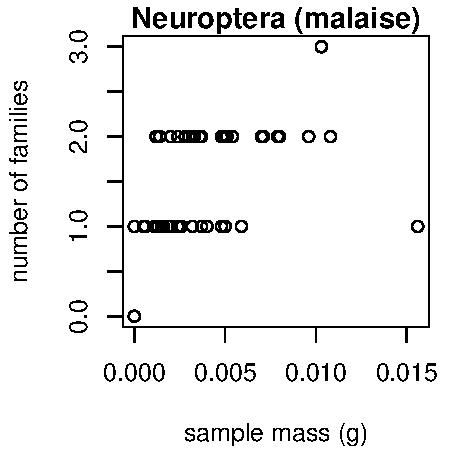
\includegraphics[width=\textwidth]{plots/mass-vs-count/scatter/2015_malaise_Neuroptera_mass-vs-count.pdf}
		\label{fig:malaise_neuroptera_scatter}
	\end{subfigure}
	\caption{Scatter plot showing effect of sample mass on family count in malaise traps: \textbf{(a)}~Neuroptera.}
	\label{fig:malaise_incomplete}
	\smallskip
	\nointerlineskip
	\hrulefill
\end{figure}

%PITFALL TRAPS

\begin{figure}[h]
	\centering
	\begin{subfigure}[b]{0.15\textwidth}
		\caption{Mass vs. families}
		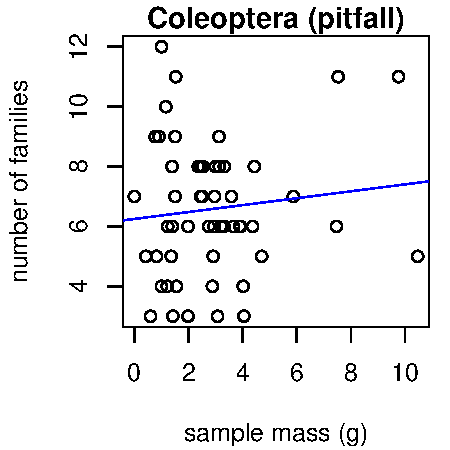
\includegraphics[width=\textwidth]{plots/mass-vs-count/scatter/2015_pitfall_Coleoptera_mass-vs-count.pdf}
		\label{fig:pitfall_coleoptera_scatter}
	\end{subfigure}
	~
	\begin{subfigure}[b]{0.15\textwidth}
		\caption{Residuals}
		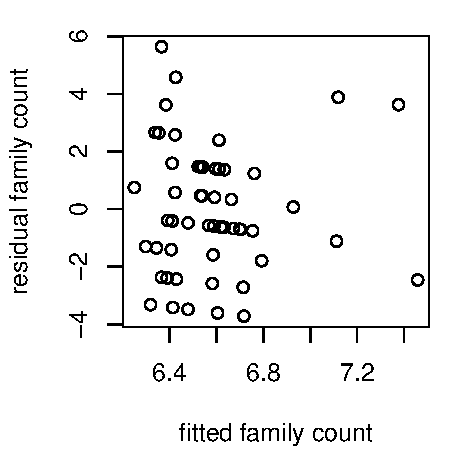
\includegraphics[width=\textwidth]{plots/mass-vs-count/residual/2015_pitfall_Coleoptera_residual.pdf}
		\label{fig:pitfall_coleoptera_resid}
	\end{subfigure}
	~
	\begin{subfigure}[b]{0.15\textwidth}
		\caption{Residual probability}
		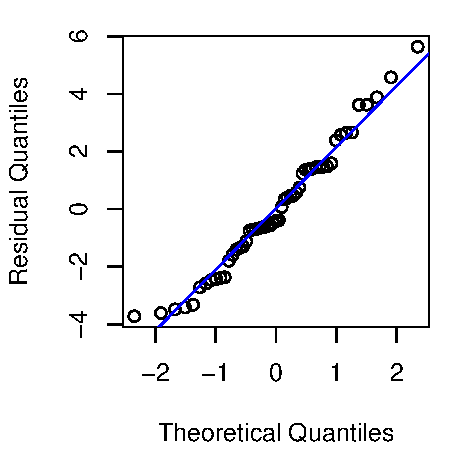
\includegraphics[width=\textwidth]{plots/mass-vs-count/qqplot/2015_pitfall_Coleoptera_qqplot.pdf}
		\label{fig:pitfall_coleoptera_qqplot}
	\end{subfigure}
	\caption{\textbf{(a)}~Scatter plot showing effect of sample mass on family count in pitfall traps for order Coleoptera, with line of best fit (blue), \textbf{(b)}~scatter plot of fitted values and residuals, and \textbf{(c)}~normal probability plot of the residuals.}
	\label{fig:pitfall_coleoptera}
	\smallskip
	\nointerlineskip
	\hrulefill
\end{figure}

\begin{figure}[h]
	\lstset{numbers=left}
	\lstset{xleftmargin=5mm,framexleftmargin=5mm}
	\begin{lstlisting}
pitfall Coleoptera
Call:
lm(formula = temp.frame)

Residuals:
    Min      1Q  Median      3Q     Max 
-3.7170 -1.4067 -0.4112  1.4579  5.6344 

Coefficients:
            Estimate Std. Error t value Pr(>|t|)    
(Intercept)   6.2494     0.5223  11.964   <2e-16 ***
temp.mass     0.1154     0.1452   0.795     0.43    
---
Signif. codes:  0 '***' 0.001 '**' 0.01 '*' 0.05 '.' 0.1 ' ' 1

Residual standard error: 2.239 on 51 degrees of freedom
Multiple R-squared:  0.01224,	Adjusted R-squared:  -0.007133 
F-statistic: 0.6317 on 1 and 51 DF,  p-value: 0.4304
	\end{lstlisting}
	\caption{Verbatim R output of the results of linear regression of family count on sample mass in pitfall traps for Coleoptera.}
	\label{fig:pitfall_coleoptera_regression}
	\smallskip
	\nointerlineskip
	\hrulefill
\end{figure}

\begin{figure}[h]
	\centering
	\begin{subfigure}[b]{0.15\textwidth}
		\caption{Mass vs. families}
		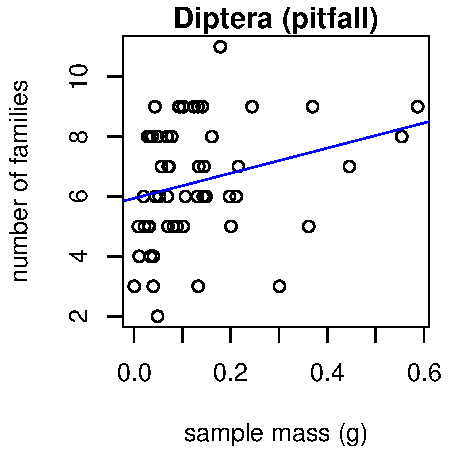
\includegraphics[width=\textwidth]{plots/mass-vs-count/scatter/2015_pitfall_Diptera_mass-vs-count.pdf}
		\label{fig:pitfall_diptera_scatter}
	\end{subfigure}
	~
	\begin{subfigure}[b]{0.15\textwidth}
		\caption{Residuals}
		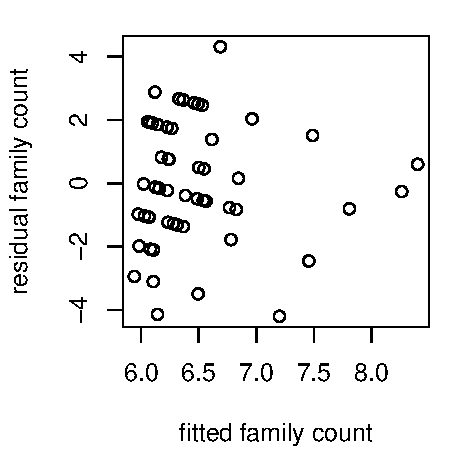
\includegraphics[width=\textwidth]{plots/mass-vs-count/residual/2015_pitfall_Diptera_residual.pdf}
		\label{fig:pitfall_diptera_resid}
	\end{subfigure}
	~
	\begin{subfigure}[b]{0.15\textwidth}
		\caption{Residual probability}
		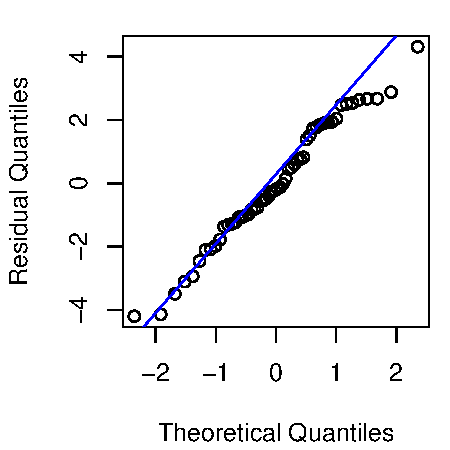
\includegraphics[width=\textwidth]{plots/mass-vs-count/qqplot/2015_pitfall_Diptera_qqplot.pdf}
		\label{fig:pitfall_diptera_qqplot}
	\end{subfigure}
	\caption{\textbf{(a)}~Scatter plot showing effect of sample mass on family count in pitfall traps for order Diptera, with line of best fit (blue), \textbf{(b)}~scatter plot of fitted values and residuals, and \textbf{(c)}~normal probability plot of the residuals.}
	\label{fig:pitfall_diptera}
	\smallskip
	\nointerlineskip
	\hrulefill
\end{figure}

\begin{figure}[h]
	\lstset{numbers=left}
	\lstset{xleftmargin=5mm,framexleftmargin=5mm}
	\begin{lstlisting}
pitfall Diptera
Call:
lm(formula = temp.frame)

Residuals:
   Min     1Q Median     3Q    Max 
-4.201 -1.193 -0.193  1.764  4.312 

Coefficients:
            Estimate Std. Error t value Pr(>|t|)    
(Intercept)   5.9393     0.3797  15.642   <2e-16 ***
temp.mass     4.1940     2.0891   2.008   0.0499 *  
---
Signif. codes:  0 '***' 0.001 '**' 0.01 '*' 0.05 '.' 0.1 ' ' 1

Residual standard error: 1.961 on 52 degrees of freedom
Multiple R-squared:  0.07193,	Adjusted R-squared:  0.05408 
F-statistic:  4.03 on 1 and 52 DF,  p-value: 0.0499
	\end{lstlisting}
	\caption{Verbatim R output of the results of linear regression of family count on sample mass in pitfall traps for Diptera.}
	\label{fig:pitfall_diptera_regression}
	\smallskip
	\nointerlineskip
	\hrulefill
\end{figure}

\begin{figure}[h]
	\centering
	\begin{subfigure}[b]{0.15\textwidth}
		\caption{Mass vs. families}
		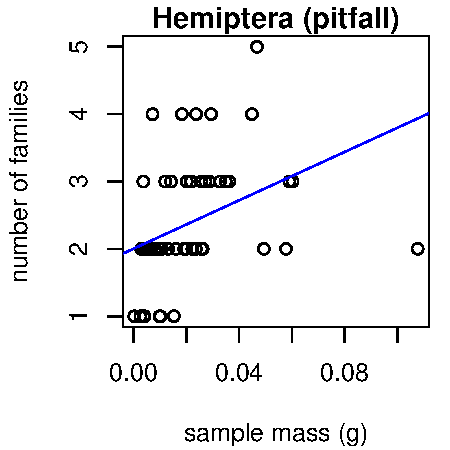
\includegraphics[width=\textwidth]{plots/mass-vs-count/scatter/2015_pitfall_Hemiptera_mass-vs-count.pdf}
		\label{fig:pitfall_hemiptera_scatter}
	\end{subfigure}
	~
	\begin{subfigure}[b]{0.15\textwidth}
		\caption{Residuals}
		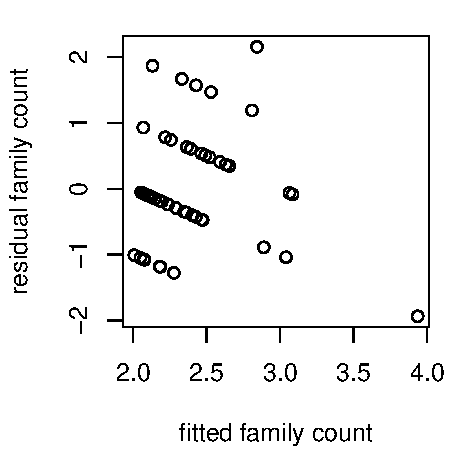
\includegraphics[width=\textwidth]{plots/mass-vs-count/residual/2015_pitfall_Hemiptera_residual.pdf}
		\label{fig:pitfall_hemiptera_resid}
	\end{subfigure}
	~
	\begin{subfigure}[b]{0.15\textwidth}
		\caption{Residual probability}
		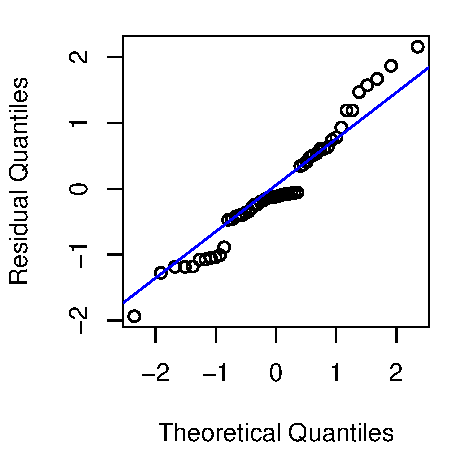
\includegraphics[width=\textwidth]{plots/mass-vs-count/qqplot/2015_pitfall_Hemiptera_qqplot.pdf}
		\label{fig:pitfall_hemiptera_qqplot}
	\end{subfigure}
	\caption{\textbf{(a)}~Scatter plot showing effect of sample mass on family count in pitfall traps for order Hemiptera, with line of best fit (blue), \textbf{(b)}~scatter plot of fitted values and residuals, and \textbf{(c)}~normal probability plot of the residuals.}
	\label{fig:pitfall_hemiptera}
	\smallskip
	\nointerlineskip
	\hrulefill
\end{figure}

\begin{figure}[h]
	\lstset{numbers=left}
	\lstset{xleftmargin=5mm,framexleftmargin=5mm}
	\begin{lstlisting}
pitfall Hemiptera
Call:
lm(formula = temp.frame)

Residuals:
    Min      1Q  Median      3Q     Max 
-1.9357 -0.4202 -0.1182  0.5295  2.1575 

Coefficients:
            Estimate Std. Error t value Pr(>|t|)    
(Intercept)   2.0024     0.1785  11.218 1.69e-15 ***
temp.mass    17.9510     6.1494   2.919  0.00518 ** 
---
Signif. codes:  0 '***' 0.001 '**' 0.01 '*' 0.05 '.' 0.1 ' ' 1

Residual standard error: 0.8797 on 52 degrees of freedom
Multiple R-squared:  0.1408,	Adjusted R-squared:  0.1243 
F-statistic: 8.521 on 1 and 52 DF,  p-value: 0.005177
	\end{lstlisting}
	\caption{Verbatim R output of the results of linear regression of family count on sample mass in pitfall traps for Hemiptera.}
	\label{fig:pitfall_hemiptera_regression}
	\smallskip
	\nointerlineskip
	\hrulefill
\end{figure}

\begin{figure}[h]
	\centering
	\begin{subfigure}[b]{0.15\textwidth}
		\caption{Mass vs. families}
		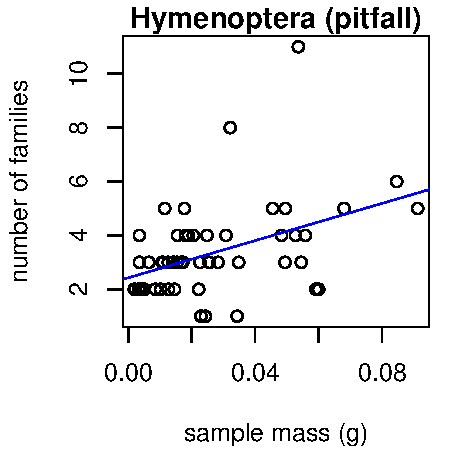
\includegraphics[width=\textwidth]{plots/mass-vs-count/scatter/2015_pitfall_Hymenoptera_mass-vs-count.pdf}
		\label{fig:pitfall_hymenoptera_scatter}
	\end{subfigure}
	~
	\begin{subfigure}[b]{0.15\textwidth}
		\caption{Residuals}
		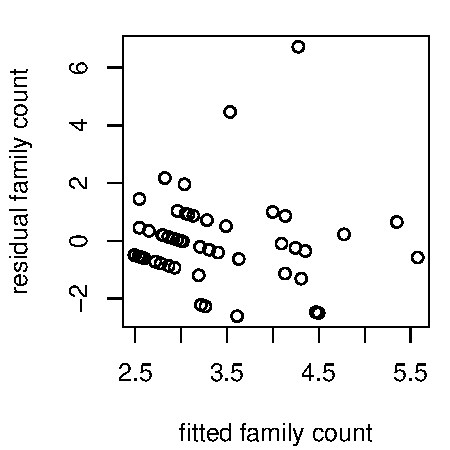
\includegraphics[width=\textwidth]{plots/mass-vs-count/residual/2015_pitfall_Hymenoptera_residual.pdf}
		\label{fig:pitfall_hymenoptera_resid}
	\end{subfigure}
	~
	\begin{subfigure}[b]{0.15\textwidth}
		\caption{Residual probability}
		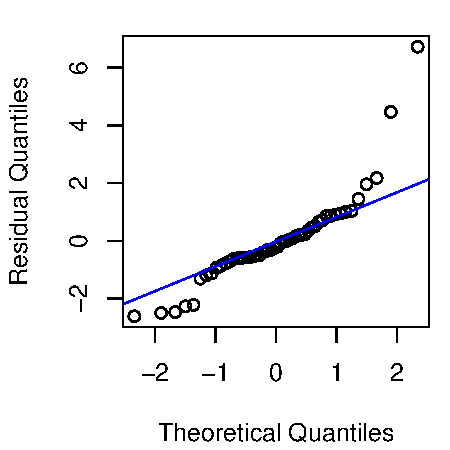
\includegraphics[width=\textwidth]{plots/mass-vs-count/qqplot/2015_pitfall_Hymenoptera_qqplot.pdf}
		\label{fig:pitfall_hymenoptera_qqplot}
	\end{subfigure}
	\caption{\textbf{(a)}~Scatter plot showing effect of sample mass on family count in pitfall traps for order Hymenoptera, with line of best fit (blue), \textbf{(b)}~scatter plot of fitted values and residuals, and \textbf{(c)}~normal probability plot of the residuals.}
	\label{fig:pitfall_hymenoptera}
	\smallskip
	\nointerlineskip
	\hrulefill
\end{figure}

\begin{figure}[h]
	\lstset{numbers=left}
	\lstset{xleftmargin=5mm,framexleftmargin=5mm}
	\begin{lstlisting}
pitfall Hymenoptera
Call:
lm(formula = temp.frame)

Residuals:
    Min      1Q  Median      3Q     Max 
-2.6107 -0.6090 -0.2264  0.5458  6.7230 

Coefficients:
            Estimate Std. Error t value Pr(>|t|)    
(Intercept)    2.427      0.344   7.053 4.96e-09 ***
temp.mass     34.523     10.017   3.446  0.00116 ** 
---
Signif. codes:  0 '***' 0.001 '**' 0.01 '*' 0.05 '.' 0.1 ' ' 1

Residual standard error: 1.566 on 50 degrees of freedom
Multiple R-squared:  0.1919,	Adjusted R-squared:  0.1758 
F-statistic: 11.88 on 1 and 50 DF,  p-value: 0.00116
	\end{lstlisting}
	\caption{Verbatim R output of the results of linear regression of family count on sample mass in pitfall traps for Hymenoptera.}
	\label{fig:pitfall_hymenoptera_regression}
	\smallskip
	\nointerlineskip
	\hrulefill
\end{figure}

\begin{figure}[h]
	\centering
	\begin{subfigure}[b]{0.15\textwidth}
		\caption{Mass vs. families}
		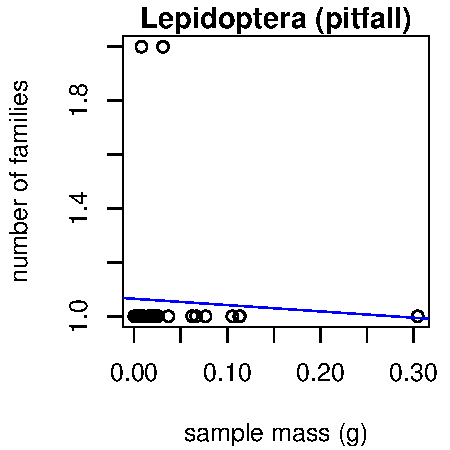
\includegraphics[width=\textwidth]{plots/mass-vs-count/scatter/2015_pitfall_Lepidoptera_mass-vs-count.pdf}
		\label{fig:pitfall_lepidoptera_scatter}
	\end{subfigure}
	~
	\begin{subfigure}[b]{0.15\textwidth}
		\caption{Residuals}
		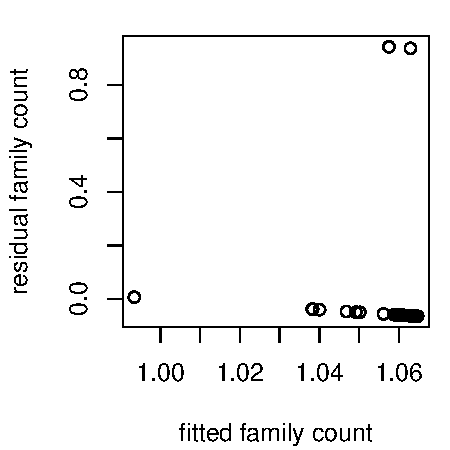
\includegraphics[width=\textwidth]{plots/mass-vs-count/residual/2015_pitfall_Lepidoptera_residual.pdf}
		\label{fig:pitfall_lepidoptera_resid}
	\end{subfigure}
	~
	\begin{subfigure}[b]{0.15\textwidth}
		\caption{Residual probability}
		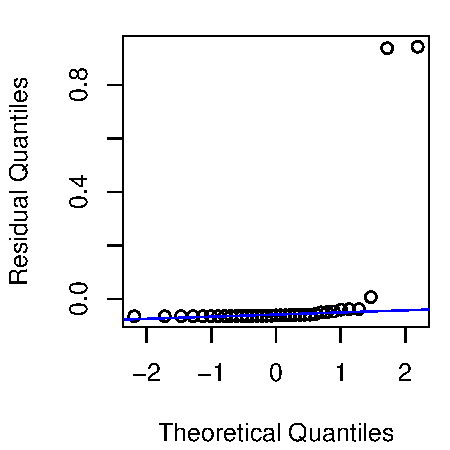
\includegraphics[width=\textwidth]{plots/mass-vs-count/qqplot/2015_pitfall_Lepidoptera_qqplot.pdf}
		\label{fig:pitfall_lepidoptera_qqplot}
	\end{subfigure}
	\caption{\textbf{(a)}~Scatter plot showing effect of sample mass on family count in pitfall traps for order Lepidoptera, with line of best fit (blue), \textbf{(b)}~scatter plot of fitted values and residuals, and \textbf{(c)}~normal probability plot of the residuals.}
	\label{fig:pitfall_lepidoptera}
	\smallskip
	\nointerlineskip
	\hrulefill
\end{figure}

\begin{figure}[h]
	\lstset{numbers=left}
	\lstset{xleftmargin=5mm,framexleftmargin=5mm}
	\begin{lstlisting}
pitfall Lepidoptera
Call:
lm(formula = temp.frame)

Residuals:
     Min       1Q   Median       3Q      Max 
-0.06474 -0.06390 -0.06120 -0.05319  0.94248 

Coefficients:
            Estimate Std. Error t value Pr(>|t|)    
(Intercept)  1.06481    0.04658  22.858   <2e-16 ***
temp.mass   -0.23442    0.71205  -0.329    0.744    
---
Signif. codes:  0 '***' 0.001 '**' 0.01 '*' 0.05 '.' 0.1 ' ' 1

Residual standard error: 0.2387 on 33 degrees of freedom
Multiple R-squared:  0.003274,	Adjusted R-squared:  -0.02693 
F-statistic: 0.1084 on 1 and 33 DF,  p-value: 0.7441
	\end{lstlisting}
	\caption{Verbatim R output of the results of linear regression of family count on sample mass in pitfall traps for Lepidoptera.}
	\label{fig:pitfall_lepidoptera_regression}
	\smallskip
	\nointerlineskip
	\hrulefill
\end{figure}

\begin{figure}[h]
	\centering
	\begin{subfigure}[b]{0.15\textwidth}
		\caption{Mass vs. families}
		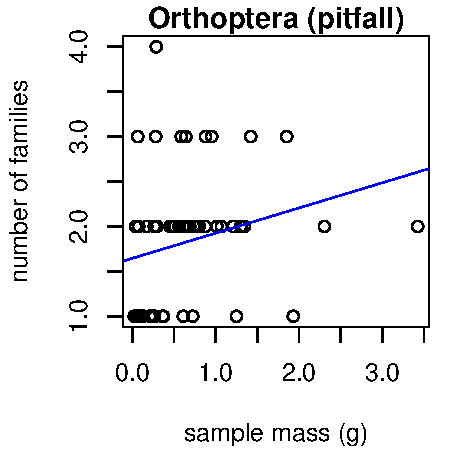
\includegraphics[width=\textwidth]{plots/mass-vs-count/scatter/2015_pitfall_Orthoptera_mass-vs-count.pdf}
		\label{fig:pitfall_orthoptera_scatter}
	\end{subfigure}
	~
	\begin{subfigure}[b]{0.15\textwidth}
		\caption{Residuals}
		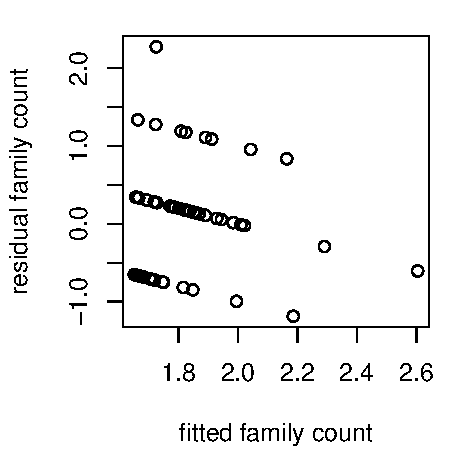
\includegraphics[width=\textwidth]{plots/mass-vs-count/residual/2015_pitfall_Orthoptera_residual.pdf}
		\label{fig:pitfall_orthoptera_resid}
	\end{subfigure}
	~
	\begin{subfigure}[b]{0.15\textwidth}
		\caption{Residual probability}
		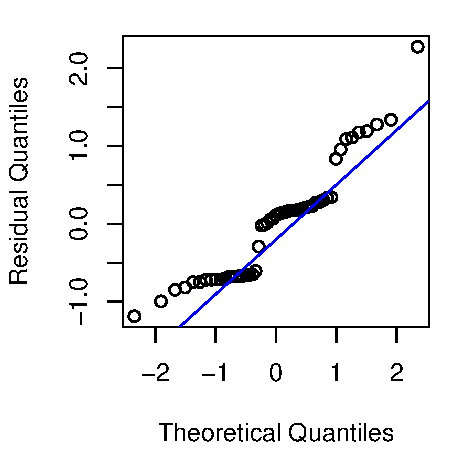
\includegraphics[width=\textwidth]{plots/mass-vs-count/qqplot/2015_pitfall_Orthoptera_qqplot.pdf}
		\label{fig:pitfall_orthoptera_qqplot}
	\end{subfigure}
	\caption{\textbf{(a)}~Scatter plot showing effect of sample mass on family count in pitfall traps for order Orthoptera, with line of best fit (blue), \textbf{(b)}~scatter plot of fitted values and residuals, and \textbf{(c)}~normal probability plot of the residuals.}
	\label{fig:pitfall_orthoptera}
	\smallskip
	\nointerlineskip
	\hrulefill
\end{figure}

\begin{figure}[h]
	\lstset{numbers=left}
	\lstset{xleftmargin=5mm,framexleftmargin=5mm}
	\begin{lstlisting}
pitfall Orthoptera
Call:
lm(formula = temp.frame)

Residuals:
    Min      1Q  Median      3Q     Max 
-1.1864 -0.6755  0.1094  0.2725  2.2746 

Coefficients:
            Estimate Std. Error t value Pr(>|t|)    
(Intercept)   1.6454     0.1454  11.317 1.61e-15 ***
temp.mass     0.2801     0.1579   1.773   0.0822 .  
---
Signif. codes:  0 '***' 0.001 '**' 0.01 '*' 0.05 '.' 0.1 ' ' 1

Residual standard error: 0.7378 on 51 degrees of freedom
Multiple R-squared:  0.05807,	Adjusted R-squared:  0.0396 
F-statistic: 3.144 on 1 and 51 DF,  p-value: 0.08218
	\end{lstlisting}
	\caption{Verbatim R output of the results of linear regression of family count on sample mass in pitfall traps for Orthoptera.}
	\label{fig:pitfall_orthoptera_regression}
	\smallskip
	\nointerlineskip
	\hrulefill
\end{figure}

\begin{figure}[h]
	\centering
	\begin{subfigure}[b]{0.15\textwidth}
		\caption{Mass vs. families}
		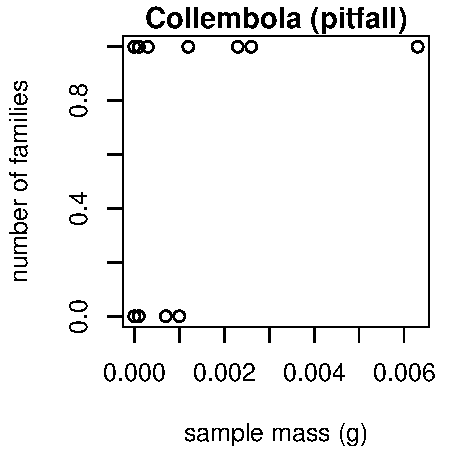
\includegraphics[width=\textwidth]{plots/mass-vs-count/scatter/2015_pitfall_Collembola_mass-vs-count.pdf}
		\label{fig:pitfall_collembola_scatter}
	\end{subfigure}
	~
	\begin{subfigure}[b]{0.15\textwidth}
		\caption{Mass vs. families}
		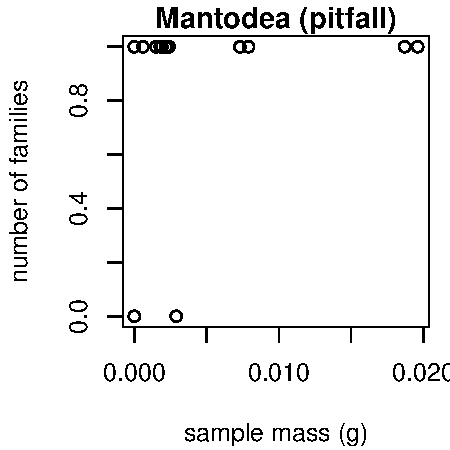
\includegraphics[width=\textwidth]{plots/mass-vs-count/scatter/2015_pitfall_Mantodea_mass-vs-count.pdf}
		\label{fig:pitfall_mantodea_scatter}
	\end{subfigure}
	~
	\begin{subfigure}[b]{0.15\textwidth}
		\caption{Mass vs. families}
		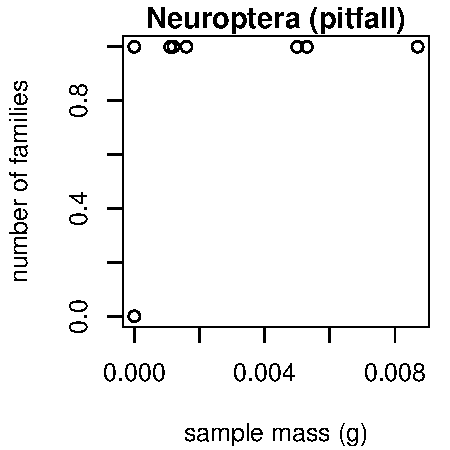
\includegraphics[width=\textwidth]{plots/mass-vs-count/scatter/2015_pitfall_Neuroptera_mass-vs-count.pdf}
		\label{fig:pitfall_neuroptera_scatter}
	\end{subfigure}
	~
	\begin{subfigure}[b]{0.15\textwidth}
		\caption{Mass vs. families}
		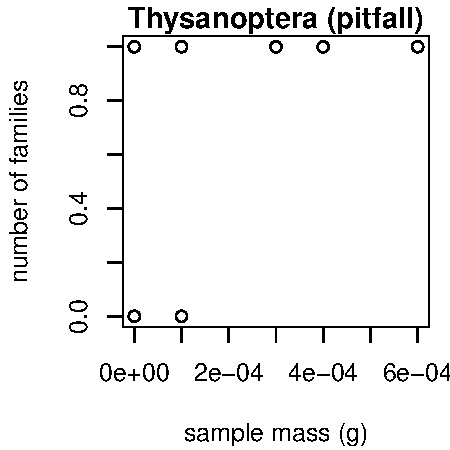
\includegraphics[width=\textwidth]{plots/mass-vs-count/scatter/2015_pitfall_Thysanoptera_mass-vs-count.pdf}
		\label{fig:pitfall_thysanoptera_scatter}
	\end{subfigure}
	\caption{Scatter plot showing effect of sample mass on family count in pitfall traps: \textbf{(a)}~Collembola, \textbf{(b)}~Mantodea, \textbf{(c)}~Neuroptera, \textbf{(d)}~Thysanoptera.}
	\label{fig:pitfall_incomplete}
	\smallskip
	\nointerlineskip
	\hrulefill
\end{figure}

%SWEEP NETTING

\begin{figure}[h]
	\centering
	\begin{subfigure}[b]{0.15\textwidth}
		\caption{Mass vs. families}
		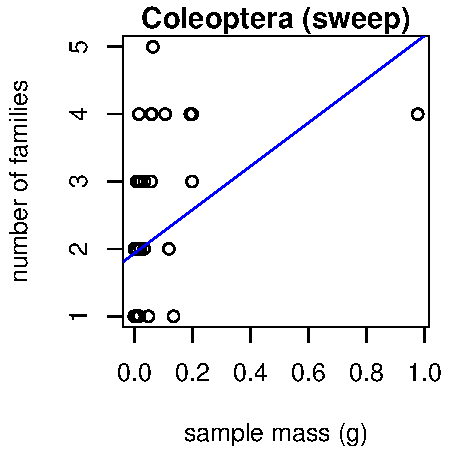
\includegraphics[width=\textwidth]{plots/mass-vs-count/scatter/2015_sweep_Coleoptera_mass-vs-count.pdf}
		\label{fig:sweep_coleoptera_scatter}
	\end{subfigure}
	~
	\begin{subfigure}[b]{0.15\textwidth}
		\caption{Residuals}
		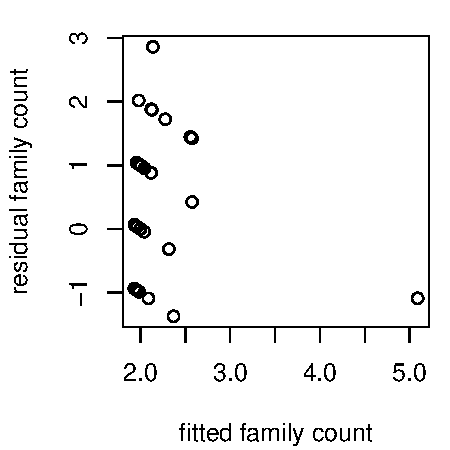
\includegraphics[width=\textwidth]{plots/mass-vs-count/residual/2015_sweep_Coleoptera_residual.pdf}
		\label{fig:sweep_coleoptera_resid}
	\end{subfigure}
	~
	\begin{subfigure}[b]{0.15\textwidth}
		\caption{Residual probability}
		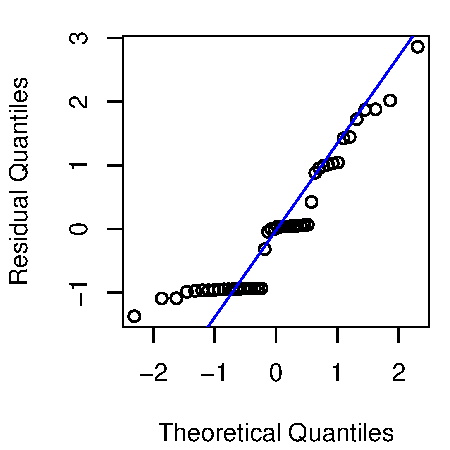
\includegraphics[width=\textwidth]{plots/mass-vs-count/qqplot/2015_sweep_Coleoptera_qqplot.pdf}
		\label{fig:sweep_coleoptera_qqplot}
	\end{subfigure}
	\caption{\textbf{(a)}~Scatter plot showing effect of sample mass on family count in sweep samples for order Coleoptera, with line of best fit (blue), \textbf{(b)}~scatter plot of fitted values and residuals, and \textbf{(c)}~normal probability plot of the residuals.}
	\label{fig:sweep_coleoptera}
	\smallskip
	\nointerlineskip
	\hrulefill
\end{figure}

\begin{figure}[h]
	\lstset{numbers=left}
	\lstset{xleftmargin=5mm,framexleftmargin=5mm}
	\begin{lstlisting}
sweep Coleoptera
Call:
lm(formula = temp.frame)

Residuals:
     Min       1Q   Median       3Q      Max 
-1.36994 -0.94297  0.01772  0.89865  2.85965 

Coefficients:
            Estimate Std. Error t value Pr(>|t|)    
(Intercept)   1.9324     0.1636  11.815 1.56e-15 ***
temp.mass     3.2291     1.0619   3.041  0.00389 ** 
---
Signif. codes:  0 '***' 0.001 '**' 0.01 '*' 0.05 '.' 0.1 ' ' 1

Residual standard error: 1.063 on 46 degrees of freedom
Multiple R-squared:  0.1674,	Adjusted R-squared:  0.1493 
F-statistic: 9.247 on 1 and 46 DF,  p-value: 0.003887
	\end{lstlisting}
	\caption{Verbatim R output of the results of linear regression of family count on sample mass in sweep samples for Coleoptera.}
	\label{fig:sweep_coleoptera_regression}
	\smallskip
	\nointerlineskip
	\hrulefill
\end{figure}

\begin{figure}[h]
	\centering
	\begin{subfigure}[b]{0.15\textwidth}
		\caption{Mass vs. families}
		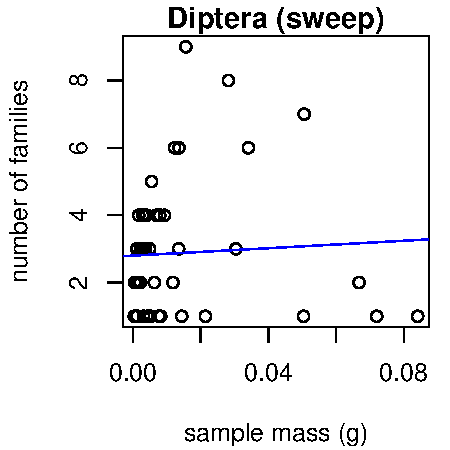
\includegraphics[width=\textwidth]{plots/mass-vs-count/scatter/2015_sweep_Diptera_mass-vs-count.pdf}
		\label{fig:sweep_diptera_scatter}
	\end{subfigure}
	~
	\begin{subfigure}[b]{0.15\textwidth}
		\caption{Residuals}
		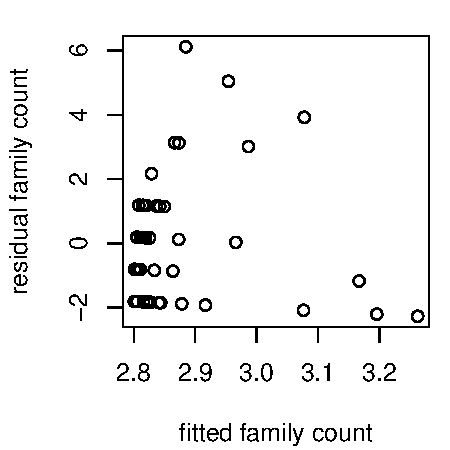
\includegraphics[width=\textwidth]{plots/mass-vs-count/residual/2015_sweep_Diptera_residual.pdf}
		\label{fig:sweep_diptera_resid}
	\end{subfigure}
	~
	\begin{subfigure}[b]{0.15\textwidth}
		\caption{Residual probability}
		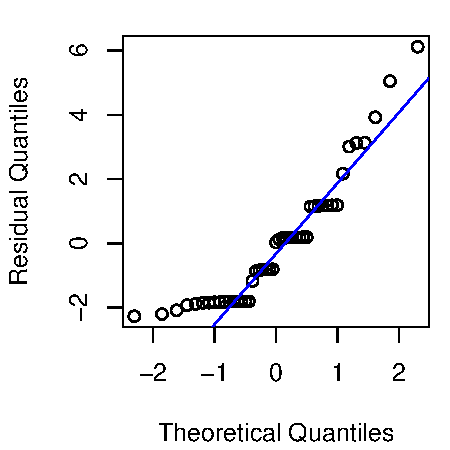
\includegraphics[width=\textwidth]{plots/mass-vs-count/qqplot/2015_sweep_Diptera_qqplot.pdf}
		\label{fig:sweep_diptera_qqplot}
	\end{subfigure}
	\caption{\textbf{(a)}~Scatter plot showing effect of sample mass on family count in sweep samples for order Diptera, with line of best fit (blue), \textbf{(b)}~scatter plot of fitted values and residuals, and \textbf{(c)}~normal probability plot of the residuals.}
	\label{fig:sweep_diptera}
	\smallskip
	\nointerlineskip
	\hrulefill
\end{figure}

\begin{figure}[h]
	\lstset{numbers=left}
	\lstset{xleftmargin=5mm,framexleftmargin=5mm}
	\begin{lstlisting}
sweep Diptera
Call:
lm(formula = temp.frame)

Residuals:
    Min      1Q  Median      3Q     Max 
-2.2625 -1.8044  0.0337  1.1606  6.1154 

Coefficients:
            Estimate Std. Error t value Pr(>|t|)    
(Intercept)   2.7986     0.3565    7.85 5.71e-10 ***
temp.mass     5.5168    14.9188    0.37    0.713    
---
Signif. codes:  0 '***' 0.001 '**' 0.01 '*' 0.05 '.' 0.1 ' ' 1

Residual standard error: 2.026 on 45 degrees of freedom
Multiple R-squared:  0.00303,	Adjusted R-squared:  -0.01913 
F-statistic: 0.1367 on 1 and 45 DF,  p-value: 0.7133
	\end{lstlisting}
	\caption{Verbatim R output of the results of linear regression of family count on sample mass in sweep samples for Diptera.}
	\label{fig:sweep_diptera_regression}
	\smallskip
	\nointerlineskip
	\hrulefill
\end{figure}

\begin{figure}[h]
	\centering
	\begin{subfigure}[b]{0.15\textwidth}
		\caption{Mass vs. families}
		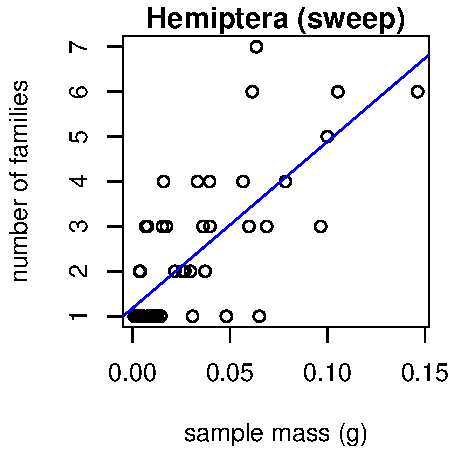
\includegraphics[width=\textwidth]{plots/mass-vs-count/scatter/2015_sweep_Hemiptera_mass-vs-count.pdf}
		\label{fig:sweep_hemiptera_scatter}
	\end{subfigure}
	~
	\begin{subfigure}[b]{0.15\textwidth}
		\caption{Residuals}
		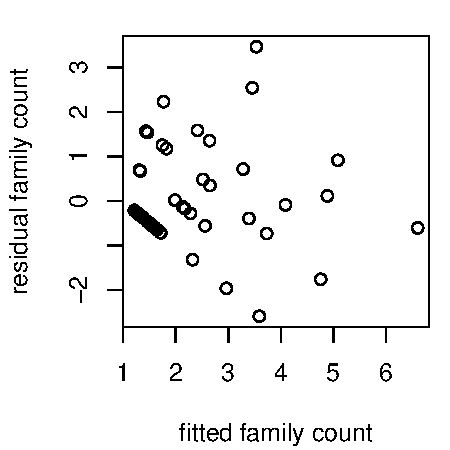
\includegraphics[width=\textwidth]{plots/mass-vs-count/residual/2015_sweep_Hemiptera_residual.pdf}
		\label{fig:sweep_hemiptera_resid}
	\end{subfigure}
	~
	\begin{subfigure}[b]{0.15\textwidth}
		\caption{Residual probability}
		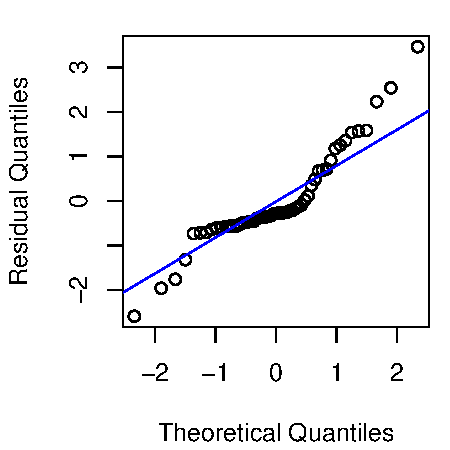
\includegraphics[width=\textwidth]{plots/mass-vs-count/qqplot/2015_sweep_Hemiptera_qqplot.pdf}
		\label{fig:sweep_hemiptera_qqplot}
	\end{subfigure}
	\caption{\textbf{(a)}~Scatter plot showing effect of sample mass on family count in sweep samples for order Hemiptera, with line of best fit (blue), \textbf{(b)}~scatter plot of fitted values and residuals, and \textbf{(c)}~normal probability plot of the residuals.}
	\label{fig:sweep_hemiptera}
	\smallskip
	\nointerlineskip
	\hrulefill
\end{figure}

\begin{figure}[h]
	\lstset{numbers=left}
	\lstset{xleftmargin=5mm,framexleftmargin=5mm}
	\begin{lstlisting}
sweep Hemiptera
Call:
lm(formula = temp.frame)

Residuals:
    Min      1Q  Median      3Q     Max 
-2.5914 -0.5607 -0.2798  0.5293  3.4642 

Coefficients:
            Estimate Std. Error t value Pr(>|t|)    
(Intercept)   1.1747     0.2048   5.735 5.63e-07 ***
temp.mass    37.1234     4.7404   7.831 3.04e-10 ***
---
Signif. codes:  0 '***' 0.001 '**' 0.01 '*' 0.05 '.' 0.1 ' ' 1

Residual standard error: 1.096 on 50 degrees of freedom
Multiple R-squared:  0.5509,	Adjusted R-squared:  0.5419 
F-statistic: 61.33 on 1 and 50 DF,  p-value: 3.035e-10
	\end{lstlisting}
	\caption{Verbatim R output of the results of linear regression of family count on sample mass in sweep samples for Hemiptera.}
	\label{fig:sweep_hemiptera_regression}
	\smallskip
	\nointerlineskip
	\hrulefill
\end{figure}

\begin{figure}[h]
	\centering
	\begin{subfigure}[b]{0.15\textwidth}
		\caption{Mass vs. families}
		\includegraphics[width=\textwidth]{plots/mass-vs-count/scatter/2015_sweep_Hymenoptera_mass-vs-count.pdf}
		\label{fig:sweep_hymenoptera_scatter}
	\end{subfigure}
	~
	\begin{subfigure}[b]{0.15\textwidth}
		\caption{Residuals}
		\includegraphics[width=\textwidth]{plots/mass-vs-count/residual/2015_sweep_Hymenoptera_residual.pdf}
		\label{fig:sweep_hymenoptera_resid}
	\end{subfigure}
	~
	\begin{subfigure}[b]{0.15\textwidth}
		\caption{Residual probability}
		\includegraphics[width=\textwidth]{plots/mass-vs-count/qqplot/2015_sweep_Hymenoptera_qqplot.pdf}
		\label{fig:sweep_hymenoptera_qqplot}
	\end{subfigure}
	\caption{\textbf{(a)}~Scatter plot showing effect of sample mass on family count in sweep samples for order Hymenoptera, with line of best fit (blue), \textbf{(b)}~scatter plot of fitted values and residuals, and \textbf{(c)}~normal probability plot of the residuals.}
	\label{fig:sweep_hymenoptera}
	\smallskip
	\nointerlineskip
	\hrulefill
\end{figure}

\begin{figure}[h]
	\lstset{numbers=left}
	\lstset{xleftmargin=5mm,framexleftmargin=5mm}
	\begin{lstlisting}
sweep Hymenoptera
Call:
lm(formula = temp.frame)

Residuals:
    Min      1Q  Median      3Q     Max 
-1.9558 -0.6956 -0.5165  0.3885  3.3265 

Coefficients:
            Estimate Std. Error t value Pr(>|t|)    
(Intercept)   1.5096     0.2032   7.428 1.08e-08 ***
temp.mass    68.8648    11.5647   5.955 8.86e-07 ***
---
Signif. codes:  0 '***' 0.001 '**' 0.01 '*' 0.05 '.' 0.1 ' ' 1

Residual standard error: 1.104 on 35 degrees of freedom
Multiple R-squared:  0.5033,	Adjusted R-squared:  0.4891 
F-statistic: 35.46 on 1 and 35 DF,  p-value: 8.857e-07
	\end{lstlisting}
	\caption{Verbatim R output of the results of linear regression of family count on sample mass in sweep samples for Hymenoptera.}
	\label{fig:sweep_hymenoptera_regression}
	\smallskip
	\nointerlineskip
	\hrulefill
\end{figure}

\begin{figure}[h]
	\centering
	\begin{subfigure}[b]{0.15\textwidth}
		\caption{Mass vs. families}
		\includegraphics[width=\textwidth]{plots/mass-vs-count/scatter/2015_sweep_Lepidoptera_mass-vs-count.pdf}
		\label{fig:sweep_lepidoptera_scatter}
	\end{subfigure}
	~
	\begin{subfigure}[b]{0.15\textwidth}
		\caption{Residuals}
		\includegraphics[width=\textwidth]{plots/mass-vs-count/residual/2015_sweep_Lepidoptera_residual.pdf}
		\label{fig:sweep_lepidoptera_resid}
	\end{subfigure}
	~
	\begin{subfigure}[b]{0.15\textwidth}
		\caption{Residual probability}
		\includegraphics[width=\textwidth]{plots/mass-vs-count/qqplot/2015_sweep_Lepidoptera_qqplot.pdf}
		\label{fig:sweep_lepidoptera_qqplot}
	\end{subfigure}
	\caption{\textbf{(a)}~Scatter plot showing effect of sample mass on family count in sweep samples for order Lepidoptera, with line of best fit (blue), \textbf{(b)}~scatter plot of fitted values and residuals, and \textbf{(c)}~normal probability plot of the residuals.}
	\label{fig:sweep_lepidoptera}
	\smallskip
	\nointerlineskip
	\hrulefill
\end{figure}

\begin{figure}[h]
	\lstset{numbers=left}
	\lstset{xleftmargin=5mm,framexleftmargin=5mm}
	\begin{lstlisting}
sweep Lepidoptera
Call:
lm(formula = temp.frame)

Residuals:
         1          2          3          4          5          6 
 4.516e-16 -9.691e-17 -9.674e-17 -9.649e-17 -9.800e-17 -6.343e-17 

Coefficients:
              Estimate Std. Error    t value Pr(>|t|)    
(Intercept)  1.000e+00  1.196e-16  8.359e+15   <2e-16 ***
temp.mass   -8.350e-16  6.865e-15 -1.220e-01    0.909    
---
Signif. codes:  0 '***' 0.001 '**' 0.01 '*' 0.05 '.' 0.1 ' ' 1

Residual standard error: 2.478e-16 on 4 degrees of freedom
Multiple R-squared:  0.4127,	Adjusted R-squared:  0.2658 
F-statistic:  2.81 on 1 and 4 DF,  p-value: 0.169
	\end{lstlisting}
	\caption{Verbatim R output of the results of linear regression of family count on sample mass in sweep samples for Lepidoptera.}
	\label{fig:sweep_lepidoptera_regression}
	\smallskip
	\nointerlineskip
	\hrulefill
\end{figure}

\begin{figure}[h]
	\centering
	\begin{subfigure}[b]{0.15\textwidth}
		\caption{Mass vs. families}
		\includegraphics[width=\textwidth]{plots/mass-vs-count/scatter/2015_sweep_Orthoptera_mass-vs-count.pdf}
		\label{fig:sweep_orthoptera_scatter}
	\end{subfigure}
	~
	\begin{subfigure}[b]{0.15\textwidth}
		\caption{Residuals}
		\includegraphics[width=\textwidth]{plots/mass-vs-count/residual/2015_sweep_Orthoptera_residual.pdf}
		\label{fig:sweep_orthoptera_resid}
	\end{subfigure}
	~
	\begin{subfigure}[b]{0.15\textwidth}
		\caption{Residual probability}
		\includegraphics[width=\textwidth]{plots/mass-vs-count/qqplot/2015_sweep_Orthoptera_qqplot.pdf}
		\label{fig:sweep_orthoptera_qqplot}
	\end{subfigure}
	\caption{\textbf{(a)}~Scatter plot showing effect of sample mass on family count in sweep samples for order Orthoptera, with line of best fit (blue), \textbf{(b)}~scatter plot of fitted values and residuals, and \textbf{(c)}~normal probability plot of the residuals.}
	\label{fig:sweep_orthoptera}
	\smallskip
	\nointerlineskip
	\hrulefill
\end{figure}

\begin{figure}[h]
	\lstset{numbers=left}
	\lstset{xleftmargin=5mm,framexleftmargin=5mm}
	\begin{lstlisting}
sweep Orthoptera
Call:
lm(formula = temp.frame)

Residuals:
       Min         1Q     Median         3Q        Max 
-2.534e-16 -9.662e-17 -5.256e-17 -2.899e-17  2.544e-15 

Coefficients:
             Estimate Std. Error   t value Pr(>|t|)    
(Intercept) 1.000e+00  1.169e-16 8.553e+15   <2e-16 ***
temp.mass   2.234e-15  2.835e-15 7.880e-01    0.436    
---
Signif. codes:  0 '***' 0.001 '**' 0.01 '*' 0.05 '.' 0.1 ' ' 1

Residual standard error: 4.465e-16 on 34 degrees of freedom
Multiple R-squared:  0.5032,	Adjusted R-squared:  0.4886 
F-statistic: 34.44 on 1 and 34 DF,  p-value: 1.277e-06
	\end{lstlisting}
	\caption{Verbatim R output of the results of linear regression of family count on sample mass in sweep samples for Orthoptera.}
	\label{fig:sweep_orthoptera_regression}
	\smallskip
	\nointerlineskip
	\hrulefill
\end{figure}

\begin{figure}[h]
	\centering
	\begin{subfigure}[b]{0.15\textwidth}
		\caption{Mass vs. families}
		\includegraphics[width=\textwidth]{plots/mass-vs-count/scatter/2015_sweep_Collembola_mass-vs-count.pdf}
		\label{fig:sweep_collembola_scatter}
	\end{subfigure}
	~
	\begin{subfigure}[b]{0.15\textwidth}
		\caption{Mass vs. families}
		\includegraphics[width=\textwidth]{plots/mass-vs-count/scatter/2015_sweep_Neuroptera_mass-vs-count.pdf}
		\label{fig:sweep_neuroptera_scatter}
	\end{subfigure}
	~
	\begin{subfigure}[b]{0.15\textwidth}
		\caption{Mass vs. families}
		\includegraphics[width=\textwidth]{plots/mass-vs-count/scatter/2015_sweep_Thysanoptera_mass-vs-count.pdf}
		\label{fig:sweep_thysanoptera_scatter}
	\end{subfigure}
	\caption{Scatter plot showing effect of sample mass on family count in sweep samples: \textbf{(a)}~Collembola, \textbf{(b)}~Mantodea, \textbf{(c)}~Neuroptera, \textbf{(d)}~Thysanoptera.}
	\label{fig:sweep_incomplete}
	\smallskip
	\nointerlineskip
	\hrulefill
\end{figure}

\clearpage
\newpage

\section{General linear mixed-effects model}\label{sec:glmm}
To better examine the relationship between sample mass and family diversity, a general linear mixed-effecs model can be used to account for the non-normal distribution of the family count and dry weight data.
Because the family diversity of a sample is a form of count data, a Poisson distribution can be used to model the data within a simple GLMM (\cref{fig:glmm_poisson}).
This model features family count as the dependent variable, with insect order as a random effect, sampling method as a random effect, and sample mass as a fixed effect.
Because the Poisson distribution assumes a variance equal to the mean, while the GLMM has a deviance greater than the degrees of freedom, the model is over-dispersed and likely has a slightly biased variance.
Thus a model based on negative binomial distribution (\cref{fig:glmm,fig:glmm_nb}), of which the Poisson distribution is a special case, can be used to better fit the data; see likelihood ratio test in \cref{fig:glmm_lrt}.
In both models, mass is a significant fixed effect; removal of any effect, random or fixed, produces a significantly less likely fit to the data, indicating that the sampling method and insect order has a significant effect on the relationship between family diversity and sample mass within each test group (\cref{fig:glmm_nb_lrt}).

\begin{figure}[h]
	\centering
	\begin{subfigure}[b]{0.23\textwidth}
		\caption{Residuals}
		\includegraphics[width=\textwidth]{plots/glmm/2015_glmm_residual.pdf}
		\label{fig:glmm_resid}
	\end{subfigure}
	~
	\begin{subfigure}[b]{0.23\textwidth}
		\caption{Residual probability}
		\includegraphics[width=\textwidth]{plots/glmm/2015_glmm_qqplot.pdf}
		\label{fig:glmm_qqplot}
	\end{subfigure}
	\caption{\textbf{General linear mixed-effects model based on negative binomial distribution: (a)}~scatter plot of fitted values and residuals, and \textbf{(b)}~normal probability plot of the residuals.}
	\label{fig:glmm}
	\nointerlineskip
	\hrulefill
\end{figure}

\begin{figure}[h]
	\lstset{numbers=left}
	\lstset{xleftmargin=5mm,framexleftmargin=5mm}
	\begin{lstlisting}
Generalized linear mixed model fit by maximum likelihood (Laplace Approximation) [glmerMod]
 Family: poisson  ( log )
Formula: family_count ~ mass + (1 | order) + (1 | method)
   Data: raw.data[with(raw.data, mass > 0 & family_count > 0), ]

     AIC      BIC   logLik deviance df.resid 
  3578.9   3598.3  -1785.5   3570.9      942 

Scaled residuals: 
    Min      1Q  Median      3Q     Max 
-3.3270 -0.6659 -0.1349  0.4582  4.9910 

Random effects:
 Groups Name        Variance Std.Dev.
 order  (Intercept) 0.3794   0.6159  
 method (Intercept) 0.1502   0.3875  
Number of obs: 946, groups:  order, 11; method, 3

Fixed effects:
            Estimate Std. Error z value Pr(>|z|)    
(Intercept)  0.59879    0.29918   2.001   0.0453 *  
mass         0.19436    0.01227  15.834   <2e-16 ***
---
Signif. codes:  0 '***' 0.001 '**' 0.01 '*' 0.05 '.' 0.1 ' ' 1

Correlation of Fixed Effects:
     (Intr)
mass -0.008
	\end{lstlisting}
	\caption{Verbatim R output of the results of fitting a general linear mixed-effects model based on a Poisson distribution.}
	\label{fig:glmm_poisson}
	\smallskip
	\nointerlineskip
	\hrulefill
\end{figure}

\begin{figure}[h]
	\lstset{numbers=left}
	\lstset{xleftmargin=5mm,framexleftmargin=5mm}
	\begin{lstlisting}
Generalized linear mixed model fit by maximum likelihood (Laplace Approximation) [glmerMod]
 Family: Negative Binomial(43.7543)  ( log )
Formula: family_count ~ mass + (1 | order) + (1 | method)
   Data: raw.data[with(raw.data, mass > 0 & family_count > 0), ]

     AIC      BIC   logLik deviance df.resid 
  3574.0   3598.3  -1782.0   3564.0      941 

Scaled residuals: 
    Min      1Q  Median      3Q     Max 
-2.9952 -0.6286 -0.1483  0.4291  4.7868 

Random effects:
 Groups Name        Variance Std.Dev.
 order  (Intercept) 0.3727   0.6105  
 method (Intercept) 0.1402   0.3744  
Number of obs: 946, groups:  order, 11; method, 3

Fixed effects:
            Estimate Std. Error z value Pr(>|z|)    
(Intercept)   0.6010     0.2929   2.052   0.0402 *  
mass          0.2068     0.0145  14.263   <2e-16 ***
---
Signif. codes:  0 '***' 0.001 '**' 0.01 '*' 0.05 '.' 0.1 ' ' 1

Correlation of Fixed Effects:
     (Intr)
mass -0.009
	\end{lstlisting}
	\caption{Verbatim R output of the results of fitting a general linear mixed-effects model based on a negative binomial distribution (\texttheta~=~43.75).}
	\label{fig:glmm_nb}
	\smallskip
	\nointerlineskip
	\hrulefill
\end{figure}

\begin{figure}[h]
	\lstset{numbers=left}
	\lstset{xleftmargin=5mm,framexleftmargin=5mm}
	\begin{lstlisting}
Likelihood ratio test

Model 1: family_count ~ mass + (1 | order) + (1 | method)
Model 2: family_count ~ mass + (1 | order) + (1 | method)
  #Df  LogLik Df  Chisq Pr(>Chisq)   
1   4 -1785.5                        
2   5 -1782.0  1 6.8946   0.008646 **
---
Signif. codes:  0 '***' 0.001 '**' 0.01 '*' 0.05 '.' 0.1 ' ' 1
	\end{lstlisting}
	\caption{Likelihood ration test comparing general linear mixed-effects models based on \textbf{1} Poisson and \textbf{2} negative binomial distributions, respectively.}
	\label{fig:glmm_lrt}
	\smallskip
	\nointerlineskip
	\hrulefill
\end{figure}

\begin{figure}[h]
	\lstset{numbers=left}
	\lstset{xleftmargin=5mm,framexleftmargin=5mm}
	\begin{lstlisting}
Likelihood ratio test

Model 1: family_count ~ mass + (1 | order) + (1 | method)
Model 2: family_count ~ (1 | order) + (1 | method)
Model 3: family_count ~ mass + (1 | method)
Model 4: family_count ~ mass + (1 | order)
  #Df  LogLik Df  Chisq Pr(>Chisq)    
1   5 -1782.0                         
2   4 -1865.2 -1 166.26  < 2.2e-16 ***
3   4 -2108.4  0 486.50  < 2.2e-16 ***
4   4 -1878.4  0 460.06  < 2.2e-16 ***
---
Signif. codes:  0 '***' 0.001 '**' 0.01 '*' 0.05 '.' 0.1 ' ' 1
	\end{lstlisting}
	\caption{Verbatim R output of the results of linear regression of family count on sample mass in sweep samples for Orthoptera.}
	\label{fig:glmm_nb_lrt}
	\smallskip
	\nointerlineskip
	\hrulefill
\end{figure}

\clearpage
\newpage

\section{Mass and family count between blocks}\label{sec:blocks}
Statistical exploration of the differences between treatment blocks and sampling dates in terms of sample mass and family level diversity was undertaken using two-way analyses of variance.
These were conducted individually for both dependent variables, for each sampling method and insect order, with sampling week crossed by treatment block as the factors of the ANOVA.
Overall, there are very few differences between the site-wise means within each block and date, although the block and sampling date terms (and their interaction) were frequently significant, indicating a possible random effect from these factors.

In this section, all of the interaction plots for sample mass and family count plots are shown along with summary and test statistics for each ANOVA, including a Shapiro-Wilk test of normality for each comparison.
Although the assumption of normality is nearly always rejected, Levine tests on this data (and bulk data, see \cref{sec:bulk}) suggest that the samples are homoscedastic.
Because the ANOVA is robust to violations of the assumption of normality (as long as the data exhibit equal variance), this test was used for ease of use and interpretability.
Tukey-Kramer tests for multiple comparisons are additionally provided for each ANOVA, along with graphical representation of test results (beginning at \cref{fig:malaise_mass_tukey}).

%MALAISE SAMPLES
\begin{figure}[h]
	\centering
	\begin{subfigure}[b]{0.45\textwidth}
		\caption{Order mass}
		\includegraphics[width=\textwidth]{plots/blocks/interaction/mass/mass_malaise_Coleoptera_interplot.pdf}
		\label{fig:malaise_coleoptera_mass_interplot}
	\end{subfigure}
	~
	\begin{subfigure}[b]{0.45\textwidth}
		\caption{Family count}
		\includegraphics[width=\textwidth]{plots/blocks/interaction/family/family_malaise_Coleoptera_interplot.pdf}
		\label{fig:malaise_coleoptera_family_interplot}
	\end{subfigure}
	\caption{Interaction plot of \textbf{(a)}~sample mass and \textbf{(b)}~family count for order Coleoptera, between treatment blocks and sampling dates.}
	\label{fig:malaise_coleoptera_interplot}
	\smallskip
	\nointerlineskip
	\hrulefill
\end{figure}

\begin{figure}[h]
	\lstset{numbers=left}
	\lstset{xleftmargin=5mm,framexleftmargin=5mm}
	\begin{lstlisting}
Coleoptera malaise 

sample mass 

            Df  Sum Sq  Mean Sq F value Pr(>F)
block        3 0.00390 0.001300   0.325  0.807
event        4 0.02126 0.005315   1.328  0.276
block:event 12 0.03952 0.003293   0.823  0.627
Residuals   40 0.16008 0.004002               
	\end{lstlisting}
	\caption{Verbatim R output of the results of an ANOVA of sample mass in malaise samples for Coleoptera.}
	\label{fig:malaise_coleoptera_mass_anova}
	\smallskip
	\nointerlineskip
	\hrulefill
\end{figure}

\begin{figure}[h]
	\lstset{numbers=left}
	\lstset{xleftmargin=5mm,framexleftmargin=5mm}
	\begin{lstlisting}
Levene's Test for Homogeneity of Variance (center = median)
      Df F value Pr(>F)
group 19  0.9036 0.5818
      40               
	\end{lstlisting}
	\caption{Verbatim R output of the results of Levene's test on sample mass in malaise samples for Coleoptera.}
	\label{fig:malaise_coleoptera_mass_levene}
	\smallskip
	\nointerlineskip
	\hrulefill
\end{figure}

\begin{figure}[h]
	\lstset{numbers=left}
	\lstset{xleftmargin=5mm,framexleftmargin=5mm}
	\begin{lstlisting}
	Shapiro-Wilk normality test

data:  residuals(mass.model)
W = 0.71139, p-value = 1.48e-09
	\end{lstlisting}
	\caption{Verbatim R output of the results of Shapiro-Wilk's test on sample mass in malaise samples for Coleoptera.}
	\label{fig:malaise_coleoptera_mass_shapiro}
	\smallskip
	\nointerlineskip
	\hrulefill
\end{figure}

\begin{figure}[h]
	\lstset{numbers=left}
	\lstset{xleftmargin=5mm,framexleftmargin=5mm}
	\begin{lstlisting}
sample families 

            Df Sum Sq Mean Sq F value Pr(>F)  
block        3   8.73   2.911   2.646 0.0621 .
event        4   6.17   1.542   1.402 0.2510  
block:event 12  13.43   1.119   1.018 0.4517  
Residuals   40  44.00   1.100                 
---
Signif. codes:  0 '***' 0.001 '**' 0.01 '*' 0.05 '.' 0.1 ' ' 1
	\end{lstlisting}
	\caption{Verbatim R output of the results of an ANOVA of family count in malaise samples for Coleoptera.}
	\label{fig:malaise_coleoptera_family_anova}
	\smallskip
	\nointerlineskip
	\hrulefill
\end{figure}

\begin{figure}[h]
	\lstset{numbers=left}
	\lstset{xleftmargin=5mm,framexleftmargin=5mm}
	\begin{lstlisting}
Levene's Test for Homogeneity of Variance (center = median)
      Df F value Pr(>F)
group 19  0.5775 0.9004
      40               
	\end{lstlisting}
	\caption{Verbatim R output of the results of Levene's test on family count in malaise samples for Coleoptera.}
	\label{fig:malaise_coleoptera_family_levene}
	\smallskip
	\nointerlineskip
	\hrulefill
\end{figure}

\begin{figure}[h]
	\lstset{numbers=left}
	\lstset{xleftmargin=5mm,framexleftmargin=5mm}
	\begin{lstlisting}
	Shapiro-Wilk normality test

data:  residuals(family.model)
W = 0.95706, p-value = 0.03386
	\end{lstlisting}
	\caption{Verbatim R output of the results of Shapiro-Wilk's test on family count in malaise samples for Coleoptera.}
	\label{fig:malaise_coleoptera_family_shapiro}
	\smallskip
	\nointerlineskip
	\hrulefill
\end{figure}

\begin{figure}[h]
	\centering
	\begin{subfigure}[b]{0.45\textwidth}
		\caption{Order mass}
		\includegraphics[width=\textwidth]{plots/blocks/interaction/mass/mass_malaise_Diptera_interplot.pdf}
		\label{fig:malaise_diptera_mass_interplot}
	\end{subfigure}
	~
	\begin{subfigure}[b]{0.45\textwidth}
		\caption{Family count}
		\includegraphics[width=\textwidth]{plots/blocks/interaction/family/family_malaise_Diptera_interplot.pdf}
		\label{fig:malaise_diptera_family_interplot}
	\end{subfigure}
	\caption{Interaction plot of \textbf{(a)}~sample mass and \textbf{(b)}~family count for order Diptera, between treatment blocks and sampling dates.}
	\label{fig:malaise_diptera_interplot}
	\smallskip
	\nointerlineskip
	\hrulefill
\end{figure}

\begin{figure}[h]
	\lstset{numbers=left}
	\lstset{xleftmargin=5mm,framexleftmargin=5mm}
	\begin{lstlisting}
Diptera malaise 

sample mass 

            Df Sum Sq Mean Sq F value   Pr(>F)    
block        3 14.425   4.808   8.760 0.000138 ***
event        4  1.672   0.418   0.762 0.556401    
block:event 12  6.944   0.579   1.054 0.421957    
Residuals   40 21.956   0.549                     
---
Signif. codes:  0 '***' 0.001 '**' 0.01 '*' 0.05 '.' 0.1 ' ' 1
	\end{lstlisting}
	\caption{Verbatim R output of the results of an ANOVA of sample mass in malaise samples for Diptera.}
	\label{fig:malaise_diptera_mass_anova}
	\smallskip
	\nointerlineskip
	\hrulefill
\end{figure}

\begin{figure}[h]
	\lstset{numbers=left}
	\lstset{xleftmargin=5mm,framexleftmargin=5mm}
	\begin{lstlisting}
Levene's Test for Homogeneity of Variance (center = median)
      Df F value Pr(>F)
group 19  0.9248 0.5591
      40               
	\end{lstlisting}
	\caption{Verbatim R output of the results of Levene's test on sample mass in malaise samples for Diptera.}
	\label{fig:malaise_diptera_mass_levene}
	\smallskip
	\nointerlineskip
	\hrulefill
\end{figure}

\begin{figure}[h]
	\lstset{numbers=left}
	\lstset{xleftmargin=5mm,framexleftmargin=5mm}
	\begin{lstlisting}
	Shapiro-Wilk normality test

data:  residuals(mass.model)
W = 0.90104, p-value = 0.0001435
	\end{lstlisting}
	\caption{Verbatim R output of the results of Shapiro-Wilk's test on sample mass in malaise samples for Diptera.}
	\label{fig:malaise_diptera_mass_shapiro}
	\smallskip
	\nointerlineskip
	\hrulefill
\end{figure}

\begin{figure}[h]
	\lstset{numbers=left}
	\lstset{xleftmargin=5mm,framexleftmargin=5mm}
	\begin{lstlisting}
sample families 

            Df Sum Sq Mean Sq F value  Pr(>F)    
block        3  347.9  115.97   8.921 0.00012 ***
event        4  233.2   58.31   4.485 0.00435 ** 
block:event 12  285.8   23.82   1.832 0.07556 .  
Residuals   40  520.0   13.00                    
---
Signif. codes:  0 '***' 0.001 '**' 0.01 '*' 0.05 '.' 0.1 ' ' 1
	\end{lstlisting}
	\caption{Verbatim R output of the results of an ANOVA of family count in malaise samples for Diptera.}
	\label{fig:malaise_diptera_family_anova}
	\smallskip
	\nointerlineskip
	\hrulefill
\end{figure}

\begin{figure}[h]
	\lstset{numbers=left}
	\lstset{xleftmargin=5mm,framexleftmargin=5mm}
	\begin{lstlisting}
Levene's Test for Homogeneity of Variance (center = median)
      Df F value Pr(>F)
group 19  0.2961  0.997
      40               
	\end{lstlisting}
	\caption{Verbatim R output of the results of Levene's test on family count in malaise samples for Diptera.}
	\label{fig:malaise_diptera_family_levene}
	\smallskip
	\nointerlineskip
	\hrulefill
\end{figure}

\begin{figure}[h]
	\lstset{numbers=left}
	\lstset{xleftmargin=5mm,framexleftmargin=5mm}
	\begin{lstlisting}
	Shapiro-Wilk normality test

data:  residuals(family.model)
W = 0.96916, p-value = 0.1327
	\end{lstlisting}
	\caption{Verbatim R output of the results of Shapiro-Wilk's test on family count in malaise samples for Diptera.}
	\label{fig:malaise_diptera_family_shapiro}
	\smallskip
	\nointerlineskip
	\hrulefill
\end{figure}

\begin{figure}[h]
	\centering
	\begin{subfigure}[b]{0.45\textwidth}
		\caption{Order mass}
		\includegraphics[width=\textwidth]{plots/blocks/interaction/mass/mass_malaise_Hemiptera_interplot.pdf}
		\label{fig:malaise_hemiptera_mass_interplot}
	\end{subfigure}
	~
	\begin{subfigure}[b]{0.45\textwidth}
		\caption{Family count}
		\includegraphics[width=\textwidth]{plots/blocks/interaction/family/family_malaise_Hemiptera_interplot.pdf}
		\label{fig:malaise_hemiptera_family_interplot}
	\end{subfigure}
	\caption{Interaction plot of \textbf{(a)}~sample mass and \textbf{(b)}~family count for order Hemiptera, between treatment blocks and sampling dates.}
	\label{fig:malaise_hemiptera_interplot}
	\smallskip
	\nointerlineskip
	\hrulefill
\end{figure}

\begin{figure}[h]
	\lstset{numbers=left}
	\lstset{xleftmargin=5mm,framexleftmargin=5mm}
	\begin{lstlisting}
Hemiptera malaise 

sample mass 

            Df   Sum Sq   Mean Sq F value  Pr(>F)   
block        3 0.003175 0.0010582   4.385 0.00926 **
event        4 0.004093 0.0010231   4.240 0.00592 **
block:event 12 0.005632 0.0004693   1.945 0.05763 . 
Residuals   40 0.009653 0.0002413                   
---
Signif. codes:  0 '***' 0.001 '**' 0.01 '*' 0.05 '.' 0.1 ' ' 1
	\end{lstlisting}
	\caption{Verbatim R output of the results of an ANOVA of sample mass in malaise samples for Hemiptera.}
	\label{fig:malaise_hemiptera_mass_anova}
	\smallskip
	\nointerlineskip
	\hrulefill
\end{figure}

\begin{figure}[h]
	\lstset{numbers=left}
	\lstset{xleftmargin=5mm,framexleftmargin=5mm}
	\begin{lstlisting}
Levene's Test for Homogeneity of Variance (center = median)
      Df F value Pr(>F)
group 19  1.1294 0.3612
      40               
	\end{lstlisting}
	\caption{Verbatim R output of the results of Levene's test on sample mass in malaise samples for Hemiptera.}
	\label{fig:malaise_hemiptera_mass_levene}
	\smallskip
	\nointerlineskip
	\hrulefill
\end{figure}

\begin{figure}[h]
	\lstset{numbers=left}
	\lstset{xleftmargin=5mm,framexleftmargin=5mm}
	\begin{lstlisting}
	Shapiro-Wilk normality test

data:  residuals(mass.model)
W = 0.9128, p-value = 0.0003982
	\end{lstlisting}
	\caption{Verbatim R output of the results of Shapiro-Wilk's test on sample mass in malaise samples for Hemiptera.}
	\label{fig:malaise_hemiptera_mass_shapiro}
	\smallskip
	\nointerlineskip
	\hrulefill
\end{figure}

\begin{figure}[h]
	\lstset{numbers=left}
	\lstset{xleftmargin=5mm,framexleftmargin=5mm}
	\begin{lstlisting}
sample families 

            Df Sum Sq Mean Sq F value Pr(>F)  
block        3  13.38   4.461   3.569 0.0223 *
event        4  10.23   2.558   2.047 0.1061  
block:event 12   8.03   0.669   0.536 0.8783  
Residuals   40  50.00   1.250                 
---
Signif. codes:  0 '***' 0.001 '**' 0.01 '*' 0.05 '.' 0.1 ' ' 1
	\end{lstlisting}
	\caption{Verbatim R output of the results of an ANOVA of family count in malaise samples for Hemiptera.}
	\label{fig:malaise_hemiptera_family_anova}
	\smallskip
	\nointerlineskip
	\hrulefill
\end{figure}

\begin{figure}[h]
	\lstset{numbers=left}
	\lstset{xleftmargin=5mm,framexleftmargin=5mm}
	\begin{lstlisting}
Levene's Test for Homogeneity of Variance (center = median)
      Df F value Pr(>F)
group 19  0.5895 0.8918
      40               
	\end{lstlisting}
	\caption{Verbatim R output of the results of Levene's test on family count in malaise samples for Hemiptera.}
	\label{fig:malaise_hemiptera_family_levene}
	\smallskip
	\nointerlineskip
	\hrulefill
\end{figure}

\begin{figure}[h]
	\lstset{numbers=left}
	\lstset{xleftmargin=5mm,framexleftmargin=5mm}
	\begin{lstlisting}
	Shapiro-Wilk normality test

data:  residuals(family.model)
W = 0.95788, p-value = 0.03711
	\end{lstlisting}
	\caption{Verbatim R output of the results of Shapiro-Wilk's test on family count in malaise samples for Hemiptera.}
	\label{fig:malaise_hemiptera_family_shapiro}
	\smallskip
	\nointerlineskip
	\hrulefill
\end{figure}

\begin{figure}[h]
	\centering
	\begin{subfigure}[b]{0.45\textwidth}
		\caption{Order mass}
		\includegraphics[width=\textwidth]{plots/blocks/interaction/mass/mass_malaise_Hymenoptera_interplot.pdf}
		\label{fig:malaise_hymenoptera_mass_interplot}
	\end{subfigure}
	~
	\begin{subfigure}[b]{0.45\textwidth}
		\caption{Family count}
		\includegraphics[width=\textwidth]{plots/blocks/interaction/family/family_malaise_Hymenoptera_interplot.pdf}
		\label{fig:malaise_hymenoptera_family_interplot}
	\end{subfigure}
	\caption{Interaction plot of \textbf{(a)}~sample mass and \textbf{(b)}~family count for order Hymenoptera, between treatment blocks and sampling dates.}
	\label{fig:malaise_hymenoptera_interplot}
	\smallskip
	\nointerlineskip
	\hrulefill
\end{figure}

\begin{figure}[h]
	\lstset{numbers=left}
	\lstset{xleftmargin=5mm,framexleftmargin=5mm}
	\begin{lstlisting}
Hymenoptera malaise 

sample mass 

            Df Sum Sq Mean Sq F value   Pr(>F)    
block        3  4.461   1.487   4.664  0.00717 ** 
event        4 19.282   4.821  15.120 1.76e-07 ***
block:event 11  7.109   0.646   2.027  0.05285 .  
Residuals   38 12.115   0.319                     
---
Signif. codes:  0 '***' 0.001 '**' 0.01 '*' 0.05 '.' 0.1 ' ' 1
	\end{lstlisting}
	\caption{Verbatim R output of the results of an ANOVA of sample mass in malaise samples for Hymenoptera.}
	\label{fig:malaise_hymenoptera_mass_anova}
	\smallskip
	\nointerlineskip
	\hrulefill
\end{figure}

\begin{figure}[h]
	\lstset{numbers=left}
	\lstset{xleftmargin=5mm,framexleftmargin=5mm}
	\begin{lstlisting}
Levene's Test for Homogeneity of Variance (center = median)
      Df F value Pr(>F)
group 18  1.4405 0.1687
      38               
	\end{lstlisting}
	\caption{Verbatim R output of the results of Levene's test on sample mass in malaise samples for Hymenoptera.}
	\label{fig:malaise_hymenoptera_mass_levene}
	\smallskip
	\nointerlineskip
	\hrulefill
\end{figure}

\begin{figure}[h]
	\lstset{numbers=left}
	\lstset{xleftmargin=5mm,framexleftmargin=5mm}
	\begin{lstlisting}
	Shapiro-Wilk normality test

data:  residuals(mass.model)
W = 0.87674, p-value = 3.171e-05
	\end{lstlisting}
	\caption{Verbatim R output of the results of Shapiro-Wilk's test on sample mass in malaise samples for Hymenoptera.}
	\label{fig:malaise_hymenoptera_mass_shapiro}
	\smallskip
	\nointerlineskip
	\hrulefill
\end{figure}

\begin{figure}[h]
	\lstset{numbers=left}
	\lstset{xleftmargin=5mm,framexleftmargin=5mm}
	\begin{lstlisting}
sample families 

            Df Sum Sq Mean Sq F value  Pr(>F)   
block        3  25.87   8.623   5.285 0.00381 **
event        4   5.77   1.443   0.884 0.48247   
block:event 11  22.08   2.007   1.230 0.30151   
Residuals   38  62.00   1.632                   
---
Signif. codes:  0 '***' 0.001 '**' 0.01 '*' 0.05 '.' 0.1 ' ' 1
	\end{lstlisting}
	\caption{Verbatim R output of the results of an ANOVA of family count in malaise samples for Hymenoptera.}
	\label{fig:malaise_hymenoptera_family_anova}
	\smallskip
	\nointerlineskip
	\hrulefill
\end{figure}

\begin{figure}[h]
	\lstset{numbers=left}
	\lstset{xleftmargin=5mm,framexleftmargin=5mm}
	\begin{lstlisting}
Levene's Test for Homogeneity of Variance (center = median)
      Df F value Pr(>F)
group 18  0.6691 0.8185
      38               
	\end{lstlisting}
	\caption{Verbatim R output of the results of Levene's test on family count in malaise samples for Hymenoptera.}
	\label{fig:malaise_hymenoptera_family_levene}
	\smallskip
	\nointerlineskip
	\hrulefill
\end{figure}

\begin{figure}[h]
	\lstset{numbers=left}
	\lstset{xleftmargin=5mm,framexleftmargin=5mm}
	\begin{lstlisting}
	Shapiro-Wilk normality test

data:  residuals(family.model)
W = 0.97428, p-value = 0.2638
	\end{lstlisting}
	\caption{Verbatim R output of the results of Shapiro-Wilk's test on family count in malaise samples for Hymenoptera.}
	\label{fig:malaise_hymenoptera_family_shapiro}
	\smallskip
	\nointerlineskip
	\hrulefill
\end{figure}

\begin{figure}[h]
	\centering
	\begin{subfigure}[b]{0.45\textwidth}
		\caption{Order mass}
		\includegraphics[width=\textwidth]{plots/blocks/interaction/mass/mass_malaise_Lepidoptera_interplot.pdf}
		\label{fig:malaise_lepidoptera_mass_interplot}
	\end{subfigure}
	~
	\begin{subfigure}[b]{0.45\textwidth}
		\caption{Family count}
		\includegraphics[width=\textwidth]{plots/blocks/interaction/family/family_malaise_Lepidoptera_interplot.pdf}
		\label{fig:malaise_lepidoptera_family_interplot}
	\end{subfigure}
	\caption{Interaction plot of \textbf{(a)}~sample mass and \textbf{(b)}~family count for order Lepidoptera, between treatment blocks and sampling dates.}
	\label{fig:malaise_lepidoptera_interplot}
	\smallskip
	\nointerlineskip
	\hrulefill
\end{figure}

\begin{figure}[h]
	\lstset{numbers=left}
	\lstset{xleftmargin=5mm,framexleftmargin=5mm}
	\begin{lstlisting}
Lepidoptera malaise 

sample mass 

            Df Sum Sq Mean Sq F value Pr(>F)  
block        3 0.5074 0.16914   2.928 0.0453 *
event        4 0.0975 0.02438   0.422 0.7918  
block:event 12 0.7560 0.06300   1.090 0.3938  
Residuals   40 2.3111 0.05778                 
---
Signif. codes:  0 '***' 0.001 '**' 0.01 '*' 0.05 '.' 0.1 ' ' 1
	\end{lstlisting}
	\caption{Verbatim R output of the results of an ANOVA of sample mass in malaise samples for Lepidoptera.}
	\label{fig:malaise_lepidoptera_mass_anova}
	\smallskip
	\nointerlineskip
	\hrulefill
\end{figure}

\begin{figure}[h]
	\lstset{numbers=left}
	\lstset{xleftmargin=5mm,framexleftmargin=5mm}
	\begin{lstlisting}
Levene's Test for Homogeneity of Variance (center = median)
      Df F value Pr(>F)
group 19  0.8305 0.6609
      40               
	\end{lstlisting}
	\caption{Verbatim R output of the results of Levene's test on sample mass in malaise samples for Lepidoptera.}
	\label{fig:malaise_lepidoptera_mass_levene}
	\smallskip
	\nointerlineskip
	\hrulefill
\end{figure}

\begin{figure}[h]
	\lstset{numbers=left}
	\lstset{xleftmargin=5mm,framexleftmargin=5mm}
	\begin{lstlisting}
	Shapiro-Wilk normality test

data:  residuals(mass.model)
W = 0.79655, p-value = 1.108e-07
	\end{lstlisting}
	\caption{Verbatim R output of the results of Shapiro-Wilk's test on sample mass in malaise samples for Lepidoptera.}
	\label{fig:malaise_lepidoptera_mass_shapiro}
	\smallskip
	\nointerlineskip
	\hrulefill
\end{figure}

\begin{figure}[h]
	\lstset{numbers=left}
	\lstset{xleftmargin=5mm,framexleftmargin=5mm}
	\begin{lstlisting}
sample families 

            Df Sum Sq Mean Sq F value Pr(>F)   
block        3  4.983   1.661   3.020 0.0408 * 
event        4  4.167   1.042   1.894 0.1304   
block:event 12 19.433   1.619   2.944 0.0051 **
Residuals   40 22.000   0.550                  
---
Signif. codes:  0 '***' 0.001 '**' 0.01 '*' 0.05 '.' 0.1 ' ' 1
	\end{lstlisting}
	\caption{Verbatim R output of the results of an ANOVA of family count in malaise samples for Lepidoptera.}
	\label{fig:malaise_lepidoptera_family_anova}
	\smallskip
	\nointerlineskip
	\hrulefill
\end{figure}

\begin{figure}[h]
	\lstset{numbers=left}
	\lstset{xleftmargin=5mm,framexleftmargin=5mm}
	\begin{lstlisting}
Levene's Test for Homogeneity of Variance (center = median)
      Df F value Pr(>F)
group 19  0.6238 0.8651
      40               
	\end{lstlisting}
	\caption{Verbatim R output of the results of Levene's test on family count in malaise samples for Lepidoptera.}
	\label{fig:malaise_lepidoptera_family_levene}
	\smallskip
	\nointerlineskip
	\hrulefill
\end{figure}

\begin{figure}[h]
	\lstset{numbers=left}
	\lstset{xleftmargin=5mm,framexleftmargin=5mm}
	\begin{lstlisting}
	Shapiro-Wilk normality test

data:  residuals(family.model)
W = 0.92346, p-value = 0.00106
	\end{lstlisting}
	\caption{Verbatim R output of the results of Shapiro-Wilk's test on family count in malaise samples for Lepidoptera.}
	\label{fig:malaise_lepidoptera_family_shapiro}
	\smallskip
	\nointerlineskip
	\hrulefill
\end{figure}

\begin{figure}[h]
	\centering
	\begin{subfigure}[b]{0.45\textwidth}
		\caption{Order mass}
		\includegraphics[width=\textwidth]{plots/blocks/interaction/mass/mass_malaise_Orthoptera_interplot.pdf}
		\label{fig:malaise_orthoptera_mass_interplot}
	\end{subfigure}
	~
	\begin{subfigure}[b]{0.45\textwidth}
		\caption{Family count}
		\includegraphics[width=\textwidth]{plots/blocks/interaction/family/family_malaise_Orthoptera_interplot.pdf}
		\label{fig:malaise_orthoptera_family_interplot}
	\end{subfigure}
	\caption{Interaction plot of \textbf{(a)}~sample mass and \textbf{(b)}~family count for order Orthoptera, between treatment blocks and sampling dates.}
	\label{fig:malaise_orthoptera_interplot}
	\smallskip
	\nointerlineskip
	\hrulefill
\end{figure}

\begin{figure}[h]
	\lstset{numbers=left}
	\lstset{xleftmargin=5mm,framexleftmargin=5mm}
	\begin{lstlisting}
Orthoptera malaise 

sample mass 

            Df Sum Sq Mean Sq F value   Pr(>F)    
block        3 0.3408 0.11360   5.729  0.00233 ** 
event        4 1.1013 0.27532  13.886 3.46e-07 ***
block:event 12 0.1174 0.00979   0.494  0.90629    
Residuals   40 0.7931 0.01983                     
---
Signif. codes:  0 '***' 0.001 '**' 0.01 '*' 0.05 '.' 0.1 ' ' 1
	\end{lstlisting}
	\caption{Verbatim R output of the results of an ANOVA of sample mass in malaise samples for Orthoptera.}
	\label{fig:malaise_orthoptera_mass_anova}
	\smallskip
	\nointerlineskip
	\hrulefill
\end{figure}

\begin{figure}[h]
	\lstset{numbers=left}
	\lstset{xleftmargin=5mm,framexleftmargin=5mm}
	\begin{lstlisting}
Levene's Test for Homogeneity of Variance (center = median)
      Df F value Pr(>F)
group 19  0.6022 0.8823
      40               
	\end{lstlisting}
	\caption{Verbatim R output of the results of Levene's test on sample mass in malaise samples for Orthoptera.}
	\label{fig:malaise_orthoptera_mass_levene}
	\smallskip
	\nointerlineskip
	\hrulefill
\end{figure}

\begin{figure}[h]
	\lstset{numbers=left}
	\lstset{xleftmargin=5mm,framexleftmargin=5mm}
	\begin{lstlisting}
	Shapiro-Wilk normality test

data:  residuals(mass.model)
W = 0.97762, p-value = 0.3365
	\end{lstlisting}
	\caption{Verbatim R output of the results of Shapiro-Wilk's test on sample mass in malaise samples for Orthoptera.}
	\label{fig:malaise_orthoptera_mass_shapiro}
	\smallskip
	\nointerlineskip
	\hrulefill
\end{figure}

\begin{figure}[h]
	\lstset{numbers=left}
	\lstset{xleftmargin=5mm,framexleftmargin=5mm}
	\begin{lstlisting}
sample families 

            Df Sum Sq Mean Sq F value  Pr(>F)   
block        3  4.850  1.6167   5.389 0.00328 **
event        4  6.233  1.5583   5.194 0.00182 **
block:event 12  4.567  0.3806   1.269 0.27430   
Residuals   40 12.000  0.3000                   
---
Signif. codes:  0 '***' 0.001 '**' 0.01 '*' 0.05 '.' 0.1 ' ' 1
	\end{lstlisting}
	\caption{Verbatim R output of the results of an ANOVA of family count in malaise samples for Orthoptera.}
	\label{fig:malaise_orthoptera_family_anova}
	\smallskip
	\nointerlineskip
	\hrulefill
\end{figure}

\begin{figure}[h]
	\lstset{numbers=left}
	\lstset{xleftmargin=5mm,framexleftmargin=5mm}
	\begin{lstlisting}
Levene's Test for Homogeneity of Variance (center = median)
      Df F value Pr(>F)
group 19  0.5099 0.9419
      40               
	\end{lstlisting}
	\caption{Verbatim R output of the results of Levene's test on family count in malaise samples for Orthoptera.}
	\label{fig:malaise_orthoptera_family_levene}
	\smallskip
	\nointerlineskip
	\hrulefill
\end{figure}

\begin{figure}[h]
	\lstset{numbers=left}
	\lstset{xleftmargin=5mm,framexleftmargin=5mm}
	\begin{lstlisting}
	Shapiro-Wilk normality test

data:  residuals(family.model)
W = 0.92188, p-value = 0.0009135
	\end{lstlisting}
	\caption{Verbatim R output of the results of Shapiro-Wilk's test on family count in malaise samples for Orthoptera.}
	\label{fig:malaise_orthoptera_family_shapiro}
	\smallskip
	\nointerlineskip
	\hrulefill
\end{figure}

\begin{figure}[h]
	\centering
	\begin{subfigure}[b]{0.45\textwidth}
		\caption{Order mass}
		\includegraphics[width=\textwidth]{plots/blocks/interaction/mass/mass_malaise_Neuroptera_interplot.pdf}
		\label{fig:malaise_neuroptera_mass_interplot}
	\end{subfigure}
	~
	\begin{subfigure}[b]{0.45\textwidth}
		\caption{Family count}
		\includegraphics[width=\textwidth]{plots/blocks/interaction/family/family_malaise_Neuroptera_interplot.pdf}
		\label{fig:malaise_neuroptera_family_interplot}
	\end{subfigure}
	\caption{Interaction plot of \textbf{(a)}~sample mass and \textbf{(b)}~family count for order Neuroptera, between treatment blocks and sampling dates.}
	\label{fig:malaise_neuroptera_interplot}
	\smallskip
	\nointerlineskip
	\hrulefill
\end{figure}

\begin{figure}[h]
	\lstset{numbers=left}
	\lstset{xleftmargin=5mm,framexleftmargin=5mm}
	\begin{lstlisting}
Neuroptera malaise 

sample mass 

            Df    Sum Sq   Mean Sq F value Pr(>F)
block        3 0.0000429 1.430e-05   1.506  0.228
event        4 0.0000246 6.159e-06   0.649  0.631
block:event 12 0.0001382 1.152e-05   1.213  0.308
Residuals   40 0.0003797 9.493e-06               
	\end{lstlisting}
	\caption{Verbatim R output of the results of an ANOVA of sample mass in malaise samples for Neuroptera.}
	\label{fig:malaise_neuroptera_mass_anova}
	\smallskip
	\nointerlineskip
	\hrulefill
\end{figure}

\begin{figure}[h]
	\lstset{numbers=left}
	\lstset{xleftmargin=5mm,framexleftmargin=5mm}
	\begin{lstlisting}
Levene's Test for Homogeneity of Variance (center = median)
      Df F value Pr(>F)
group 19  0.4473 0.9689
      40               
	\end{lstlisting}
	\caption{Verbatim R output of the results of Levene's test on sample mass in malaise samples for Neuroptera.}
	\label{fig:malaise_neuroptera_mass_levene}
	\smallskip
	\nointerlineskip
	\hrulefill
\end{figure}

\begin{figure}[h]
	\lstset{numbers=left}
	\lstset{xleftmargin=5mm,framexleftmargin=5mm}
	\begin{lstlisting}
	Shapiro-Wilk normality test

data:  residuals(mass.model)
W = 0.96538, p-value = 0.0865
	\end{lstlisting}
	\caption{Verbatim R output of the results of Shapiro-Wilk's test on sample mass in malaise samples for Neuroptera.}
	\label{fig:malaise_neuroptera_mass_shapiro}
	\smallskip
	\nointerlineskip
	\hrulefill
\end{figure}

\begin{figure}[h]
	\lstset{numbers=left}
	\lstset{xleftmargin=5mm,framexleftmargin=5mm}
	\begin{lstlisting}
sample families 

            Df Sum Sq Mean Sq F value Pr(>F)  
block        3  3.533  1.1778   2.524 0.0713 .
event        4  4.267  1.0667   2.286 0.0769 .
block:event 12  3.467  0.2889   0.619 0.8132  
Residuals   40 18.667  0.4667                 
---
Signif. codes:  0 '***' 0.001 '**' 0.01 '*' 0.05 '.' 0.1 ' ' 1
	\end{lstlisting}
	\caption{Verbatim R output of the results of an ANOVA of family count in malaise samples for Neuroptera.}
	\label{fig:malaise_neuroptera_family_anova}
	\smallskip
	\nointerlineskip
	\hrulefill
\end{figure}

\begin{figure}[h]
	\lstset{numbers=left}
	\lstset{xleftmargin=5mm,framexleftmargin=5mm}
	\begin{lstlisting}
Levene's Test for Homogeneity of Variance (center = median)
      Df F value Pr(>F)
group 19  0.6316 0.8587
      40               
	\end{lstlisting}
	\caption{Verbatim R output of the results of Levene's test on family count in malaise samples for Neuroptera.}
	\label{fig:malaise_neuroptera_family_levene}
	\smallskip
	\nointerlineskip
	\hrulefill
\end{figure}

\begin{figure}[h]
	\lstset{numbers=left}
	\lstset{xleftmargin=5mm,framexleftmargin=5mm}
	\begin{lstlisting}
	Shapiro-Wilk normality test

data:  residuals(family.model)
W = 0.93234, p-value = 0.002499
	\end{lstlisting}
	\caption{Verbatim R output of the results of Shapiro-Wilk's test on family count in malaise samples for Neuroptera.}
	\label{fig:malaise_neuroptera_family_shapiro}
	\smallskip
	\nointerlineskip
	\hrulefill
\end{figure}

%PITFALL SAMPLES
\begin{figure}[h]
	\centering
	\begin{subfigure}[b]{0.45\textwidth}
		\caption{Order mass}
		\includegraphics[width=\textwidth]{plots/blocks/interaction/mass/mass_pitfall_Coleoptera_interplot.pdf}
		\label{fig:pitfall_coleoptera_mass_interplot}
	\end{subfigure}
	~
	\begin{subfigure}[b]{0.45\textwidth}
		\caption{Family count}
		\includegraphics[width=\textwidth]{plots/blocks/interaction/family/family_pitfall_Coleoptera_interplot.pdf}
		\label{fig:pitfall_coleoptera_family_interplot}
	\end{subfigure}
	\caption{Interaction plot of \textbf{(a)}~sample mass and \textbf{(b)}~family count for order Coleoptera, between treatment blocks and sampling dates.}
	\label{fig:pitfall_coleoptera_interplot}
	\smallskip
	\nointerlineskip
	\hrulefill
\end{figure}

\begin{figure}[h]
	\lstset{numbers=left}
	\lstset{xleftmargin=5mm,framexleftmargin=5mm}
	\begin{lstlisting}
Coleoptera pitfall 

sample mass 

            Df Sum Sq Mean Sq F value Pr(>F)  
block        3  34.16  11.388   2.845 0.0496 *
event        4  33.86   8.465   2.115 0.0968 .
block:event 12  49.49   4.124   1.031 0.4411  
Residuals   40 160.09   4.002                 
---
Signif. codes:  0 '***' 0.001 '**' 0.01 '*' 0.05 '.' 0.1 ' ' 1   
	\end{lstlisting}
	\caption{Verbatim R output of the results of an ANOVA of sample mass in pitfall samples for Coleoptera.}
	\label{fig:pitfall_coleoptera_mass_anova}
	\smallskip
	\nointerlineskip
	\hrulefill
\end{figure}

\begin{figure}[h]
	\lstset{numbers=left}
	\lstset{xleftmargin=5mm,framexleftmargin=5mm}
	\begin{lstlisting}
Levene's Test for Homogeneity of Variance (center = median)
      Df F value Pr(>F)
group 19  0.9862 0.4952
      40               
	\end{lstlisting}
	\caption{Verbatim R output of the results of Levene's test on sample mass in pitfall samples for Coleoptera.}
	\label{fig:pitfall_coleoptera_mass_levene}
	\smallskip
	\nointerlineskip
	\hrulefill
\end{figure}

\begin{figure}[h]
	\lstset{numbers=left}
	\lstset{xleftmargin=5mm,framexleftmargin=5mm}
	\begin{lstlisting}
	Shapiro-Wilk normality test

data:  residuals(mass.model)
W = 0.93552, p-value = 0.003434
	\end{lstlisting}
	\caption{Verbatim R output of the results of Shapiro-Wilk's test on sample mass in pitfall samples for Coleoptera.}
	\label{fig:pitfall_coleoptera_mass_shapiro}
	\smallskip
	\nointerlineskip
	\hrulefill
\end{figure}

\begin{figure}[h]
	\lstset{numbers=left}
	\lstset{xleftmargin=5mm,framexleftmargin=5mm}
	\begin{lstlisting}
sample families 

            Df Sum Sq Mean Sq F value Pr(>F)
block        3  11.52   3.839   0.601  0.618
event        4  52.43  13.108   2.054  0.105
block:event 12  90.90   7.575   1.187  0.325
Residuals   40 255.33   6.383               
	\end{lstlisting}
	\caption{Verbatim R output of the results of an ANOVA of family count in pitfall samples for Coleoptera.}
	\label{fig:pitfall_coleoptera_family_anova}
	\smallskip
	\nointerlineskip
	\hrulefill
\end{figure}

\begin{figure}[h]
	\lstset{numbers=left}
	\lstset{xleftmargin=5mm,framexleftmargin=5mm}
	\begin{lstlisting}
Levene's Test for Homogeneity of Variance (center = median)
      Df F value Pr(>F)
group 19  0.3518 0.9915
      40               
	\end{lstlisting}
	\caption{Verbatim R output of the results of Levene's test on family count in pitfall samples for Coleoptera.}
	\label{fig:pitfall_coleoptera_family_levene}
	\smallskip
	\nointerlineskip
	\hrulefill
\end{figure}

\begin{figure}[h]
	\lstset{numbers=left}
	\lstset{xleftmargin=5mm,framexleftmargin=5mm}
	\begin{lstlisting}
	Shapiro-Wilk normality test

data:  residuals(family.model)
W = 0.98591, p-value = 0.7174
	\end{lstlisting}
	\caption{Verbatim R output of the results of Shapiro-Wilk's test on family count in pitfall samples for Coleoptera.}
	\label{fig:pitfall_coleoptera_family_shapiro}
	\smallskip
	\nointerlineskip
	\hrulefill
\end{figure}

\begin{figure}[h]
	\centering
	\begin{subfigure}[b]{0.45\textwidth}
		\caption{Order mass}
		\includegraphics[width=\textwidth]{plots/blocks/interaction/mass/mass_pitfall_Diptera_interplot.pdf}
		\label{fig:pitfall_diptera_mass_interplot}
	\end{subfigure}
	~
	\begin{subfigure}[b]{0.45\textwidth}
		\caption{Family count}
		\includegraphics[width=\textwidth]{plots/blocks/interaction/family/family_pitfall_Diptera_interplot.pdf}
		\label{fig:pitfall_diptera_family_interplot}
	\end{subfigure}
	\caption{Interaction plot of \textbf{(a)}~sample mass and \textbf{(b)}~family count for order Diptera, between treatment blocks and sampling dates.}
	\label{fig:pitfall_diptera_interplot}
	\smallskip
	\nointerlineskip
	\hrulefill
\end{figure}

\begin{figure}[h]
	\lstset{numbers=left}
	\lstset{xleftmargin=5mm,framexleftmargin=5mm}
	\begin{lstlisting}
Diptera pitfall 

sample mass 

            Df Sum Sq Mean Sq F value Pr(>F)  
block        3 0.0402 0.01341   1.058 0.3778  
event        4 0.1607 0.04018   3.170 0.0236 *
block:event 12 0.2720 0.02266   1.788 0.0840 .
Residuals   40 0.5070 0.01268                 
---
Signif. codes:  0 '***' 0.001 '**' 0.01 '*' 0.05 '.' 0.1 ' ' 1
	\end{lstlisting}
	\caption{Verbatim R output of the results of an ANOVA of sample mass in pitfall samples for Diptera.}
	\label{fig:pitfall_diptera_mass_anova}
	\smallskip
	\nointerlineskip
	\hrulefill
\end{figure}

\begin{figure}[h]
	\lstset{numbers=left}
	\lstset{xleftmargin=5mm,framexleftmargin=5mm}
	\begin{lstlisting}
Levene's Test for Homogeneity of Variance (center = median)
      Df F value Pr(>F)
group 19  0.7445 0.7521
      40               
	\end{lstlisting}
	\caption{Verbatim R output of the results of Levene's test on sample mass in pitfall samples for Diptera.}
	\label{fig:pitfall_diptera_mass_levene}
	\smallskip
	\nointerlineskip
	\hrulefill
\end{figure}

\begin{figure}[h]
	\lstset{numbers=left}
	\lstset{xleftmargin=5mm,framexleftmargin=5mm}
	\begin{lstlisting}
	Shapiro-Wilk normality test

data:  residuals(mass.model)
W = 0.94508, p-value = 0.0092
	\end{lstlisting}
	\caption{Verbatim R output of the results of Shapiro-Wilk's test on sample mass in pitfall samples for Diptera.}
	\label{fig:pitfall_diptera_mass_shapiro}
	\smallskip
	\nointerlineskip
	\hrulefill
\end{figure}

\begin{figure}[h]
	\lstset{numbers=left}
	\lstset{xleftmargin=5mm,framexleftmargin=5mm}
	\begin{lstlisting}
sample families 

            Df Sum Sq Mean Sq F value Pr(>F)   
block        3  26.93   8.978   2.181 0.1053   
event        4  67.27  16.817   4.085 0.0072 **
block:event 12  78.07   6.506   1.580 0.1369   
Residuals   40 164.67   4.117                  
---
Signif. codes:  0 '***' 0.001 '**' 0.01 '*' 0.05 '.' 0.1 ' ' 1
	\end{lstlisting}
	\caption{Verbatim R output of the results of an ANOVA of family count in pitfall samples for Diptera.}
	\label{fig:pitfall_diptera_family_anova}
	\smallskip
	\nointerlineskip
	\hrulefill
\end{figure}

\begin{figure}[h]
	\lstset{numbers=left}
	\lstset{xleftmargin=5mm,framexleftmargin=5mm}
	\begin{lstlisting}
Levene's Test for Homogeneity of Variance (center = median)
      Df F value Pr(>F)
group 19  0.6766 0.8189
      40               
	\end{lstlisting}
	\caption{Verbatim R output of the results of Levene's test on family count in pitfall samples for Diptera.}
	\label{fig:pitfall_diptera_family_levene}
	\smallskip
	\nointerlineskip
	\hrulefill
\end{figure}

\begin{figure}[h]
	\lstset{numbers=left}
	\lstset{xleftmargin=5mm,framexleftmargin=5mm}
	\begin{lstlisting}
	Shapiro-Wilk normality test

data:  residuals(family.model)
W = 0.96611, p-value = 0.09394
	\end{lstlisting}
	\caption{Verbatim R output of the results of Shapiro-Wilk's test on family count in pitfall samples for Diptera.}
	\label{fig:pitfall_diptera_family_shapiro}
	\smallskip
	\nointerlineskip
	\hrulefill
\end{figure}

\begin{figure}[h]
	\centering
	\begin{subfigure}[b]{0.45\textwidth}
		\caption{Order mass}
		\includegraphics[width=\textwidth]{plots/blocks/interaction/mass/mass_pitfall_Hemiptera_interplot.pdf}
		\label{fig:pitfall_hemiptera_mass_interplot}
	\end{subfigure}
	~
	\begin{subfigure}[b]{0.45\textwidth}
		\caption{Family count}
		\includegraphics[width=\textwidth]{plots/blocks/interaction/family/family_pitfall_Hemiptera_interplot.pdf}
		\label{fig:pitfall_hemiptera_family_interplot}
	\end{subfigure}
	\caption{Interaction plot of \textbf{(a)}~sample mass and \textbf{(b)}~family count for order Hemiptera, between treatment blocks and sampling dates.}
	\label{fig:pitfall_hemiptera_interplot}
	\smallskip
	\nointerlineskip
	\hrulefill
\end{figure}

\begin{figure}[h]
	\lstset{numbers=left}
	\lstset{xleftmargin=5mm,framexleftmargin=5mm}
	\begin{lstlisting}
Hemiptera pitfall 

sample mass 

            Df   Sum Sq   Mean Sq F value   Pr(>F)    
block        3 0.002927 0.0009756   5.511   0.0029 ** 
event        4 0.008375 0.0020937  11.828 1.96e-06 ***
block:event 12 0.003863 0.0003219   1.818   0.0781 .  
Residuals   40 0.007080 0.0001770                     
---
Signif. codes:  0 '***' 0.001 '**' 0.01 '*' 0.05 '.' 0.1 ' ' 1
	\end{lstlisting}
	\caption{Verbatim R output of the results of an ANOVA of sample mass in pitfall samples for Hemiptera.}
	\label{fig:pitfall_hemiptera_mass_anova}
	\smallskip
	\nointerlineskip
	\hrulefill
\end{figure}

\begin{figure}[h]
	\lstset{numbers=left}
	\lstset{xleftmargin=5mm,framexleftmargin=5mm}
	\begin{lstlisting}
Levene's Test for Homogeneity of Variance (center = median)
      Df F value Pr(>F)
group 19  0.7198 0.7771
      40               
	\end{lstlisting}
	\caption{Verbatim R output of the results of Levene's test on sample mass in pitfall samples for Hemiptera.}
	\label{fig:pitfall_hemiptera_mass_levene}
	\smallskip
	\nointerlineskip
	\hrulefill
\end{figure}

\begin{figure}[h]
	\lstset{numbers=left}
	\lstset{xleftmargin=5mm,framexleftmargin=5mm}
	\begin{lstlisting}
	Shapiro-Wilk normality test

data:  residuals(mass.model)
W = 0.96982, p-value = 0.143
	\end{lstlisting}
	\caption{Verbatim R output of the results of Shapiro-Wilk's test on sample mass in pitfall samples for Hemiptera.}
	\label{fig:pitfall_hemiptera_mass_shapiro}
	\smallskip
	\nointerlineskip
	\hrulefill
\end{figure}

\begin{figure}[h]
	\lstset{numbers=left}
	\lstset{xleftmargin=5mm,framexleftmargin=5mm}
	\begin{lstlisting}
sample families 

            Df Sum Sq Mean Sq F value Pr(>F)  
block        3   7.78  2.5944   2.638 0.0626 .
event        4   6.77  1.6917   1.720 0.1645  
block:event 12  12.30  1.0250   1.042 0.4315  
Residuals   40  39.33  0.9833                 
---
Signif. codes:  0 '***' 0.001 '**' 0.01 '*' 0.05 '.' 0.1 ' ' 1
	\end{lstlisting}
	\caption{Verbatim R output of the results of an ANOVA of family count in pitfall samples for Hemiptera.}
	\label{fig:pitfall_hemiptera_family_anova}
	\smallskip
	\nointerlineskip
	\hrulefill
\end{figure}

\begin{figure}[h]
	\lstset{numbers=left}
	\lstset{xleftmargin=5mm,framexleftmargin=5mm}
	\begin{lstlisting}
Levene's Test for Homogeneity of Variance (center = median)
      Df F value Pr(>F)
group 19   0.588 0.8929
      40               
	\end{lstlisting}
	\caption{Verbatim R output of the results of Levene's test on family count in pitfall samples for Hemiptera.}
	\label{fig:pitfall_hemiptera_family_levene}
	\smallskip
	\nointerlineskip
	\hrulefill
\end{figure}

\begin{figure}[h]
	\lstset{numbers=left}
	\lstset{xleftmargin=5mm,framexleftmargin=5mm}
	\begin{lstlisting}
	Shapiro-Wilk normality test

data:  residuals(family.model)
W = 0.96595, p-value = 0.09223
	\end{lstlisting}
	\caption{Verbatim R output of the results of Shapiro-Wilk's test on family count in pitfall samples for Hemiptera.}
	\label{fig:pitfall_hemiptera_family_shapiro}
	\smallskip
	\nointerlineskip
	\hrulefill
\end{figure}

\begin{figure}[h]
	\centering
	\begin{subfigure}[b]{0.45\textwidth}
		\caption{Order mass}
		\includegraphics[width=\textwidth]{plots/blocks/interaction/mass/mass_pitfall_Hymenoptera_interplot.pdf}
		\label{fig:pitfall_hymenoptera_mass_interplot}
	\end{subfigure}
	~
	\begin{subfigure}[b]{0.45\textwidth}
		\caption{Family count}
		\includegraphics[width=\textwidth]{plots/blocks/interaction/family/family_pitfall_Hymenoptera_interplot.pdf}
		\label{fig:pitfall_hymenoptera_family_interplot}
	\end{subfigure}
	\caption{Interaction plot of \textbf{(a)}~sample mass and \textbf{(b)}~family count for order Hymenoptera, between treatment blocks and sampling dates.}
	\label{fig:pitfall_hymenoptera_interplot}
	\smallskip
	\nointerlineskip
	\hrulefill
\end{figure}

\begin{figure}[h]
	\lstset{numbers=left}
	\lstset{xleftmargin=5mm,framexleftmargin=5mm}
	\begin{lstlisting}
Hymenoptera pitfall 

sample mass 

            Df   Sum Sq   Mean Sq F value Pr(>F)  
block        3 0.002314 0.0007713   2.119 0.1130  
event        4 0.004349 0.0010873   2.987 0.0301 *
block:event 12 0.006666 0.0005555   1.526 0.1552  
Residuals   40 0.014559 0.0003640                 
---
Signif. codes:  0 '***' 0.001 '**' 0.01 '*' 0.05 '.' 0.1 ' ' 1
	\end{lstlisting}
	\caption{Verbatim R output of the results of an ANOVA of sample mass in pitfall samples for Hymenoptera.}
	\label{fig:pitfall_hymenoptera_mass_anova}
	\smallskip
	\nointerlineskip
	\hrulefill
\end{figure}

\begin{figure}[h]
	\lstset{numbers=left}
	\lstset{xleftmargin=5mm,framexleftmargin=5mm}
	\begin{lstlisting}
Levene's Test for Homogeneity of Variance (center = median)
      Df F value Pr(>F)
group 19  0.8187 0.6736
      40               
	\end{lstlisting}
	\caption{Verbatim R output of the results of Levene's test on sample mass in pitfall samples for Hymenoptera.}
	\label{fig:pitfall_hymenoptera_mass_levene}
	\smallskip
	\nointerlineskip
	\hrulefill
\end{figure}

\begin{figure}[h]
	\lstset{numbers=left}
	\lstset{xleftmargin=5mm,framexleftmargin=5mm}
	\begin{lstlisting}
	Shapiro-Wilk normality test

data:  residuals(mass.model)
W = 0.94321, p-value = 0.007554
	\end{lstlisting}
	\caption{Verbatim R output of the results of Shapiro-Wilk's test on sample mass in pitfall samples for Hymenoptera.}
	\label{fig:pitfall_hymenoptera_mass_shapiro}
	\smallskip
	\nointerlineskip
	\hrulefill
\end{figure}

\begin{figure}[h]
	\lstset{numbers=left}
	\lstset{xleftmargin=5mm,framexleftmargin=5mm}
	\begin{lstlisting}
sample families 

            Df Sum Sq Mean Sq F value Pr(>F)
block        3  12.45   4.150   1.227  0.313
event        4  20.27   5.067   1.498  0.221
block:event 12  34.80   2.900   0.857  0.594
Residuals   40 135.33   3.383               
	\end{lstlisting}
	\caption{Verbatim R output of the results of an ANOVA of family count in pitfall samples for Hymenoptera.}
	\label{fig:pitfall_hymenoptera_family_anova}
	\smallskip
	\nointerlineskip
	\hrulefill
\end{figure}

\begin{figure}[h]
	\lstset{numbers=left}
	\lstset{xleftmargin=5mm,framexleftmargin=5mm}
	\begin{lstlisting}
Levene's Test for Homogeneity of Variance (center = median)
      Df F value Pr(>F)
group 19  0.6173 0.8704
      40               
	\end{lstlisting}
	\caption{Verbatim R output of the results of Levene's test on family count in pitfall samples for Hymenoptera.}
	\label{fig:pitfall_hymenoptera_family_levene}
	\smallskip
	\nointerlineskip
	\hrulefill
\end{figure}

\begin{figure}[h]
	\lstset{numbers=left}
	\lstset{xleftmargin=5mm,framexleftmargin=5mm}
	\begin{lstlisting}
	Shapiro-Wilk normality test

data:  residuals(family.model)
W = 0.90267, p-value = 0.0001649
	\end{lstlisting}
	\caption{Verbatim R output of the results of Shapiro-Wilk's test on family count in pitfall samples for Hymenoptera.}
	\label{fig:pitfall_hymenoptera_family_shapiro}
	\smallskip
	\nointerlineskip
	\hrulefill
\end{figure}

\begin{figure}[h]
	\centering
	\begin{subfigure}[b]{0.45\textwidth}
		\caption{Order mass}
		\includegraphics[width=\textwidth]{plots/blocks/interaction/mass/mass_pitfall_Lepidoptera_interplot.pdf}
		\label{fig:pitfall_lepidoptera_mass_interplot}
	\end{subfigure}
	~
	\begin{subfigure}[b]{0.45\textwidth}
		\caption{Family count}
		\includegraphics[width=\textwidth]{plots/blocks/interaction/family/family_pitfall_Lepidoptera_interplot.pdf}
		\label{fig:pitfall_lepidoptera_family_interplot}
	\end{subfigure}
	\caption{Interaction plot of \textbf{(a)}~sample mass and \textbf{(b)}~family count for order Lepidoptera, between treatment blocks and sampling dates.}
	\label{fig:pitfall_lepidoptera_interplot}
	\smallskip
	\nointerlineskip
	\hrulefill
\end{figure}

\begin{figure}[h]
	\lstset{numbers=left}
	\lstset{xleftmargin=5mm,framexleftmargin=5mm}
	\begin{lstlisting}
Lepidoptera pitfall 

sample mass 

            Df  Sum Sq  Mean Sq F value Pr(>F)  
block        3 0.00855 0.002849   1.627  0.198  
event        4 0.01607 0.004017   2.294  0.076 .
block:event 12 0.03299 0.002749   1.570  0.140  
Residuals   40 0.07004 0.001751                 
---
Signif. codes:  0 '***' 0.001 '**' 0.01 '*' 0.05 '.' 0.1 ' ' 1
	\end{lstlisting}
	\caption{Verbatim R output of the results of an ANOVA of sample mass in pitfall samples for Lepidoptera.}
	\label{fig:pitfall_lepidoptera_mass_anova}
	\smallskip
	\nointerlineskip
	\hrulefill
\end{figure}

\begin{figure}[h]
	\lstset{numbers=left}
	\lstset{xleftmargin=5mm,framexleftmargin=5mm}
	\begin{lstlisting}
Levene's Test for Homogeneity of Variance (center = median)
      Df F value  Pr(>F)  
group 19  1.8073 0.05717 .
      40                  
---
Signif. codes:  0 '***' 0.001 '**' 0.01 '*' 0.05 '.' 0.1 ' ' 1
	\end{lstlisting}
	\caption{Verbatim R output of the results of Levene's test on sample mass in pitfall samples for Lepidoptera.}
	\label{fig:pitfall_lepidoptera_mass_levene}
	\smallskip
	\nointerlineskip
	\hrulefill
\end{figure}

\begin{figure}[h]
	\lstset{numbers=left}
	\lstset{xleftmargin=5mm,framexleftmargin=5mm}
	\begin{lstlisting}
	Shapiro-Wilk normality test

data:  residuals(mass.model)
W = 0.73291, p-value = 4.04e-09
	\end{lstlisting}
	\caption{Verbatim R output of the results of Shapiro-Wilk's test on sample mass in pitfall samples for Lepidoptera.}
	\label{fig:pitfall_lepidoptera_mass_shapiro}
	\smallskip
	\nointerlineskip
	\hrulefill
\end{figure}

\begin{figure}[h]
	\lstset{numbers=left}
	\lstset{xleftmargin=5mm,framexleftmargin=5mm}
	\begin{lstlisting}
sample families 

            Df Sum Sq Mean Sq F value Pr(>F)
block        3  0.983  0.3278   1.035  0.387
event        4  1.567  0.3917   1.237  0.311
block:event 12  3.767  0.3139   0.991  0.474
Residuals   40 12.667  0.3167               
	\end{lstlisting}
	\caption{Verbatim R output of the results of an ANOVA of family count in pitfall samples for Lepidoptera.}
	\label{fig:pitfall_lepidoptera_family_anova}
	\smallskip
	\nointerlineskip
	\hrulefill
\end{figure}

\begin{figure}[h]
	\lstset{numbers=left}
	\lstset{xleftmargin=5mm,framexleftmargin=5mm}
	\begin{lstlisting}
Levene's Test for Homogeneity of Variance (center = median)
      Df F value Pr(>F)
group 19  0.4596 0.9644
      40               
	\end{lstlisting}
	\caption{Verbatim R output of the results of Levene's test on family count in pitfall samples for Lepidoptera.}
	\label{fig:pitfall_lepidoptera_family_levene}
	\smallskip
	\nointerlineskip
	\hrulefill
\end{figure}

\begin{figure}[h]
	\lstset{numbers=left}
	\lstset{xleftmargin=5mm,framexleftmargin=5mm}
	\begin{lstlisting}
	Shapiro-Wilk normality test

data:  residuals(family.model)
W = 0.95335, p-value = 0.02244
	\end{lstlisting}
	\caption{Verbatim R output of the results of Shapiro-Wilk's test on family count in pitfall samples for Lepidoptera.}
	\label{fig:pitfall_lepidoptera_family_shapiro}
	\smallskip
	\nointerlineskip
	\hrulefill
\end{figure}

\begin{figure}[h]
	\centering
	\begin{subfigure}[b]{0.45\textwidth}
		\caption{Order mass}
		\includegraphics[width=\textwidth]{plots/blocks/interaction/mass/mass_pitfall_Orthoptera_interplot.pdf}
		\label{fig:pitfall_orthoptera_mass_interplot}
	\end{subfigure}
	~
	\begin{subfigure}[b]{0.45\textwidth}
		\caption{Family count}
		\includegraphics[width=\textwidth]{plots/blocks/interaction/family/family_pitfall_Orthoptera_interplot.pdf}
		\label{fig:pitfall_orthoptera_family_interplot}
	\end{subfigure}
	\caption{Interaction plot of \textbf{(a)}~sample mass and \textbf{(b)}~family count for order Orthoptera, between treatment blocks and sampling dates.}
	\label{fig:pitfall_orthoptera_interplot}
	\smallskip
	\nointerlineskip
	\hrulefill
\end{figure}

\begin{figure}[h]
	\lstset{numbers=left}
	\lstset{xleftmargin=5mm,framexleftmargin=5mm}
	\begin{lstlisting}
Orthoptera pitfall 

sample mass 

            Df Sum Sq Mean Sq F value Pr(>F)  
block        3  3.373  1.1243   3.330 0.0289 *
event        4  2.848  0.7120   2.109 0.0976 .
block:event 12  5.054  0.4212   1.247 0.2868  
Residuals   40 13.504  0.3376                 
---
Signif. codes:  0 '***' 0.001 '**' 0.01 '*' 0.05 '.' 0.1 ' ' 1
	\end{lstlisting}
	\caption{Verbatim R output of the results of an ANOVA of sample mass in pitfall samples for Orthoptera.}
	\label{fig:pitfall_orthoptera_mass_anova}
	\smallskip
	\nointerlineskip
	\hrulefill
\end{figure}

\begin{figure}[h]
	\lstset{numbers=left}
	\lstset{xleftmargin=5mm,framexleftmargin=5mm}
	\begin{lstlisting}
Levene's Test for Homogeneity of Variance (center = median)
      Df F value Pr(>F)
group 19   0.743 0.7537
      40               
	\end{lstlisting}
	\caption{Verbatim R output of the results of Levene's test on sample mass in pitfall samples for Orthoptera.}
	\label{fig:pitfall_orthoptera_mass_levene}
	\smallskip
	\nointerlineskip
	\hrulefill
\end{figure}

\begin{figure}[h]
	\lstset{numbers=left}
	\lstset{xleftmargin=5mm,framexleftmargin=5mm}
	\begin{lstlisting}
	Shapiro-Wilk normality test

data:  residuals(mass.model)
W = 0.90797, p-value = 0.00026
	\end{lstlisting}
	\caption{Verbatim R output of the results of Shapiro-Wilk's test on sample mass in pitfall samples for Orthoptera.}
	\label{fig:pitfall_orthoptera_mass_shapiro}
	\smallskip
	\nointerlineskip
	\hrulefill
\end{figure}

\begin{figure}[h]
	\lstset{numbers=left}
	\lstset{xleftmargin=5mm,framexleftmargin=5mm}
	\begin{lstlisting}
sample families 

            Df Sum Sq Mean Sq F value Pr(>F)
block        3   1.80  0.6000   0.655  0.585
event        4   1.77  0.4417   0.482  0.749
block:event 12   2.37  0.1972   0.215  0.997
Residuals   40  36.67  0.9167               
	\end{lstlisting}
	\caption{Verbatim R output of the results of an ANOVA of family count in pitfall samples for Orthoptera.}
	\label{fig:pitfall_orthoptera_family_anova}
	\smallskip
	\nointerlineskip
	\hrulefill
\end{figure}

\begin{figure}[h]
	\lstset{numbers=left}
	\lstset{xleftmargin=5mm,framexleftmargin=5mm}
	\begin{lstlisting}
Levene's Test for Homogeneity of Variance (center = median)
      Df F value Pr(>F)
group 19  0.5098 0.9419
      40               
	\end{lstlisting}
	\caption{Verbatim R output of the results of Levene's test on family count in pitfall samples for Orthoptera.}
	\label{fig:pitfall_orthoptera_family_levene}
	\smallskip
	\nointerlineskip
	\hrulefill
\end{figure}

\begin{figure}[h]
	\lstset{numbers=left}
	\lstset{xleftmargin=5mm,framexleftmargin=5mm}
	\begin{lstlisting}
	Shapiro-Wilk normality test

data:  residuals(family.model)
W = 0.97452, p-value = 0.2412
	\end{lstlisting}
	\caption{Verbatim R output of the results of Shapiro-Wilk's test on family count in pitfall samples for Orthoptera.}
	\label{fig:pitfall_orthoptera_family_shapiro}
	\smallskip
	\nointerlineskip
	\hrulefill
\end{figure}

\begin{figure}[h]
	\centering
	\begin{subfigure}[b]{0.45\textwidth}
		\caption{Order mass}
		\includegraphics[width=\textwidth]{plots/blocks/interaction/mass/mass_pitfall_Neuroptera_interplot.pdf}
		\label{fig:pitfall_neuroptera_mass_interplot}
	\end{subfigure}
	~
	\begin{subfigure}[b]{0.45\textwidth}
		\caption{Family count}
		\includegraphics[width=\textwidth]{plots/blocks/interaction/family/family_pitfall_Neuroptera_interplot.pdf}
		\label{fig:pitfall_neuroptera_family_interplot}
	\end{subfigure}
	\caption{Interaction plot of \textbf{(a)}~sample mass and \textbf{(b)}~family count for order Neuroptera, between treatment blocks and sampling dates.}
	\label{fig:pitfall_neuroptera_interplot}
	\smallskip
	\nointerlineskip
	\hrulefill
\end{figure}

\begin{figure}[h]
	\lstset{numbers=left}
	\lstset{xleftmargin=5mm,framexleftmargin=5mm}
	\begin{lstlisting}
Neuroptera pitfall 

sample mass 

            Df    Sum Sq   Mean Sq F value Pr(>F)
block        3 8.470e-06 2.824e-06   1.251  0.304
event        4 6.240e-06 1.561e-06   0.691  0.602
block:event 12 2.075e-05 1.729e-06   0.766  0.680
Residuals   40 9.029e-05 2.257e-06               
	\end{lstlisting}
	\caption{Verbatim R output of the results of an ANOVA of sample mass in pitfall samples for Neuroptera.}
	\label{fig:pitfall_neuroptera_mass_anova}
	\smallskip
	\nointerlineskip
	\hrulefill
\end{figure}

\begin{figure}[h]
	\lstset{numbers=left}
	\lstset{xleftmargin=5mm,framexleftmargin=5mm}
	\begin{lstlisting}
Levene's Test for Homogeneity of Variance (center = median)
      Df F value Pr(>F)
group 19  0.8269 0.6647
      40               
	\end{lstlisting}
	\caption{Verbatim R output of the results of Levene's test on sample mass in pitfall samples for Neuroptera.}
	\label{fig:pitfall_neuroptera_mass_levene}
	\smallskip
	\nointerlineskip
	\hrulefill
\end{figure}

\begin{figure}[h]
	\lstset{numbers=left}
	\lstset{xleftmargin=5mm,framexleftmargin=5mm}
	\begin{lstlisting}
	Shapiro-Wilk normality test

data:  residuals(mass.model)
W = 0.64401, p-value = 8.511e-11
	\end{lstlisting}
	\caption{Verbatim R output of the results of Shapiro-Wilk's test on sample mass in pitfall samples for Neuroptera.}
	\label{fig:pitfall_neuroptera_mass_shapiro}
	\smallskip
	\nointerlineskip
	\hrulefill
\end{figure}

\begin{figure}[h]
	\lstset{numbers=left}
	\lstset{xleftmargin=5mm,framexleftmargin=5mm}
	\begin{lstlisting}
sample families 

            Df Sum Sq Mean Sq F value Pr(>F)
block        3  0.400  0.1333   1.143  0.343
event        4  0.100  0.0250   0.214  0.929
block:event 12  1.767  0.1472   1.262  0.278
Residuals   40  4.667  0.1167               
	\end{lstlisting}
	\caption{Verbatim R output of the results of an ANOVA of family count in pitfall samples for Neuroptera.}
	\label{fig:pitfall_neuroptera_family_anova}
	\smallskip
	\nointerlineskip
	\hrulefill
\end{figure}

\begin{figure}[h]
	\lstset{numbers=left}
	\lstset{xleftmargin=5mm,framexleftmargin=5mm}
	\begin{lstlisting}
Levene's Test for Homogeneity of Variance (center = median)
      Df F value Pr(>F)
group 19  0.6842 0.8117
      40               
	\end{lstlisting}
	\caption{Verbatim R output of the results of Levene's test on family count in pitfall samples for Neuroptera.}
	\label{fig:pitfall_neuroptera_family_levene}
	\smallskip
	\nointerlineskip
	\hrulefill
\end{figure}

\begin{figure}[h]
	\lstset{numbers=left}
	\lstset{xleftmargin=5mm,framexleftmargin=5mm}
	\begin{lstlisting}
	Shapiro-Wilk normality test

data:  residuals(family.model)
W = 0.75545, p-value = 1.225e-08
	\end{lstlisting}
	\caption{Verbatim R output of the results of Shapiro-Wilk's test on family count in pitfall samples for Neuroptera.}
	\label{fig:pitfall_neuroptera_family_shapiro}
	\smallskip
	\nointerlineskip
	\hrulefill
\end{figure}

%SWEEP SAMPLES
\begin{figure}[h]
	\centering
	\begin{subfigure}[b]{0.45\textwidth}
		\caption{Order mass}
		\includegraphics[width=\textwidth]{plots/blocks/interaction/mass/mass_sweep_Coleoptera_interplot.pdf}
		\label{fig:sweep_coleoptera_mass_interplot}
	\end{subfigure}
	~
	\begin{subfigure}[b]{0.45\textwidth}
		\caption{Family count}
		\includegraphics[width=\textwidth]{plots/blocks/interaction/family/family_sweep_Coleoptera_interplot.pdf}
		\label{fig:sweep_coleoptera_family_interplot}
	\end{subfigure}
	\caption{Interaction plot of \textbf{(a)}~sample mass and \textbf{(b)}~family count for order Coleoptera, between treatment blocks and sampling dates.}
	\label{fig:sweep_coleoptera_interplot}
	\smallskip
	\nointerlineskip
	\hrulefill
\end{figure}

\begin{figure}[h]
	\lstset{numbers=left}
	\lstset{xleftmargin=5mm,framexleftmargin=5mm}
	\begin{lstlisting}
Coleoptera sweep 

sample mass 

            Df Sum Sq Mean Sq F value Pr(>F)  
block        3 0.1190 0.03968   2.305 0.0914 .
event        4 0.0549 0.01371   0.797 0.5345  
block:event 12 0.1651 0.01376   0.799 0.6488  
Residuals   40 0.6886 0.01721                 
---
Signif. codes:  0 '***' 0.001 '**' 0.01 '*' 0.05 '.' 0.1 ' ' 1
	\end{lstlisting}
	\caption{Verbatim R output of the results of an ANOVA of sample mass in sweep samples for Coleoptera.}
	\label{fig:sweep_coleoptera_mass_anova}
	\smallskip
	\nointerlineskip
	\hrulefill
\end{figure}

\begin{figure}[h]
	\lstset{numbers=left}
	\lstset{xleftmargin=5mm,framexleftmargin=5mm}
	\begin{lstlisting}
Levene's Test for Homogeneity of Variance (center = median)
      Df F value Pr(>F)
group 19  0.8936 0.5925
      40               
	\end{lstlisting}
	\caption{Verbatim R output of the results of Levene's test on sample mass in sweep samples for Coleoptera.}
	\label{fig:sweep_coleoptera_mass_levene}
	\smallskip
	\nointerlineskip
	\hrulefill
\end{figure}

\begin{figure}[h]
	\lstset{numbers=left}
	\lstset{xleftmargin=5mm,framexleftmargin=5mm}
	\begin{lstlisting}
	Shapiro-Wilk normality test

data:  residuals(mass.model)
W = 0.53431, p-value = 1.641e-12
	\end{lstlisting}
	\caption{Verbatim R output of the results of Shapiro-Wilk's test on sample mass in sweep samples for Coleoptera.}
	\label{fig:sweep_coleoptera_mass_shapiro}
	\smallskip
	\nointerlineskip
	\hrulefill
\end{figure}

\begin{figure}[h]
	\lstset{numbers=left}
	\lstset{xleftmargin=5mm,framexleftmargin=5mm}
	\begin{lstlisting}
sample families 

            Df Sum Sq Mean Sq F value Pr(>F)  
block        3  19.38   6.461   4.038 0.0134 *
event        4  12.23   3.058   1.911 0.1273  
block:event 12   9.37   0.781   0.488 0.9099  
Residuals   40  64.00   1.600                 
---
Signif. codes:  0 '***' 0.001 '**' 0.01 '*' 0.05 '.' 0.1 ' ' 1
	\end{lstlisting}
	\caption{Verbatim R output of the results of an ANOVA of family count in sweep samples for Coleoptera.}
	\label{fig:sweep_coleoptera_family_anova}
	\smallskip
	\nointerlineskip
	\hrulefill
\end{figure}

\begin{figure}[h]
	\lstset{numbers=left}
	\lstset{xleftmargin=5mm,framexleftmargin=5mm}
	\begin{lstlisting}
Levene's Test for Homogeneity of Variance (center = median)
      Df F value Pr(>F)
group 19  0.5263  0.933
      40               
	\end{lstlisting}
	\caption{Verbatim R output of the results of Levene's test on family count in sweep samples for Coleoptera.}
	\label{fig:sweep_coleoptera_family_levene}
	\smallskip
	\nointerlineskip
	\hrulefill
\end{figure}

\begin{figure}[h]
	\lstset{numbers=left}
	\lstset{xleftmargin=5mm,framexleftmargin=5mm}
	\begin{lstlisting}
	Shapiro-Wilk normality test

data:  residuals(family.model)
W = 0.97314, p-value = 0.2073
	\end{lstlisting}
	\caption{Verbatim R output of the results of Shapiro-Wilk's test on family count in sweep samples for Coleoptera.}
	\label{fig:sweep_coleoptera_family_shapiro}
	\smallskip
	\nointerlineskip
	\hrulefill
\end{figure}

\begin{figure}[h]
	\centering
	\begin{subfigure}[b]{0.45\textwidth}
		\caption{Order mass}
		\includegraphics[width=\textwidth]{plots/blocks/interaction/mass/mass_sweep_Diptera_interplot.pdf}
		\label{fig:sweep_diptera_mass_interplot}
	\end{subfigure}
	~
	\begin{subfigure}[b]{0.45\textwidth}
		\caption{Family count}
		\includegraphics[width=\textwidth]{plots/blocks/interaction/family/family_sweep_Diptera_interplot.pdf}
		\label{fig:sweep_diptera_family_interplot}
	\end{subfigure}
	\caption{Interaction plot of \textbf{(a)}~sample mass and \textbf{(b)}~family count for order Diptera, between treatment blocks and sampling dates.}
	\label{fig:sweep_diptera_interplot}
	\smallskip
	\nointerlineskip
	\hrulefill
\end{figure}

\begin{figure}[h]
	\lstset{numbers=left}
	\lstset{xleftmargin=5mm,framexleftmargin=5mm}
	\begin{lstlisting}
Diptera sweep 

sample mass 

            Df   Sum Sq   Mean Sq F value  Pr(>F)   
block        3 0.001383 0.0004610   2.042 0.12342   
event        4 0.001764 0.0004410   1.953 0.12035   
block:event 12 0.007912 0.0006593   2.920 0.00541 **
Residuals   40 0.009031 0.0002258                   
---
Signif. codes:  0 '***' 0.001 '**' 0.01 '*' 0.05 '.' 0.1 ' ' 1
	\end{lstlisting}
	\caption{Verbatim R output of the results of an ANOVA of sample mass in sweep samples for Diptera.}
	\label{fig:sweep_diptera_mass_anova}
	\smallskip
	\nointerlineskip
	\hrulefill
\end{figure}

\begin{figure}[h]
	\lstset{numbers=left}
	\lstset{xleftmargin=5mm,framexleftmargin=5mm}
	\begin{lstlisting}
Levene's Test for Homogeneity of Variance (center = median)
      Df F value Pr(>F)
group 19  1.3753 0.1943
      40               
	\end{lstlisting}
	\caption{Verbatim R output of the results of Levene's test on sample mass in sweep samples for Diptera.}
	\label{fig:sweep_diptera_mass_levene}
	\smallskip
	\nointerlineskip
	\hrulefill
\end{figure}

\begin{figure}[h]
	\lstset{numbers=left}
	\lstset{xleftmargin=5mm,framexleftmargin=5mm}
	\begin{lstlisting}
	Shapiro-Wilk normality test

data:  residuals(mass.model)
W = 0.80278, p-value = 1.585e-07
	\end{lstlisting}
	\caption{Verbatim R output of the results of Shapiro-Wilk's test on sample mass in sweep samples for Diptera.}
	\label{fig:sweep_diptera_mass_shapiro}
	\smallskip
	\nointerlineskip
	\hrulefill
\end{figure}

\begin{figure}[h]
	\lstset{numbers=left}
	\lstset{xleftmargin=5mm,framexleftmargin=5mm}
	\begin{lstlisting}
sample families 

            Df Sum Sq Mean Sq F value  Pr(>F)   
block        3  47.65  15.883   5.606 0.00264 **
event        4  50.50  12.625   4.456 0.00451 **
block:event 12  57.77   4.814   1.699 0.10374   
Residuals   40 113.33   2.833                   
---
Signif. codes:  0 '***' 0.001 '**' 0.01 '*' 0.05 '.' 0.1 ' ' 1
	\end{lstlisting}
	\caption{Verbatim R output of the results of an ANOVA of family count in sweep samples for Diptera.}
	\label{fig:sweep_diptera_family_anova}
	\smallskip
	\nointerlineskip
	\hrulefill
\end{figure}

\begin{figure}[h]
	\lstset{numbers=left}
	\lstset{xleftmargin=5mm,framexleftmargin=5mm}
	\begin{lstlisting}
Levene's Test for Homogeneity of Variance (center = median)
      Df F value Pr(>F)
group 19  1.1484 0.3454
      40               
	\end{lstlisting}
	\caption{Verbatim R output of the results of Levene's test on family count in sweep samples for Diptera.}
	\label{fig:sweep_diptera_family_levene}
	\smallskip
	\nointerlineskip
	\hrulefill
\end{figure}

\begin{figure}[h]
	\lstset{numbers=left}
	\lstset{xleftmargin=5mm,framexleftmargin=5mm}
	\begin{lstlisting}
	Shapiro-Wilk normality test

data:  residuals(family.model)
W = 0.95754, p-value = 0.03571
	\end{lstlisting}
	\caption{Verbatim R output of the results of Shapiro-Wilk's test on family count in sweep samples for Diptera.}
	\label{fig:sweep_diptera_family_shapiro}
	\smallskip
	\nointerlineskip
	\hrulefill
\end{figure}

\begin{figure}[h]
	\centering
	\begin{subfigure}[b]{0.45\textwidth}
		\caption{Order mass}
		\includegraphics[width=\textwidth]{plots/blocks/interaction/mass/mass_sweep_Hemiptera_interplot.pdf}
		\label{fig:sweep_hemiptera_mass_interplot}
	\end{subfigure}
	~
	\begin{subfigure}[b]{0.45\textwidth}
		\caption{Family count}
		\includegraphics[width=\textwidth]{plots/blocks/interaction/family/family_sweep_Hemiptera_interplot.pdf}
		\label{fig:sweep_hemiptera_family_interplot}
	\end{subfigure}
	\caption{Interaction plot of \textbf{(a)}~sample mass and \textbf{(b)}~family count for order Hemiptera, between treatment blocks and sampling dates.}
	\label{fig:sweep_hemiptera_interplot}
	\smallskip
	\nointerlineskip
	\hrulefill
\end{figure}

\begin{figure}[h]
	\lstset{numbers=left}
	\lstset{xleftmargin=5mm,framexleftmargin=5mm}
	\begin{lstlisting}
Hemiptera sweep 

sample mass 

            Df   Sum Sq  Mean Sq F value   Pr(>F)    
block        3 0.005504 0.001835   3.348   0.0284 *  
event        4 0.020188 0.005047   9.209 2.26e-05 ***
block:event 12 0.011767 0.000981   1.789   0.0837 .  
Residuals   40 0.021922 0.000548                     
---
Signif. codes:  0 '***' 0.001 '**' 0.01 '*' 0.05 '.' 0.1 ' ' 1
	\end{lstlisting}
	\caption{Verbatim R output of the results of an ANOVA of sample mass in sweep samples for Hemiptera.}
	\label{fig:sweep_hemiptera_mass_anova}
	\smallskip
	\nointerlineskip
	\hrulefill
\end{figure}

\begin{figure}[h]
	\lstset{numbers=left}
	\lstset{xleftmargin=5mm,framexleftmargin=5mm}
	\begin{lstlisting}
Levene's Test for Homogeneity of Variance (center = median)
      Df F value Pr(>F)
group 19  0.6272 0.8623
      40               
	\end{lstlisting}
	\caption{Verbatim R output of the results of Levene's test on sample mass in sweep samples for Hemiptera.}
	\label{fig:sweep_hemiptera_mass_levene}
	\smallskip
	\nointerlineskip
	\hrulefill
\end{figure}

\begin{figure}[h]
	\lstset{numbers=left}
	\lstset{xleftmargin=5mm,framexleftmargin=5mm}
	\begin{lstlisting}
	Shapiro-Wilk normality test

data:  residuals(mass.model)
W = 0.947, p-value = 0.01129
	\end{lstlisting}
	\caption{Verbatim R output of the results of Shapiro-Wilk's test on sample mass in sweep samples for Hemiptera.}
	\label{fig:sweep_hemiptera_mass_shapiro}
	\smallskip
	\nointerlineskip
	\hrulefill
\end{figure}

\begin{figure}[h]
	\lstset{numbers=left}
	\lstset{xleftmargin=5mm,framexleftmargin=5mm}
	\begin{lstlisting}
sample families 

            Df Sum Sq Mean Sq F value Pr(>F)  
block        3  13.38   4.461   1.821 0.1589  
event        4  22.57   5.642   2.303 0.0752 .
block:event 12  25.03   2.086   0.851 0.5997  
Residuals   40  98.00   2.450                 
---
Signif. codes:  0 '***' 0.001 '**' 0.01 '*' 0.05 '.' 0.1 ' ' 1
	\end{lstlisting}
	\caption{Verbatim R output of the results of an ANOVA of family count in sweep samples for Hemiptera.}
	\label{fig:sweep_hemiptera_family_anova}
	\smallskip
	\nointerlineskip
	\hrulefill
\end{figure}

\begin{figure}[h]
	\lstset{numbers=left}
	\lstset{xleftmargin=5mm,framexleftmargin=5mm}
	\begin{lstlisting}
Levene's Test for Homogeneity of Variance (center = median)
      Df F value Pr(>F)
group 19  0.4906 0.9514
      40               
	\end{lstlisting}
	\caption{Verbatim R output of the results of Levene's test on family count in sweep samples for Hemiptera.}
	\label{fig:sweep_hemiptera_family_levene}
	\smallskip
	\nointerlineskip
	\hrulefill
\end{figure}

\begin{figure}[h]
	\lstset{numbers=left}
	\lstset{xleftmargin=5mm,framexleftmargin=5mm}
	\begin{lstlisting}
	Shapiro-Wilk normality test

data:  residuals(family.model)
W = 0.97236, p-value = 0.1901
	\end{lstlisting}
	\caption{Verbatim R output of the results of Shapiro-Wilk's test on family count in sweep samples for Hemiptera.}
	\label{fig:sweep_hemiptera_family_shapiro}
	\smallskip
	\nointerlineskip
	\hrulefill
\end{figure}

\begin{figure}[h]
	\centering
	\begin{subfigure}[b]{0.45\textwidth}
		\caption{Order mass}
		\includegraphics[width=\textwidth]{plots/blocks/interaction/mass/mass_sweep_Hymenoptera_interplot.pdf}
		\label{fig:sweep_hymenoptera_mass_interplot}
	\end{subfigure}
	~
	\begin{subfigure}[b]{0.45\textwidth}
		\caption{Family count}
		\includegraphics[width=\textwidth]{plots/blocks/interaction/family/family_sweep_Hymenoptera_interplot.pdf}
		\label{fig:sweep_hymenoptera_family_interplot}
	\end{subfigure}
	\caption{Interaction plot of \textbf{(a)}~sample mass and \textbf{(b)}~family count for order Hymenoptera, between treatment blocks and sampling dates.}
	\label{fig:sweep_hymenoptera_interplot}
	\smallskip
	\nointerlineskip
	\hrulefill
\end{figure}

\begin{figure}[h]
	\lstset{numbers=left}
	\lstset{xleftmargin=5mm,framexleftmargin=5mm}
	\begin{lstlisting}
Hymenoptera sweep 

sample mass 

            Df   Sum Sq   Mean Sq F value Pr(>F)
block        3 0.000447 0.0001489   0.800  0.502
event        4 0.000650 0.0001626   0.873  0.489
block:event 11 0.001698 0.0001544   0.829  0.613
Residuals   38 0.007078 0.0001863               
	\end{lstlisting}
	\caption{Verbatim R output of the results of an ANOVA of sample mass in sweep samples for Hymenoptera.}
	\label{fig:sweep_hymenoptera_mass_anova}
	\smallskip
	\nointerlineskip
	\hrulefill
\end{figure}

\begin{figure}[h]
	\lstset{numbers=left}
	\lstset{xleftmargin=5mm,framexleftmargin=5mm}
	\begin{lstlisting}
Levene's Test for Homogeneity of Variance (center = median)
      Df F value Pr(>F)
group 18  0.8461 0.6392
      38               
	\end{lstlisting}
	\caption{Verbatim R output of the results of Levene's test on sample mass in sweep samples for Hymenoptera.}
	\label{fig:sweep_hymenoptera_mass_levene}
	\smallskip
	\nointerlineskip
	\hrulefill
\end{figure}

\begin{figure}[h]
	\lstset{numbers=left}
	\lstset{xleftmargin=5mm,framexleftmargin=5mm}
	\begin{lstlisting}
	Shapiro-Wilk normality test

data:  residuals(mass.model)
W = 0.6064, p-value = 4.157e-11
	\end{lstlisting}
	\caption{Verbatim R output of the results of Shapiro-Wilk's test on sample mass in sweep samples for Hymenoptera.}
	\label{fig:sweep_hymenoptera_mass_shapiro}
	\smallskip
	\nointerlineskip
	\hrulefill
\end{figure}

\begin{figure}[h]
	\lstset{numbers=left}
	\lstset{xleftmargin=5mm,framexleftmargin=5mm}
	\begin{lstlisting}
sample families 

            Df Sum Sq Mean Sq F value Pr(>F)
block        3   8.73   2.911   1.050  0.382
event        4  13.26   3.314   1.196  0.329
block:event 11  13.34   1.213   0.438  0.929
Residuals   38 105.33   2.772               
	\end{lstlisting}
	\caption{Verbatim R output of the results of an ANOVA of family count in sweep samples for Hymenoptera.}
	\label{fig:sweep_hymenoptera_family_anova}
	\smallskip
	\nointerlineskip
	\hrulefill
\end{figure}

\begin{figure}[h]
	\lstset{numbers=left}
	\lstset{xleftmargin=5mm,framexleftmargin=5mm}
	\begin{lstlisting}
Levene's Test for Homogeneity of Variance (center = median)
      Df F value Pr(>F)
group 18  0.7014 0.7882
      38               
	\end{lstlisting}
	\caption{Verbatim R output of the results of Levene's test on family count in sweep samples for Hymenoptera.}
	\label{fig:sweep_hymenoptera_family_levene}
	\smallskip
	\nointerlineskip
	\hrulefill
\end{figure}

\begin{figure}[h]
	\lstset{numbers=left}
	\lstset{xleftmargin=5mm,framexleftmargin=5mm}
	\begin{lstlisting}
	Shapiro-Wilk normality test

data:  residuals(family.model)
W = 0.92126, p-value = 0.001196
	\end{lstlisting}
	\caption{Verbatim R output of the results of Shapiro-Wilk's test on family count in sweep samples for Hymenoptera.}
	\label{fig:sweep_hymenoptera_family_shapiro}
	\smallskip
	\nointerlineskip
	\hrulefill
\end{figure}

\begin{figure}[h]
	\centering
	\begin{subfigure}[b]{0.45\textwidth}
		\caption{Order mass}
		\includegraphics[width=\textwidth]{plots/blocks/interaction/mass/mass_sweep_Lepidoptera_interplot.pdf}
		\label{fig:sweep_lepidoptera_mass_interplot}
	\end{subfigure}
	~
	\begin{subfigure}[b]{0.45\textwidth}
		\caption{Family count}
		\includegraphics[width=\textwidth]{plots/blocks/interaction/family/family_sweep_Lepidoptera_interplot.pdf}
		\label{fig:sweep_lepidoptera_family_interplot}
	\end{subfigure}
	\caption{Interaction plot of \textbf{(a)}~sample mass and \textbf{(b)}~family count for order Lepidoptera, between treatment blocks and sampling dates.}
	\label{fig:sweep_lepidoptera_interplot}
	\smallskip
	\nointerlineskip
	\hrulefill
\end{figure}

\begin{figure}[h]
	\lstset{numbers=left}
	\lstset{xleftmargin=5mm,framexleftmargin=5mm}
	\begin{lstlisting}
Lepidoptera sweep 

sample mass 

            Df    Sum Sq   Mean Sq F value Pr(>F)
block        3 0.0001051 3.504e-05   1.155  0.339
event        4 0.0001025 2.561e-05   0.844  0.506
block:event 12 0.0003484 2.904e-05   0.957  0.504
Residuals   40 0.0012138 3.034e-05               
	\end{lstlisting}
	\caption{Verbatim R output of the results of an ANOVA of sample mass in sweep samples for Lepidoptera.}
	\label{fig:sweep_lepidoptera_mass_anova}
	\smallskip
	\nointerlineskip
	\hrulefill
\end{figure}

\begin{figure}[h]
	\lstset{numbers=left}
	\lstset{xleftmargin=5mm,framexleftmargin=5mm}
	\begin{lstlisting}
Levene's Test for Homogeneity of Variance (center = median)
      Df F value Pr(>F)
group 19  0.9639  0.518
      40               
	\end{lstlisting}
	\caption{Verbatim R output of the results of Levene's test on sample mass in sweep samples for Lepidoptera.}
	\label{fig:sweep_lepidoptera_mass_levene}
	\smallskip
	\nointerlineskip
	\hrulefill
\end{figure}

\begin{figure}[h]
	\lstset{numbers=left}
	\lstset{xleftmargin=5mm,framexleftmargin=5mm}
	\begin{lstlisting}
	Shapiro-Wilk normality test

data:  residuals(mass.model)
W = 0.36669, p-value = 1.195e-14
	\end{lstlisting}
	\caption{Verbatim R output of the results of Shapiro-Wilk's test on sample mass in sweep samples for Lepidoptera.}
	\label{fig:sweep_lepidoptera_mass_shapiro}
	\smallskip
	\nointerlineskip
	\hrulefill
\end{figure}

\begin{figure}[h]
	\lstset{numbers=left}
	\lstset{xleftmargin=5mm,framexleftmargin=5mm}
	\begin{lstlisting}
sample families 

            Df Sum Sq Mean Sq F value  Pr(>F)   
block        3  1.133  0.3778   4.533 0.00792 **
event        4  0.233  0.0583   0.700 0.59654   
block:event 12  0.700  0.0583   0.700 0.74180   
Residuals   40  3.333  0.0833                   
---
Signif. codes:  0 '***' 0.001 '**' 0.01 '*' 0.05 '.' 0.1 ' ' 1
	\end{lstlisting}
	\caption{Verbatim R output of the results of an ANOVA of family count in sweep samples for Lepidoptera.}
	\label{fig:sweep_lepidoptera_family_anova}
	\smallskip
	\nointerlineskip
	\hrulefill
\end{figure}

\begin{figure}[h]
	\lstset{numbers=left}
	\lstset{xleftmargin=5mm,framexleftmargin=5mm}
	\begin{lstlisting}
Levene's Test for Homogeneity of Variance (center = median)
      Df F value Pr(>F)
group 19  0.7895  0.705
      40               
	\end{lstlisting}
	\caption{Verbatim R output of the results of Levene's test on family count in sweep samples for Lepidoptera.}
	\label{fig:sweep_lepidoptera_family_levene}
	\smallskip
	\nointerlineskip
	\hrulefill
\end{figure}

\begin{figure}[h]
	\lstset{numbers=left}
	\lstset{xleftmargin=5mm,framexleftmargin=5mm}
	\begin{lstlisting}
	Shapiro-Wilk normality test

data:  residuals(family.model)
W = 0.67579, p-value = 3.114e-10
	\end{lstlisting}
	\caption{Verbatim R output of the results of Shapiro-Wilk's test on family count in sweep samples for Lepidoptera.}
	\label{fig:sweep_lepidoptera_family_shapiro}
	\smallskip
	\nointerlineskip
	\hrulefill
\end{figure}

\begin{figure}[h]
	\centering
	\begin{subfigure}[b]{0.45\textwidth}
		\caption{Order mass}
		\includegraphics[width=\textwidth]{plots/blocks/interaction/mass/mass_sweep_Orthoptera_interplot.pdf}
		\label{fig:sweep_orthoptera_mass_interplot}
	\end{subfigure}
	~
	\begin{subfigure}[b]{0.45\textwidth}
		\caption{Family count}
		\includegraphics[width=\textwidth]{plots/blocks/interaction/family/family_sweep_Orthoptera_interplot.pdf}
		\label{fig:sweep_orthoptera_family_interplot}
	\end{subfigure}
	\caption{Interaction plot of \textbf{(a)}~sample mass and \textbf{(b)}~family count for order Orthoptera, between treatment blocks and sampling dates.}
	\label{fig:sweep_orthoptera_interplot}
	\smallskip
	\nointerlineskip
	\hrulefill
\end{figure}

\begin{figure}[h]
	\lstset{numbers=left}
	\lstset{xleftmargin=5mm,framexleftmargin=5mm}
	\begin{lstlisting}
Orthoptera sweep 

sample mass 

            Df   Sum Sq   Mean Sq F value Pr(>F)  
block        3 0.005632 0.0018772   4.227 0.0109 *
event        4 0.002977 0.0007443   1.676 0.1745  
block:event 12 0.010665 0.0008887   2.001 0.0503 .
Residuals   40 0.017763 0.0004441                 
---
Signif. codes:  0 '***' 0.001 '**' 0.01 '*' 0.05 '.' 0.1 ' ' 1
	\end{lstlisting}
	\caption{Verbatim R output of the results of an ANOVA of sample mass in sweep samples for Orthoptera.}
	\label{fig:sweep_orthoptera_mass_anova}
	\smallskip
	\nointerlineskip
	\hrulefill
\end{figure}

\begin{figure}[h]
	\lstset{numbers=left}
	\lstset{xleftmargin=5mm,framexleftmargin=5mm}
	\begin{lstlisting}
Levene's Test for Homogeneity of Variance (center = median)
      Df F value Pr(>F)
group 19  0.8912 0.5951
      40               
	\end{lstlisting}
	\caption{Verbatim R output of the results of Levene's test on sample mass in sweep samples for Orthoptera.}
	\label{fig:sweep_orthoptera_mass_levene}
	\smallskip
	\nointerlineskip
	\hrulefill
\end{figure}

\begin{figure}[h]
	\lstset{numbers=left}
	\lstset{xleftmargin=5mm,framexleftmargin=5mm}
	\begin{lstlisting}
	Shapiro-Wilk normality test

data:  residuals(mass.model)
W = 0.93833, p-value = 0.004564
	\end{lstlisting}
	\caption{Verbatim R output of the results of Shapiro-Wilk's test on sample mass in sweep samples for Orthoptera.}
	\label{fig:sweep_orthoptera_mass_shapiro}
	\smallskip
	\nointerlineskip
	\hrulefill
\end{figure}

\begin{figure}[h]
	\lstset{numbers=left}
	\lstset{xleftmargin=5mm,framexleftmargin=5mm}
	\begin{lstlisting}
sample families 

            Df Sum Sq Mean Sq F value Pr(>F)  
block        3  1.733  0.5778   3.152 0.0353 *
event        4  0.900  0.2250   1.227 0.3146  
block:event 12  4.433  0.3694   2.015 0.0486 *
Residuals   40  7.333  0.1833                 
---
Signif. codes:  0 '***' 0.001 '**' 0.01 '*' 0.05 '.' 0.1 ' ' 1
	\end{lstlisting}
	\caption{Verbatim R output of the results of an ANOVA of family count in sweep samples for Orthoptera.}
	\label{fig:sweep_orthoptera_family_anova}
	\smallskip
	\nointerlineskip
	\hrulefill
\end{figure}

\begin{figure}[h]
	\lstset{numbers=left}
	\lstset{xleftmargin=5mm,framexleftmargin=5mm}
	\begin{lstlisting}
Levene's Test for Homogeneity of Variance (center = median)
      Df F value Pr(>F)
group 19  0.4737 0.9588
      40               
	\end{lstlisting}
	\caption{Verbatim R output of the results of Levene's test on family count in sweep samples for Orthoptera.}
	\label{fig:sweep_orthoptera_family_levene}
	\smallskip
	\nointerlineskip
	\hrulefill
\end{figure}

\begin{figure}[h]
	\lstset{numbers=left}
	\lstset{xleftmargin=5mm,framexleftmargin=5mm}
	\begin{lstlisting}
	Shapiro-Wilk normality test

data:  residuals(family.model)
W = 0.89386, p-value = 7.918e-05
	\end{lstlisting}
	\caption{Verbatim R output of the results of Shapiro-Wilk's test on family count in sweep samples for Orthoptera.}
	\label{fig:sweep_orthoptera_family_shapiro}
	\smallskip
	\nointerlineskip
	\hrulefill
\end{figure}

\begin{figure}[h]
	\lstset{numbers=left}
	\lstset{xleftmargin=5mm,framexleftmargin=5mm}
	\begin{lstlisting}
Neuroptera sweep 

sample mass 

            Df    Sum Sq   Mean Sq F value Pr(>F)
block        3 5.130e-07 1.708e-07   0.672  0.574
event        4 7.670e-07 1.917e-07   0.754  0.561
block:event 12 3.300e-06 2.750e-07   1.082  0.400
Residuals   40 1.017e-05 2.542e-07               
	\end{lstlisting}
	\caption{Verbatim R output of the results of an ANOVA of sample mass in sweep samples for Neuroptera.}
	\label{fig:sweep_neuroptera_mass_anova}
	\smallskip
	\nointerlineskip
	\hrulefill
\end{figure}

\begin{figure}[h]
	\centering
	\begin{subfigure}[b]{0.45\textwidth}
		\caption{Order mass}
		\includegraphics[width=\textwidth]{plots/blocks/interaction/mass/mass_sweep_Neuroptera_interplot.pdf}
		\label{fig:sweep_neuroptera_mass_interplot}
	\end{subfigure}
	~
	\begin{subfigure}[b]{0.45\textwidth}
		\caption{Family count}
		\includegraphics[width=\textwidth]{plots/blocks/interaction/family/family_sweep_Neuroptera_interplot.pdf}
		\label{fig:sweep_neuroptera_family_interplot}
	\end{subfigure}
	\caption{Interaction plot of \textbf{(a)}~sample mass and \textbf{(b)}~family count for order Neuroptera, between treatment blocks and sampling dates.}
	\label{fig:sweep_neuroptera_interplot}
	\smallskip
	\nointerlineskip
	\hrulefill
\end{figure}

\begin{figure}[h]
	\lstset{numbers=left}
	\lstset{xleftmargin=5mm,framexleftmargin=5mm}
	\begin{lstlisting}
Levene's Test for Homogeneity of Variance (center = median)
      Df F value Pr(>F)
group 19  0.9482 0.5344
      40               
	\end{lstlisting}
	\caption{Verbatim R output of the results of Levene's test on sample mass in sweep samples for Neuroptera.}
	\label{fig:sweep_neuroptera_mass_levene}
	\smallskip
	\nointerlineskip
	\hrulefill
\end{figure}

\begin{figure}[h]
	\lstset{numbers=left}
	\lstset{xleftmargin=5mm,framexleftmargin=5mm}
	\begin{lstlisting}
	Shapiro-Wilk normality test

data:  residuals(mass.model)
W = 0.39918, p-value = 2.863e-14
	\end{lstlisting}
	\caption{Verbatim R output of the results of Shapiro-Wilk's test on sample mass in sweep samples for Neuroptera.}
	\label{fig:sweep_neuroptera_mass_shapiro}
	\smallskip
	\nointerlineskip
	\hrulefill
\end{figure}

\begin{figure}[h]
	\lstset{numbers=left}
	\lstset{xleftmargin=5mm,framexleftmargin=5mm}
	\begin{lstlisting}
sample families 

            Df Sum Sq Mean Sq F value Pr(>F)
block        3 0.0500 0.01667   0.333  0.801
event        4 0.2667 0.06667   1.333  0.274
block:event 12 0.5333 0.04444   0.889  0.565
Residuals   40 2.0000 0.05000               
	\end{lstlisting}
	\caption{Verbatim R output of the results of an ANOVA of family count in sweep samples for Neuroptera.}
	\label{fig:sweep_neuroptera_family_anova}
	\smallskip
	\nointerlineskip
	\hrulefill
\end{figure}

\begin{figure}[h]
	\lstset{numbers=left}
	\lstset{xleftmargin=5mm,framexleftmargin=5mm}
	\begin{lstlisting}
Levene's Test for Homogeneity of Variance (center = median)
      Df F value Pr(>F)
group 19  0.8947 0.5913
      40               
	\end{lstlisting}
	\caption{Verbatim R output of the results of Levene's test on family count in sweep samples for Neuroptera.}
	\label{fig:sweep_neuroptera_family_levene}
	\smallskip
	\nointerlineskip
	\hrulefill
\end{figure}

\begin{figure}[h]
	\lstset{numbers=left}
	\lstset{xleftmargin=5mm,framexleftmargin=5mm}
	\begin{lstlisting}
	Shapiro-Wilk normality test

data:  residuals(family.model)
W = 0.48984, p-value = 3.985e-13
	\end{lstlisting}
	\caption{Verbatim R output of the results of Shapiro-Wilk's test on family count in sweep samples for Neuroptera.}
	\label{fig:sweep_neuroptera_family_shapiro}
	\smallskip
	\nointerlineskip
	\hrulefill
\end{figure}

\clearpage
\newpage

\begin{figure}[h]
	\centering
	\begin{subfigure}[b]{0.045\textwidth}
		\caption{}
		\includegraphics[width=\textwidth]{plots/blocks/tukeyHSD/mass/mass_malaise_Coleoptera_anova.pdf}
		\label{fig:malaise_coleoptera_mass_tukey}
	\end{subfigure}
	~
		\begin{subfigure}[b]{0.045\textwidth}
		\caption{}
		\includegraphics[width=\textwidth]{plots/blocks/tukeyHSD/mass/mass_malaise_Diptera_anova.pdf}
		\label{fig:malaise_diptera_mass_tukey}
	\end{subfigure}
	~
		\begin{subfigure}[b]{0.045\textwidth}
		\caption{}
		\includegraphics[width=\textwidth]{plots/blocks/tukeyHSD/mass/mass_malaise_Hemiptera_anova.pdf}
		\label{fig:malaise_hemiptera_mass_tukey}
	\end{subfigure}
	~
	\begin{subfigure}[b]{0.045\textwidth}
		\caption{}
		\includegraphics[width=\textwidth]{plots/blocks/tukeyHSD/mass/mass_malaise_Hymenoptera_anova.pdf}
		\label{fig:malaise_hymenoptera_mass_tukey}
	\end{subfigure}
	~
	\begin{subfigure}[b]{0.045\textwidth}
		\caption{}
		\includegraphics[width=\textwidth]{plots/blocks/tukeyHSD/mass/mass_malaise_Lepidoptera_anova.pdf}
		\label{fig:malaise_lepidoptera_mass_tukey}
	\end{subfigure}
	~
	\begin{subfigure}[b]{0.045\textwidth}
		\caption{}
		\includegraphics[width=\textwidth]{plots/blocks/tukeyHSD/mass/mass_malaise_Neuroptera_anova.pdf}
		\label{fig:malaise_neuroptera_mass_tukey}
	\end{subfigure}
	~
	\begin{subfigure}[b]{0.045\textwidth}
		\caption{}
		\includegraphics[width=\textwidth]{plots/blocks/tukeyHSD/mass/mass_malaise_Orthoptera_anova.pdf}
		\label{fig:malaise_orthoptera_mass_tukey}
	\end{subfigure}
	\caption{Post-hoc Tukey-Kramer comparisons of sample mass between malaise blocks and dates for: \textbf{(a)}~Coleoptera, \textbf{(b)}~Diptera, \textbf{(c)}~Hemiptera, \textbf{(d)}~Hymenoptera, \textbf{(e)}~Lepidoptera, \textbf{(f)}~Neuroptera, and \textbf{(g)}~Orthoptera.}
	\label{fig:malaise_mass_tukey}
	\smallskip
	\nointerlineskip
	\hrulefill
\end{figure}

\begin{figure}[h]
	\centering
	\begin{subfigure}[b]{0.045\textwidth}
		\caption{}
		\includegraphics[width=\textwidth]{plots/blocks/tukeyHSD/mass/mass_pitfall_Coleoptera_anova.pdf}
		\label{fig:pitfall_coleoptera_mass_tukey}
	\end{subfigure}
	~
		\begin{subfigure}[b]{0.045\textwidth}
		\caption{}
		\includegraphics[width=\textwidth]{plots/blocks/tukeyHSD/mass/mass_pitfall_Diptera_anova.pdf}
		\label{fig:pitfall_diptera_mass_tukey}
	\end{subfigure}
	~
		\begin{subfigure}[b]{0.045\textwidth}
		\caption{}
		\includegraphics[width=\textwidth]{plots/blocks/tukeyHSD/mass/mass_pitfall_Hemiptera_anova.pdf}
		\label{fig:pitfall_hemiptera_mass_tukey}
	\end{subfigure}
	~
	\begin{subfigure}[b]{0.045\textwidth}
		\caption{}
		\includegraphics[width=\textwidth]{plots/blocks/tukeyHSD/mass/mass_pitfall_Hymenoptera_anova.pdf}
		\label{fig:pitfall_hymenoptera_mass_tukey}
	\end{subfigure}
	~
	\begin{subfigure}[b]{0.045\textwidth}
		\caption{}
		\includegraphics[width=\textwidth]{plots/blocks/tukeyHSD/mass/mass_pitfall_Lepidoptera_anova.pdf}
		\label{fig:pitfall_lepidoptera_mass_tukey}
	\end{subfigure}
	~
	\begin{subfigure}[b]{0.045\textwidth}
		\caption{}
		\includegraphics[width=\textwidth]{plots/blocks/tukeyHSD/mass/mass_pitfall_Neuroptera_anova.pdf}
		\label{fig:pitfall_neuroptera_mass_tukey}
	\end{subfigure}
	~
	\begin{subfigure}[b]{0.045\textwidth}
		\caption{}
		\includegraphics[width=\textwidth]{plots/blocks/tukeyHSD/mass/mass_pitfall_Orthoptera_anova.pdf}
		\label{fig:pitfall_orthoptera_mass_tukey}
	\end{subfigure}
	\caption{Post-hoc Tukey-Kramer comparisons of sample mass between pitfall blocks and dates for: \textbf{(a)}~Coleoptera, \textbf{(b)}~Diptera, \textbf{(c)}~Hemiptera, \textbf{(d)}~Hymenoptera, \textbf{(e)}~Lepidoptera, \textbf{(f)}~Neuroptera, and \textbf{(g)}~Orthoptera.}
	\label{fig:pitfall_mass_tukey}
	\smallskip
	\nointerlineskip
	\hrulefill
\end{figure}

\begin{figure}[h]
	\centering
	\begin{subfigure}[b]{0.045\textwidth}
		\caption{}
		\includegraphics[width=\textwidth]{plots/blocks/tukeyHSD/mass/mass_sweep_Coleoptera_anova.pdf}
		\label{fig:sweep_coleoptera_mass_tukey}
	\end{subfigure}
	~
		\begin{subfigure}[b]{0.045\textwidth}
		\caption{}
		\includegraphics[width=\textwidth]{plots/blocks/tukeyHSD/mass/mass_sweep_Diptera_anova.pdf}
		\label{fig:sweep_diptera_mass_tukey}
	\end{subfigure}
	~
		\begin{subfigure}[b]{0.045\textwidth}
		\caption{}
		\includegraphics[width=\textwidth]{plots/blocks/tukeyHSD/mass/mass_sweep_Hemiptera_anova.pdf}
		\label{fig:sweep_hemiptera_mass_tukey}
	\end{subfigure}
	~
	\begin{subfigure}[b]{0.045\textwidth}
		\caption{}
		\includegraphics[width=\textwidth]{plots/blocks/tukeyHSD/mass/mass_sweep_Hymenoptera_anova.pdf}
		\label{fig:sweep_hymenoptera_mass_tukey}
	\end{subfigure}
	~
	\begin{subfigure}[b]{0.045\textwidth}
		\caption{}
		\includegraphics[width=\textwidth]{plots/blocks/tukeyHSD/mass/mass_sweep_Lepidoptera_anova.pdf}
		\label{fig:sweep_lepidoptera_mass_tukey}
	\end{subfigure}
	~
	\begin{subfigure}[b]{0.045\textwidth}
		\caption{}
		\includegraphics[width=\textwidth]{plots/blocks/tukeyHSD/mass/mass_sweep_Neuroptera_anova.pdf}
		\label{fig:sweep_neuroptera_mass_tukey}
	\end{subfigure}
	~
	\begin{subfigure}[b]{0.045\textwidth}
		\caption{}
		\includegraphics[width=\textwidth]{plots/blocks/tukeyHSD/mass/mass_sweep_Orthoptera_anova.pdf}
		\label{fig:sweep_orthoptera_mass_tukey}
	\end{subfigure}
	\caption{Post-hoc Tukey-Kramer comparisons of sample mass between sweep blocks and dates for: \textbf{(a)}~Coleoptera, \textbf{(b)}~Diptera, \textbf{(c)}~Hemiptera, \textbf{(d)}~Hymenoptera, \textbf{(e)}~Lepidoptera, \textbf{(f)}~Neuroptera, and \textbf{(g)}~Orthoptera.}
	\label{fig:sweep_mass_tukey}
	\smallskip
	\nointerlineskip
	\hrulefill
\end{figure}

\begin{figure}[h]
	\centering
	\begin{subfigure}[b]{0.045\textwidth}
		\caption{}
		\includegraphics[width=\textwidth]{plots/blocks/tukeyHSD/family/family_malaise_Coleoptera_anova.pdf}
		\label{fig:malaise_coleoptera_family_tukey}
	\end{subfigure}
	~
		\begin{subfigure}[b]{0.045\textwidth}
		\caption{}
		\includegraphics[width=\textwidth]{plots/blocks/tukeyHSD/family/family_malaise_Diptera_anova.pdf}
		\label{fig:malaise_diptera_family_tukey}
	\end{subfigure}
	~
		\begin{subfigure}[b]{0.045\textwidth}
		\caption{}
		\includegraphics[width=\textwidth]{plots/blocks/tukeyHSD/family/family_malaise_Hemiptera_anova.pdf}
		\label{fig:malaise_hemiptera_family_tukey}
	\end{subfigure}
	~
	\begin{subfigure}[b]{0.045\textwidth}
		\caption{}
		\includegraphics[width=\textwidth]{plots/blocks/tukeyHSD/family/family_malaise_Hymenoptera_anova.pdf}
		\label{fig:malaise_hymenoptera_family_tukey}
	\end{subfigure}
	~
	\begin{subfigure}[b]{0.045\textwidth}
		\caption{}
		\includegraphics[width=\textwidth]{plots/blocks/tukeyHSD/family/family_malaise_Lepidoptera_anova.pdf}
		\label{fig:malaise_lepidoptera_family_tukey}
	\end{subfigure}
	~
	\begin{subfigure}[b]{0.045\textwidth}
		\caption{}
		\includegraphics[width=\textwidth]{plots/blocks/tukeyHSD/family/family_malaise_Neuroptera_anova.pdf}
		\label{fig:malaise_neuroptera_family_tukey}
	\end{subfigure}
	~
	\begin{subfigure}[b]{0.045\textwidth}
		\caption{}
		\includegraphics[width=\textwidth]{plots/blocks/tukeyHSD/family/family_malaise_Orthoptera_anova.pdf}
		\label{fig:malaise_orthoptera_family_tukey}
	\end{subfigure}
	\caption{Post-hoc Tukey-Kramer comparisons of family count between malaise blocks and dates for: \textbf{(a)}~Coleoptera, \textbf{(b)}~Diptera, \textbf{(c)}~Hemiptera, \textbf{(d)}~Hymenoptera, \textbf{(e)}~Lepidoptera, \textbf{(f)}~Neuroptera, and \textbf{(g)}~Orthoptera.}
	\label{fig:malaise_family_tukey}
	\smallskip
	\nointerlineskip
	\hrulefill
\end{figure}

\begin{figure}[h]
	\centering
	\begin{subfigure}[b]{0.045\textwidth}
		\caption{}
		\includegraphics[width=\textwidth]{plots/blocks/tukeyHSD/family/family_pitfall_Coleoptera_anova.pdf}
		\label{fig:pitfall_coleoptera_family_tukey}
	\end{subfigure}
	~
		\begin{subfigure}[b]{0.045\textwidth}
		\caption{}
		\includegraphics[width=\textwidth]{plots/blocks/tukeyHSD/family/family_pitfall_Diptera_anova.pdf}
		\label{fig:pitfall_diptera_family_tukey}
	\end{subfigure}
	~
		\begin{subfigure}[b]{0.045\textwidth}
		\caption{}
		\includegraphics[width=\textwidth]{plots/blocks/tukeyHSD/family/family_pitfall_Hemiptera_anova.pdf}
		\label{fig:pitfall_hemiptera_family_tukey}
	\end{subfigure}
	~
	\begin{subfigure}[b]{0.045\textwidth}
		\caption{}
		\includegraphics[width=\textwidth]{plots/blocks/tukeyHSD/family/family_pitfall_Hymenoptera_anova.pdf}
		\label{fig:pitfall_hymenoptera_family_tukey}
	\end{subfigure}
	~
	\begin{subfigure}[b]{0.045\textwidth}
		\caption{}
		\includegraphics[width=\textwidth]{plots/blocks/tukeyHSD/family/family_pitfall_Lepidoptera_anova.pdf}
		\label{fig:pitfall_lepidoptera_family_tukey}
	\end{subfigure}
	~
	\begin{subfigure}[b]{0.045\textwidth}
		\caption{}
		\includegraphics[width=\textwidth]{plots/blocks/tukeyHSD/family/family_pitfall_Neuroptera_anova.pdf}
		\label{fig:pitfall_neuroptera_family_tukey}
	\end{subfigure}
	~
	\begin{subfigure}[b]{0.045\textwidth}
		\caption{}
		\includegraphics[width=\textwidth]{plots/blocks/tukeyHSD/family/family_pitfall_Orthoptera_anova.pdf}
		\label{fig:pitfall_orthoptera_family_tukey}
	\end{subfigure}
	\caption{Post-hoc Tukey-Kramer comparisons of family count between pitfall blocks and dates for: \textbf{(a)}~Coleoptera, \textbf{(b)}~Diptera, \textbf{(c)}~Hemiptera, \textbf{(d)}~Hymenoptera, \textbf{(e)}~Lepidoptera, \textbf{(f)}~Neuroptera, and \textbf{(g)}~Orthoptera.}
	\label{fig:pitfall_family_tukey}
	\smallskip
	\nointerlineskip
	\hrulefill
\end{figure}

\begin{figure}[h]
	\centering
	\begin{subfigure}[b]{0.045\textwidth}
		\caption{}
		\includegraphics[width=\textwidth]{plots/blocks/tukeyHSD/family/family_sweep_Coleoptera_anova.pdf}
		\label{fig:sweep_coleoptera_family_tukey}
	\end{subfigure}
	~
		\begin{subfigure}[b]{0.045\textwidth}
		\caption{}
		\includegraphics[width=\textwidth]{plots/blocks/tukeyHSD/family/family_sweep_Diptera_anova.pdf}
		\label{fig:sweep_diptera_family_tukey}
	\end{subfigure}
	~
		\begin{subfigure}[b]{0.045\textwidth}
		\caption{}
		\includegraphics[width=\textwidth]{plots/blocks/tukeyHSD/family/family_sweep_Hemiptera_anova.pdf}
		\label{fig:sweep_hemiptera_family_tukey}
	\end{subfigure}
	~
	\begin{subfigure}[b]{0.045\textwidth}
		\caption{}
		\includegraphics[width=\textwidth]{plots/blocks/tukeyHSD/family/family_sweep_Hymenoptera_anova.pdf}
		\label{fig:sweep_hymenoptera_family_tukey}
	\end{subfigure}
	~
	\begin{subfigure}[b]{0.045\textwidth}
		\caption{}
		\includegraphics[width=\textwidth]{plots/blocks/tukeyHSD/family/family_sweep_Lepidoptera_anova.pdf}
		\label{fig:sweep_lepidoptera_family_tukey}
	\end{subfigure}
	~
	\begin{subfigure}[b]{0.045\textwidth}
		\caption{}
		\includegraphics[width=\textwidth]{plots/blocks/tukeyHSD/family/family_sweep_Neuroptera_anova.pdf}
		\label{fig:sweep_neuroptera_family_tukey}
	\end{subfigure}
	~
	\begin{subfigure}[b]{0.045\textwidth}
		\caption{}
		\includegraphics[width=\textwidth]{plots/blocks/tukeyHSD/family/family_sweep_Orthoptera_anova.pdf}
		\label{fig:sweep_orthoptera_family_tukey}
	\end{subfigure}
	\caption{Post-hoc Tukey-Kramer comparisons of family count between sweep blocks and dates for: \textbf{(a)}~Coleoptera, \textbf{(b)}~Diptera, \textbf{(c)}~Hemiptera, \textbf{(d)}~Hymenoptera, \textbf{(e)}~Lepidoptera, \textbf{(f)}~Neuroptera, and \textbf{(g)}~Orthoptera.}
	\label{fig:sweep_family_tukey}
	\smallskip
	\nointerlineskip
	\hrulefill
\end{figure}

\clearpage
\newpage

\section{Bulk sample comparisons between blocks}\label{sec:bulk}
Analysis of aggregate sample properties between treatment blocks and sampling dates in terms of total sample mass and family level diversity was conducted using two-way ANOVA, by sampling method and dependent variable, and combined in MANOVA.
Additionally, a GLMM was fit to the aggregate data to explore whether the relationship between family diversity and sample weight transcends orders.
As before, there were very few differences between the site-wise means within each block and date, although the block, sampling date, and sampling method terms (and their interaction) were significant, indicating a random effect from these factors.

Unsurprisingly, there were significant differences in the performance of the various sampling methods, as shown in Fig.~\#.
Furthermore, aggregate mass and family count covaried in the MANOVA and were correlated in the GLMM; the GLMM based on a negative binomial distribution additionally was a better fit to the data (see Fig.~\#).
While less over-dispersed than before, the data still violated the assumption of normality, but was homoscedastic (Figs.~\#).
Of note, the UTC block had the lowest aggregate dry sample weight and family level insect diversity of the four blocks (see Figs.~\#), calling into question its utility as a control plot.

\begin{figure}[h]
	\centering
	\begin{subfigure}[b]{0.15\textwidth}
		\caption{Mass vs. families}
		\includegraphics[width=\textwidth]{plots/bulk/2015_bulk_scatter.pdf}
		\label{fig:bulk_scatter}
	\end{subfigure}
	~
	\begin{subfigure}[b]{0.15\textwidth}
		\caption{Residuals}
		\includegraphics[width=\textwidth]{plots//bulk/2015_bulk_residual.pdf}
		\label{fig:bulk_resid}
	\end{subfigure}
	~
	\begin{subfigure}[b]{0.15\textwidth}
		\caption{Residual probability}
		\includegraphics[width=\textwidth]{plots//bulk/2015_bulk_qqplot.pdf}
		\label{fig:bulk_qqplot}
	\end{subfigure}
	\caption{General linear mixed-effects model based on negative binomial distribution: \textbf{(a)}~Scatter plot showing effect of sample mass on family count in aggregate data, with line of best fit (blue), \textbf{(b)}~scatter plot of fitted values and residuals, and \textbf{(c)}~normal probability plot of the residuals.}
	\label{fig:bulk_mass_vs_family}
	\smallskip
	\nointerlineskip
	\hrulefill
\end{figure}

\begin{figure}[h]
	\lstset{numbers=left}
	\lstset{xleftmargin=5mm,framexleftmargin=5mm}
	\begin{lstlisting}
Generalized linear mixed model fit by maximum likelihood (Laplace Approximation) [glmerMod]
 Family: poisson  ( log )
Formula: family_count ~ mass + (1 | method)
   Data: bulk.data[with(bulk.data, mass > 0 & family_count > 0), ]

     AIC      BIC   logLik deviance df.resid 
  1125.6   1135.1   -559.8   1119.6      167 

Scaled residuals: 
    Min      1Q  Median      3Q     Max 
-2.6205 -0.8935 -0.1843  0.8782  5.8862 

Random effects:
 Groups Name        Variance Std.Dev.
 method (Intercept) 0.2473   0.4973  
Number of obs: 170, groups:  method, 3

Fixed effects:
            Estimate Std. Error z value Pr(>|z|)    
(Intercept) 2.822292   0.288393   9.786  < 2e-16 ***
mass        0.038725   0.008436   4.590 4.43e-06 ***
---
Signif. codes:  0 '***' 0.001 '**' 0.01 '*' 0.05 '.' 0.1 ' ' 1

Correlation of Fixed Effects:
     (Intr)
mass -0.066
	\end{lstlisting}
	\caption{Verbatim R output of the results of fitting a general linear mixed-effects model based on a Poisson distribution.}
	\label{fig:bulk_glmm_poisson}
	\smallskip
	\nointerlineskip
	\hrulefill
\end{figure}

\begin{figure}[h]
	\lstset{numbers=left}
	\lstset{xleftmargin=5mm,framexleftmargin=5mm}
	\begin{lstlisting}
Generalized linear mixed model fit by maximum likelihood (Laplace Approximation) [glmerMod]
 Family: Negative Binomial(30.9896)  ( log )
Formula: family_count ~ mass + (1 | method)
   Data: bulk.data[with(bulk.data, mass > 0 & family_count > 0), ]

     AIC      BIC   logLik deviance df.resid 
  1104.9   1117.5   -548.5   1096.9      166 

Scaled residuals: 
    Min      1Q  Median      3Q     Max 
-2.0371 -0.6748 -0.1314  0.6673  5.1487 

Random effects:
 Groups Name        Variance Std.Dev.
 method (Intercept) 0.2441   0.4941  
Number of obs: 170, groups:  method, 3

Fixed effects:
            Estimate Std. Error z value Pr(>|z|)    
(Intercept)  2.81687    0.28753   9.797  < 2e-16 ***
mass         0.04115    0.01221   3.372 0.000747 ***
---
Signif. codes:  0 '***' 0.001 '**' 0.01 '*' 0.05 '.' 0.1 ' ' 1

Correlation of Fixed Effects:
     (Intr)
mass -0.094
	\end{lstlisting}
	\caption{Verbatim R output of the results of fitting a general linear mixed-effects model based on a negative binomial distribution (\texttheta~=~30.99).}
	\label{fig:bulk_glmm_nb}
	\smallskip
	\nointerlineskip
	\hrulefill
\end{figure}

\begin{figure}[h]
	\lstset{numbers=left}
	\lstset{xleftmargin=5mm,framexleftmargin=5mm}
	\begin{lstlisting}
Likelihood ratio test

Model 1: family_count ~ mass + (1 | method)
Model 2: family_count ~ mass + (1 | method)
  #Df  LogLik Df  Chisq Pr(>Chisq)    
1   3 -559.82                         
2   4 -548.47  1 22.698  1.895e-06 ***
---
Signif. codes:  0 '***' 0.001 '**' 0.01 '*' 0.05 '.' 0.1 ' ' 1
	\end{lstlisting}
	\caption{Likelihood ration test comparing general linear mixed-effects models based on \textbf{1} Poisson and \textbf{2} negative binomial distributions, respectively.}
	\label{fig:bulk_glmm_lrt}
	\smallskip
	\nointerlineskip
	\hrulefill
\end{figure}

\begin{figure}[h]
	\lstset{numbers=left}
	\lstset{xleftmargin=5mm,framexleftmargin=5mm}
	\begin{lstlisting}
Call:
lm(formula = family_count ~ mass, data = bulk.data[with(bulk.data, 
    mass > 0 & family_count > 0), ])

Residuals:
    Min      1Q  Median      3Q     Max 
-25.942  -8.087  -1.648   6.974  22.107 

Coefficients:
            Estimate Std. Error t value Pr(>|t|)    
(Intercept)  15.2581     1.0427  14.633  < 2e-16 ***
mass          2.7484     0.3373   8.147 8.12e-14 ***
---
Signif. codes:  0 '***' 0.001 '**' 0.01 '*' 0.05 '.' 0.1 ' ' 1

Residual standard error: 9.744 on 168 degrees of freedom
Multiple R-squared:  0.2832,	Adjusted R-squared:  0.2789 
F-statistic: 66.38 on 1 and 168 DF,  p-value: 8.118e-14
	\end{lstlisting}
	\caption{Verbatim R output of the results of linear regression of family count on sample mass for all aggregate data.}
	\label{fig:bulk_lm}
	\smallskip
	\nointerlineskip
	\hrulefill
\end{figure}

\begin{figure}[h]
	\centering
	\begin{subfigure}[b]{0.15\textwidth}
		\caption{Mass vs. families}
		\includegraphics[width=\textwidth]{plots/bulk/2015_bulk_malaise_scatter.pdf}
		\label{fig:bulk_malaise_scatter}
	\end{subfigure}
	~
	\begin{subfigure}[b]{0.15\textwidth}
		\caption{Residuals}
		\includegraphics[width=\textwidth]{plots//bulk/2015_bulk_malaise_residual.pdf}
		\label{fig:bulk_malaise_resid}
	\end{subfigure}
	~
	\begin{subfigure}[b]{0.15\textwidth}
		\caption{Residual probability}
		\includegraphics[width=\textwidth]{plots//bulk/2015_bulk_malaise_qqplot.pdf}
		\label{fig:bulk_malaise_qqplot}
	\end{subfigure}
	\caption{Linear regression by sample method: \textbf{(a)}~Scatter plot showing effect of sample mass on family count in malaise sample aggregate data, with line of best fit (blue), \textbf{(b)}~scatter plot of fitted values and residuals, and \textbf{(c)}~normal probability plot of the residuals.}
	\label{fig:bulk_malaise_mass_vs_family}
	\smallskip
	\nointerlineskip
	\hrulefill
\end{figure}

\begin{figure}[h]
	\lstset{numbers=left}
	\lstset{xleftmargin=5mm,framexleftmargin=5mm}
	\begin{lstlisting}
malaise bulk
Call:
lm(formula = family_count ~ mass, data = bulk.data[with(bulk.data, 
    mass > 0 & family_count > 0 & method == method.type), ])

Residuals:
     Min       1Q   Median       3Q      Max 
-14.1048  -4.7708  -0.0931   5.3112  13.6548 

Coefficients:
            Estimate Std. Error t value Pr(>|t|)    
(Intercept)  28.8662     1.6744  17.240   <2e-16 ***
mass          1.2777     0.5315   2.404   0.0194 *  
---
Signif. codes:  0 '***' 0.001 '**' 0.01 '*' 0.05 '.' 0.1 ' ' 1

Residual standard error: 7.022 on 58 degrees of freedom
Multiple R-squared:  0.0906,	Adjusted R-squared:  0.07492 
F-statistic: 5.778 on 1 and 58 DF,  p-value: 0.01944
	\end{lstlisting}
	\caption{Verbatim R output of the results of linear regression of family count on sample mass for malaise sample aggregate data.}
	\label{fig:bulk_malaise_lm}
	\smallskip
	\nointerlineskip
	\hrulefill
\end{figure}

\begin{figure}[h]
	\centering
	\begin{subfigure}[b]{0.15\textwidth}
		\caption{Mass vs. families}
		\includegraphics[width=\textwidth]{plots/bulk/2015_bulk_pitfall_scatter.pdf}
		\label{fig:bulk_pitfall_scatter}
	\end{subfigure}
	~
	\begin{subfigure}[b]{0.15\textwidth}
		\caption{Residuals}
		\includegraphics[width=\textwidth]{plots//bulk/2015_bulk_pitfall_residual.pdf}
		\label{fig:bulk_pitfall_resid}
	\end{subfigure}
	~
	\begin{subfigure}[b]{0.15\textwidth}
		\caption{Residual probability}
		\includegraphics[width=\textwidth]{plots//bulk/2015_bulk_pitfall_qqplot.pdf}
		\label{fig:bulk_pitfall_qqplot}
	\end{subfigure}
	\caption{Linear regression by sample method: \textbf{(a)}~Scatter plot showing effect of sample mass on family count in pitfall sample aggregate data, with line of best fit (blue), \textbf{(b)}~scatter plot of fitted values and residuals, and \textbf{(c)}~normal probability plot of the residuals.}
	\label{fig:bulk_pitfall_mass_vs_family}
	\smallskip
	\nointerlineskip
	\hrulefill
\end{figure}

\begin{figure}[h]
	\lstset{numbers=left}
	\lstset{xleftmargin=5mm,framexleftmargin=5mm}
	\begin{lstlisting}
pitfall bulk
Call:
lm(formula = family_count ~ mass, data = bulk.data[with(bulk.data, 
    mass > 0 & family_count > 0 & method == method.type), ])

Residuals:
     Min       1Q   Median       3Q      Max 
-11.5617  -3.5484  -0.3737   3.1997  13.7907 

Coefficients:
            Estimate Std. Error t value Pr(>|t|)    
(Intercept)  18.6258     1.3714  13.582  < 2e-16 ***
mass          0.8506     0.3145   2.704  0.00923 ** 
---
Signif. codes:  0 '***' 0.001 '**' 0.01 '*' 0.05 '.' 0.1 ' ' 1

Residual standard error: 5.227 on 52 degrees of freedom
Multiple R-squared:  0.1233,	Adjusted R-squared:  0.1064 
F-statistic: 7.312 on 1 and 52 DF,  p-value: 0.009234
	\end{lstlisting}
	\caption{Verbatim R output of the results of linear regression of family count on sample mass for pitfall sample aggregate data in sweep samples for Orthoptera.}
	\label{fig:bulk_pitfall_lm}
	\smallskip
	\nointerlineskip
	\hrulefill
\end{figure}

\begin{figure}[h]
	\centering
	\begin{subfigure}[b]{0.15\textwidth}
		\caption{Mass vs. families}
		\includegraphics[width=\textwidth]{plots/bulk/2015_bulk_sweep_scatter.pdf}
		\label{fig:bulk_sweep_scatter}
	\end{subfigure}
	~
	\begin{subfigure}[b]{0.15\textwidth}
		\caption{Residuals}
		\includegraphics[width=\textwidth]{plots//bulk/2015_bulk_sweep_residual.pdf}
		\label{fig:bulk_sweep_resid}
	\end{subfigure}
	~
	\begin{subfigure}[b]{0.15\textwidth}
		\caption{Residual probability}
		\includegraphics[width=\textwidth]{plots//bulk/2015_bulk_sweep_qqplot.pdf}
		\label{fig:bulk_sweep_qqplot}
	\end{subfigure}
	\caption{Linear regression by sample method: \textbf{(a)}~Scatter plot showing effect of sample mass on family count in sweep sample aggregate data, with line of best fit (blue), \textbf{(b)}~scatter plot of fitted values and residuals, and \textbf{(c)}~normal probability plot of the residuals.}
	\label{fig:bulk_sweep_mass_vs_family}
	\smallskip
	\nointerlineskip
	\hrulefill
\end{figure}

\begin{figure}[h]
	\lstset{numbers=left}
	\lstset{xleftmargin=5mm,framexleftmargin=5mm}
	\begin{lstlisting}
sweep bulk
Call:
lm(formula = family_count ~ mass, data = bulk.data[with(bulk.data, 
    mass > 0 & family_count > 0 & method == method.type), ])

Residuals:
    Min      1Q  Median      3Q     Max 
-5.6268 -2.7884 -0.6754  1.8251 11.6687 

Coefficients:
            Estimate Std. Error t value Pr(>|t|)    
(Intercept)   6.5825     0.6353   10.36 1.91e-14 ***
mass         19.2493     3.1451    6.12 1.09e-07 ***
---
Signif. codes:  0 '***' 0.001 '**' 0.01 '*' 0.05 '.' 0.1 ' ' 1

Residual standard error: 3.961 on 54 degrees of freedom
Multiple R-squared:  0.4096,	Adjusted R-squared:  0.3986 
F-statistic: 37.46 on 1 and 54 DF,  p-value: 1.093e-07
	\end{lstlisting}
	\caption{Verbatim R output of the results of linear regression of family count on sample mass for sweep sample aggregate data.}
	\label{fig:bulk_sweep_lm}
	\smallskip
	\nointerlineskip
	\hrulefill
\end{figure}

\begin{figure}[h]
	\centering
	\begin{subfigure}[b]{0.45\textwidth}
		\caption{Sample mass}
		\includegraphics[width=\textwidth]{plots/bulk/2015_mass_malaise_interplot.pdf}
		\label{fig:bulk_malaise_mass_interplot}
	\end{subfigure}
	~
	\begin{subfigure}[b]{0.45\textwidth}
		\caption{Family count}
		\includegraphics[width=\textwidth]{plots/bulk/2015_family_malaise_interplot.pdf}
		\label{fig:bulk_malaise_family_interplot}
	\end{subfigure}
	\caption{Interaction plot of \textbf{(a)}~sample mass and \textbf{(b)}~family count for malaise sample aggregate data, between treatment blocks and sampling dates.}
	\label{fig:bulk_malaise_interplot}
	\smallskip
	\nointerlineskip
	\hrulefill
\end{figure}

\begin{figure}[h]
	\lstset{numbers=left}
	\lstset{xleftmargin=5mm,framexleftmargin=5mm}
	\begin{lstlisting}
malaise 

sample mass 

            Df Sum Sq Mean Sq F value  Pr(>F)   
block        3  28.09   9.364   5.335 0.00347 **
event        4  35.37   8.843   5.038 0.00220 **
block:event 12  40.88   3.407   1.941 0.05820 . 
Residuals   40  70.22   1.755                   
---
Signif. codes:  0 '***' 0.001 '**' 0.01 '*' 0.05 '.' 0.1 ' ' 1
	\end{lstlisting}
	\caption{Verbatim R output of the results of an ANOVA of sample mass in aggregate malaise samples.}
	\label{fig:bulk_malaise_mass_anova}
	\smallskip
	\nointerlineskip
	\hrulefill
\end{figure}

\begin{figure}[h]
	\lstset{numbers=left}
	\lstset{xleftmargin=5mm,framexleftmargin=5mm}
	\begin{lstlisting}
Levene's Test for Homogeneity of Variance (center = median)
      Df F value Pr(>F)
group 19  0.6959 0.8006
      40               
	\end{lstlisting}
	\caption{Verbatim R output of the results of Levene's test on sample mass in aggregate malaise samples.}
	\label{fig:bulk_malaise_mass_levene}
	\smallskip
	\nointerlineskip
	\hrulefill
\end{figure}

\begin{figure}[h]
	\lstset{numbers=left}
	\lstset{xleftmargin=5mm,framexleftmargin=5mm}
	\begin{lstlisting}
	Shapiro-Wilk normality test

data:  residuals(mass.model)
W = 0.87197, p-value = 1.446e-05
	\end{lstlisting}
	\caption{Verbatim R output of the results of Shapiro-Wilk's test on sample mass in aggregate malaise samples.}
	\label{fig:bulk_malaise_mass_shapiro}
	\smallskip
	\nointerlineskip
	\hrulefill
\end{figure}

\begin{figure}[h]
	\lstset{numbers=left}
	\lstset{xleftmargin=5mm,framexleftmargin=5mm}
	\begin{lstlisting}
sample families 

            Df Sum Sq Mean Sq F value   Pr(>F)    
block        3  796.7  265.57  11.066 2.01e-05 ***
event        4  510.3  127.58   5.316  0.00157 ** 
block:event 12  878.2   73.18   3.049  0.00398 ** 
Residuals   40  960.0   24.00                     
---
Signif. codes:  0 '***' 0.001 '**' 0.01 '*' 0.05 '.' 0.1 ' ' 1
	\end{lstlisting}
	\caption{Verbatim R output of the results of an ANOVA of family count in aggregate malaise samples.}
	\label{fig:bulk_malaise_family_anova}
	\smallskip
	\nointerlineskip
	\hrulefill
\end{figure}

\begin{figure}[h]
	\lstset{numbers=left}
	\lstset{xleftmargin=5mm,framexleftmargin=5mm}
	\begin{lstlisting}
Levene's Test for Homogeneity of Variance (center = median)
      Df F value Pr(>F)
group 19  0.4024 0.9821
      40               
	\end{lstlisting}
	\caption{Verbatim R output of the results of Levene's test on family count in aggregate malaise samples.}
	\label{fig:bulk_malaise_family_levene}
	\smallskip
	\nointerlineskip
	\hrulefill
\end{figure}

\begin{figure}[h]
	\lstset{numbers=left}
	\lstset{xleftmargin=5mm,framexleftmargin=5mm}
	\begin{lstlisting}
	Shapiro-Wilk normality test

data:  residuals(family.model)
W = 0.99404, p-value = 0.9925
	\end{lstlisting}
	\caption{Verbatim R output of the results of Shapiro-Wilk's test on family count in aggregate malaise samples.}
	\label{fig:bulk_malaise_family_shapiro}
	\smallskip
	\nointerlineskip
	\hrulefill
\end{figure}

\begin{figure}[h]
	\centering
	\begin{subfigure}[b]{0.45\textwidth}
		\caption{Sample mass}
		\includegraphics[width=\textwidth]{plots/bulk/2015_mass_pitfall_interplot.pdf}
		\label{fig:bulk_pitfall_mass_interplot}
	\end{subfigure}
	~
	\begin{subfigure}[b]{0.45\textwidth}
		\caption{Family count}
		\includegraphics[width=\textwidth]{plots/bulk/2015_family_pitfall_interplot.pdf}
		\label{fig:bulk_pitfall_family_interplot}
	\end{subfigure}
	\caption{Interaction plot of \textbf{(a)}~sample mass and \textbf{(b)}~family count for pitfall sample aggregate data, between treatment blocks and sampling dates.}
	\label{fig:bulk_pitfall_interplot}
	\smallskip
	\nointerlineskip
	\hrulefill
\end{figure}

\begin{figure}[h]
	\lstset{numbers=left}
	\lstset{xleftmargin=5mm,framexleftmargin=5mm}
	\begin{lstlisting}
pitfall 

sample mass 

            Df Sum Sq Mean Sq F value Pr(>F)  
block        3  23.31   7.770   1.593 0.2061  
event        4  46.94  11.734   2.406 0.0654 .
block:event 12  64.85   5.404   1.108 0.3806  
Residuals   40 195.09   4.877                 
---
Signif. codes:  0 '***' 0.001 '**' 0.01 '*' 0.05 '.' 0.1 ' ' 1
	\end{lstlisting}
	\caption{Verbatim R output of the results of an ANOVA of sample mass in aggregate pitfall samples.}
	\label{fig:bulk_pitfall_mass_anova}
	\smallskip
	\nointerlineskip
	\hrulefill
\end{figure}

\begin{figure}[h]
	\lstset{numbers=left}
	\lstset{xleftmargin=5mm,framexleftmargin=5mm}
	\begin{lstlisting}
Levene's Test for Homogeneity of Variance (center = median)
      Df F value Pr(>F)
group 19  0.9251 0.5588
      40               
	\end{lstlisting}
	\caption{Verbatim R output of the results of Levene's test on sample mass in aggregate pitfall samples.}
	\label{fig:bulk_pitfall_mass_levene}
	\smallskip
	\nointerlineskip
	\hrulefill
\end{figure}

\begin{figure}[h]
	\lstset{numbers=left}
	\lstset{xleftmargin=5mm,framexleftmargin=5mm}
	\begin{lstlisting}
	Shapiro-Wilk normality test

data:  residuals(mass.model)
W = 0.95667, p-value = 0.03242
	\end{lstlisting}
	\caption{Verbatim R output of the results of Shapiro-Wilk's test on sample mass in aggregate pitfall samples.}
	\label{fig:bulk_pitfall_mass_shapiro}
	\smallskip
	\nointerlineskip
	\hrulefill
\end{figure}

\begin{figure}[h]
	\lstset{numbers=left}
	\lstset{xleftmargin=5mm,framexleftmargin=5mm}
	\begin{lstlisting}
sample families 

            Df Sum Sq Mean Sq F value Pr(>F)  
block        3  191.3   63.75   1.556 0.2152  
event        4  381.7   95.43   2.329 0.0726 .
block:event 12  803.3   66.94   1.633 0.1210  
Residuals   40 1639.3   40.98                 
---
Signif. codes:  0 '***' 0.001 '**' 0.01 '*' 0.05 '.' 0.1 ' ' 1
	\end{lstlisting}
	\caption{Verbatim R output of the results of an ANOVA of family count in aggregate pitfall samples.}
	\label{fig:bulk_pitfall_family_anova}
	\smallskip
	\nointerlineskip
	\hrulefill
\end{figure}

\begin{figure}[h]
	\lstset{numbers=left}
	\lstset{xleftmargin=5mm,framexleftmargin=5mm}
	\begin{lstlisting}
Levene's Test for Homogeneity of Variance (center = median)
      Df F value Pr(>F)
group 19  0.6779 0.8177
      40               
	\end{lstlisting}
	\caption{Verbatim R output of the results of Levene's test on family count in aggregate pitfall samples.}
	\label{fig:bulk_pitfall_family_levene}
	\smallskip
	\nointerlineskip
	\hrulefill
\end{figure}

\begin{figure}[h]
	\lstset{numbers=left}
	\lstset{xleftmargin=5mm,framexleftmargin=5mm}
	\begin{lstlisting}
	Shapiro-Wilk normality test

data:  residuals(family.model)
W = 0.96288, p-value = 0.06514
	\end{lstlisting}
	\caption{Verbatim R output of the results of Shapiro-Wilk's test on family count in aggregate pitfall samples.}
	\label{fig:bulk_pitfall_family_shapiro}
	\smallskip
	\nointerlineskip
	\hrulefill
\end{figure}

\begin{figure}[h]
	\centering
	\begin{subfigure}[b]{0.45\textwidth}
		\caption{Sample mass}
		\includegraphics[width=\textwidth]{plots/bulk/2015_mass_sweep_interplot.pdf}
		\label{fig:bulk_sweep_mass_interplot}
	\end{subfigure}
	~
	\begin{subfigure}[b]{0.45\textwidth}
		\caption{Family count}
		\includegraphics[width=\textwidth]{plots/bulk/2015_family_sweep_interplot.pdf}
		\label{fig:bulk_sweep_family_interplot}
	\end{subfigure}
	\caption{Interaction plot of \textbf{(a)}~sample mass and \textbf{(b)}~family count for sweep sample aggregate data, between treatment blocks and sampling dates.}
	\label{fig:bulk_sweep_interplot}
	\smallskip
	\nointerlineskip
	\hrulefill
\end{figure}

\begin{figure}[h]
	\lstset{numbers=left}
	\lstset{xleftmargin=5mm,framexleftmargin=5mm}
	\begin{lstlisting}
sweep 

sample mass 

            Df Sum Sq Mean Sq F value Pr(>F)
block        3 0.0905 0.03017   1.107  0.357
event        4 0.1541 0.03854   1.415  0.247
block:event 12 0.2760 0.02300   0.844  0.607
Residuals   40 1.0897 0.02724               
	\end{lstlisting}
	\caption{Verbatim R output of the results of an ANOVA of sample mass in aggregate sweep samples.}
	\label{fig:bulk_sweep_mass_anova}
	\smallskip
	\nointerlineskip
	\hrulefill
\end{figure}

\begin{figure}[h]
	\lstset{numbers=left}
	\lstset{xleftmargin=5mm,framexleftmargin=5mm}
	\begin{lstlisting}
Levene's Test for Homogeneity of Variance (center = median)
      Df F value Pr(>F)
group 19   0.929 0.5547
      40               

	\end{lstlisting}
	\caption{Verbatim R output of the results of Levene's test on sample mass in aggregate sweep samples.}
	\label{fig:bulk_sweep_mass_levene}
	\smallskip
	\nointerlineskip
	\hrulefill
\end{figure}

\begin{figure}[h]
	\lstset{numbers=left}
	\lstset{xleftmargin=5mm,framexleftmargin=5mm}
	\begin{lstlisting}
	Shapiro-Wilk normality test

data:  residuals(mass.model)
W = 0.60392, p-value = 1.844e-11
	\end{lstlisting}
	\caption{Verbatim R output of the results of Shapiro-Wilk's test on sample mass in aggregate sweep samples.}
	\label{fig:bulk_sweep_mass_shapiro}
	\smallskip
	\nointerlineskip
	\hrulefill
\end{figure}

\begin{figure}[h]
	\lstset{numbers=left}
	\lstset{xleftmargin=5mm,framexleftmargin=5mm}
	\begin{lstlisting}
sample families 

            Df Sum Sq Mean Sq F value Pr(>F)  
block        3  222.2   74.06   2.805 0.0519 .
event        4  286.2   71.56   2.711 0.0435 *
block:event 12  155.2   12.94   0.490 0.9085  
Residuals   40 1056.0   26.40                 
---
Signif. codes:  0 '***' 0.001 '**' 0.01 '*' 0.05 '.' 0.1 ' ' 1
	\end{lstlisting}
	\caption{Verbatim R output of the results of an ANOVA of family count in aggregate sweep samples.}
	\label{fig:bulk_sweep_family_anova}
	\smallskip
	\nointerlineskip
	\hrulefill
\end{figure}

\begin{figure}[h]
	\lstset{numbers=left}
	\lstset{xleftmargin=5mm,framexleftmargin=5mm}
	\begin{lstlisting}
Levene's Test for Homogeneity of Variance (center = median)
      Df F value Pr(>F)
group 19  0.7016 0.7951
      40               
	\end{lstlisting}
	\caption{Verbatim R output of the results of Levene's test on family count in aggregate sweep samples.}
	\label{fig:bulk_sweep_family_levene}
	\smallskip
	\nointerlineskip
	\hrulefill
\end{figure}

\begin{figure}[h]
	\lstset{numbers=left}
	\lstset{xleftmargin=5mm,framexleftmargin=5mm}
	\begin{lstlisting}
	Shapiro-Wilk normality test

data:  residuals(family.model)
W = 0.97287, p-value = 0.2011
	\end{lstlisting}
	\caption{Verbatim R output of the results of Shapiro-Wilk's test on family count in aggregate sweep samples.}
	\label{fig:bulk_sweep_family_shapiro}
	\smallskip
	\nointerlineskip
	\hrulefill
\end{figure}

\begin{figure}[h]
	\lstset{numbers=left}
	\lstset{xleftmargin=5mm,framexleftmargin=5mm}
	\begin{lstlisting}
                                                  Df  Pillai approx F num Df den Df
bulk.data$block                                    3 0.22798    5.146      6    240
bulk.data$event                                    4 0.19430    3.228      8    240
bulk.data$method                                   2 1.22260   94.360      4    240
bulk.data$block:bulk.data$event                   12 0.28034    1.630     24    240
bulk.data$block:bulk.data$method                   6 0.16593    1.809     12    240
bulk.data$event:bulk.data$method                   8 0.36297    3.326     16    240
bulk.data$block:bulk.data$event:bulk.data$method  24 0.43016    1.370     48    240
Residuals                                        120                               
                                                    Pr(>F)    
bulk.data$block                                  5.372e-05 ***
bulk.data$event                                   0.001661 ** 
bulk.data$method                                 < 2.2e-16 ***
bulk.data$block:bulk.data$event                   0.035739 *  
bulk.data$block:bulk.data$method                  0.047332 *  
bulk.data$event:bulk.data$method                 2.822e-05 ***
bulk.data$block:bulk.data$event:bulk.data$method  0.066343 .  
Residuals                                                     
---
Signif. codes:  0 '***' 0.001 '**' 0.01 '*' 0.05 '.' 0.1 ' ' 1
                                            Df  Pillai approx F num Df den Df  Pr(>F)   
super.bulk.data$block                        3 0.40424   3.3777      6     80 0.00509 **
super.bulk.data$event                        4 0.39488   2.4601      8     80 0.01952 * 
super.bulk.data$block:super.bulk.data$event 12 0.54293   1.2421     24     80 0.23373   
Residuals                                   40                                          
---
Signif. codes:  0 '***' 0.001 '**' 0.01 '*' 0.05 '.' 0.1 ' ' 1
	\end{lstlisting}
	\caption{Verbatim R output of the results of MANOVA with Pillai test on mass and family count in aggregate samples.}
	\label{fig:MANOVA_Pillai}
	\smallskip
	\nointerlineskip
	\hrulefill
\end{figure}

\begin{figure}[h]
	\lstset{numbers=left}
	\lstset{xleftmargin=5mm,framexleftmargin=5mm}
	\begin{lstlisting}
bulk sample mass 

            Df Sum Sq Mean Sq F value Pr(>F)  
block        3  100.7   33.56   3.466 0.0249 *
event        4   90.3   22.59   2.332 0.0722 .
block:event 12  107.4    8.95   0.925 0.5324  
Residuals   40  387.3    9.68                 
---
Signif. codes:  0 '***' 0.001 '**' 0.01 '*' 0.05 '.' 0.1 ' ' 1
	\end{lstlisting}
	\caption{Verbatim R output of the results of an ANOVA of sample mass in aggregate samples.}
	\label{fig:bulk_mass_anova}
	\smallskip
	\nointerlineskip
	\hrulefill
\end{figure}

\begin{figure}[h]
	\lstset{numbers=left}
	\lstset{xleftmargin=5mm,framexleftmargin=5mm}
	\begin{lstlisting}
Levene's Test for Homogeneity of Variance (center = median)
      Df F value Pr(>F)
group 19  0.9594 0.5228
      40               
	\end{lstlisting}
	\caption{Verbatim R output of the results of Levene's test on sample mass in aggregate samples.}
	\label{fig:bulk_mass_levene}
	\smallskip
	\nointerlineskip
	\hrulefill
\end{figure}

\begin{figure}[h]
	\lstset{numbers=left}
	\lstset{xleftmargin=5mm,framexleftmargin=5mm}
	\begin{lstlisting}
	Shapiro-Wilk normality test

data:  residuals(mass.model)
W = 0.92909, p-value = 0.001817
	\end{lstlisting}
	\caption{Verbatim R output of the results of Shapiro-Wilk's test on sample mass in aggregate samples.}
	\label{fig:bulk_mass_shapiro}
	\smallskip
	\nointerlineskip
	\hrulefill
\end{figure}

\begin{figure}[h]
	\lstset{numbers=left}
	\lstset{xleftmargin=5mm,framexleftmargin=5mm}
	\begin{lstlisting}
sample families 

            Df Sum Sq Mean Sq F value   Pr(>F)    
block        3   2450   816.5   7.120 0.000608 ***
event        4    888   222.1   1.937 0.123078    
block:event 12   2220   185.0   1.613 0.126981    
Residuals   40   4587   114.7                     
---
Signif. codes:  0 '***' 0.001 '**' 0.01 '*' 0.05 '.' 0.1 ' ' 1
	\end{lstlisting}
	\caption{Verbatim R output of the results of an ANOVA of family count in aggregate samples.}
	\label{fig:bulk_family_anova}
	\smallskip
	\nointerlineskip
	\hrulefill
\end{figure}

\begin{figure}[h]
	\lstset{numbers=left}
	\lstset{xleftmargin=5mm,framexleftmargin=5mm}
	\begin{lstlisting}
Levene's Test for Homogeneity of Variance (center = median)
      Df F value Pr(>F)
group 19  0.6943 0.8021
      40               
	\end{lstlisting}
	\caption{Verbatim R output of the results of Levene's test on family count in aggregate samples.}
	\label{fig:bulk_family_levene}
	\smallskip
	\nointerlineskip
	\hrulefill
\end{figure}

\begin{figure}[h]
	\lstset{numbers=left}
	\lstset{xleftmargin=5mm,framexleftmargin=5mm}
	\begin{lstlisting}
	Shapiro-Wilk normality test

data:  residuals(family.model)
W = 0.96107, p-value = 0.05309
	\end{lstlisting}
	\caption{Verbatim R output of the results of Shapiro-Wilk's test on family count in aggregate samples.}
	\label{fig:bulk_family_shapiro}
	\smallskip
	\nointerlineskip
	\hrulefill
\end{figure}


\begin{figure}[h]
	\centering
	\begin{subfigure}[b]{0.45\textwidth}
		\caption{Sample mass}
		\includegraphics[width=\textwidth]{plots/bulk/2015_bulk_mass_interplot.pdf}
		\label{fig:bulk_mass_interplot}
	\end{subfigure}
	~
	\begin{subfigure}[b]{0.45\textwidth}
		\caption{Family count}
		\includegraphics[width=\textwidth]{plots/bulk/2015_bulk_family_interplot.pdf}
		\label{fig:bulk_family_interplot}
	\end{subfigure}
	\caption{Interaction plot of \textbf{(a)}~sample mass and \textbf{(b)}~family count for sample aggregate data, between treatment blocks and sampling dates.}
	\label{fig:bulk_interplot}
	\smallskip
	\nointerlineskip
	\hrulefill
\end{figure}

\begin{figure}[h]
	\centering
	\begin{subfigure}[b]{0.045\textwidth}
		\caption{}
		\includegraphics[width=\textwidth]{plots/bulk/2015_mass_malaise_anova.pdf}
		\label{fig:malaise_mass_tukey}
	\end{subfigure}
	~
		\begin{subfigure}[b]{0.045\textwidth}
		\caption{}
		\includegraphics[width=\textwidth]{plots/bulk/2015_family_malaise_anova.pdf}
		\label{fig:malaise_family_tukey}
	\end{subfigure}
	~
		\begin{subfigure}[b]{0.045\textwidth}
		\caption{}
		\includegraphics[width=\textwidth]{plots/bulk/2015_mass_malaise_anova.pdf}
		\label{fig:pitfall_mass_tukey}
	\end{subfigure}
	~
	\begin{subfigure}[b]{0.045\textwidth}
		\caption{}
		\includegraphics[width=\textwidth]{plots/bulk/2015_family_malaise_anova.pdf}
		\label{fig:pitfall_family_tukey}
	\end{subfigure}
	~
	\begin{subfigure}[b]{0.045\textwidth}
		\caption{}
		\includegraphics[width=\textwidth]{plots/bulk/2015_mass_malaise_anova.pdf}
		\label{fig:sweep_mass_tukey}
	\end{subfigure}
	~
	\begin{subfigure}[b]{0.045\textwidth}
		\caption{}
		\includegraphics[width=\textwidth]{plots/bulk/2015_family_malaise_anova.pdf}
		\label{fig:sweep_family_tukey}
	\end{subfigure}
	~
	\begin{subfigure}[b]{0.045\textwidth}
		\caption{}
		\includegraphics[width=\textwidth]{plots/bulk/2015_bulk_mass_anova.pdf}
		\label{fig:bulk_mass_tukey}
	\end{subfigure}
		~
	\begin{subfigure}[b]{0.045\textwidth}
		\caption{}
		\includegraphics[width=\textwidth]{plots/bulk/2015_bulk_family_anova.pdf}
		\label{fig:bulk_family_tukey}
	\end{subfigure}
	\caption{Post-hoc Tukey-Kramer comparisons of mass and family count between sweep blocks and dates for: \textbf{(a)} and \textbf{(b)} -- malaise, \textbf{(c)} and \textbf{(d)} -- pitfall, \textbf{(e)} and \textbf{(f)} -- sweep, and \textbf{(g)} and \textbf{(h)} -- combined methods, respectively.}
	\label{fig:sweep_family_tukey}
	\smallskip
	\nointerlineskip
	\hrulefill
\end{figure}

\newpage

\appendix

\onecolumn
\section{R script}
\bigskip
\small
\lstset{numbers=left}
\lstinputlisting{analysis.R}

\newpage

\section{Raw data 2015 -- 2016}
\bigskip
\small
\lstset{numbers=left, language={}}
\lstinputlisting{raw_data.txt}

\newpage

\section{Verbatim tukeyHSD output}
Post-hoc Tukey-Kramer test results of sample mass and family count for all orders, between treatment blocks and sampling dates with ANOVA results.

\bigskip
\small
\lstset{numbers=left, language={}}
\lstinputlisting{blocks.txt}

\section{Verbatim aggregate tukeyHSD output}
Post-hoc Tukey-Kramer test results of sample mass and family count for all methods, together and separately, between treatment blocks and sampling dates with ANOVA and MANOVA results.

\bigskip
\small
\lstset{numbers=left, language={}}
\lstinputlisting{bulk.txt}

\end{document}

